\documentclass[english,engineering]{wizthesis}

\usepackage[utf8]{inputenc}
\usepackage{float} % H float positioning
\usepackage{xcolor}
\usepackage{enumitem} % enumerate
\usepackage{amsmath, bm}
\usepackage{mathtools}
\usepackage[ruled,vlined,algochapter]{algorithm2e}
\usepackage{wrapfig}
\usepackage{tikz}
\usetikzlibrary{automata,positioning,arrows,trees}
\usepackage{booktabs}
\usepackage{xltabular}
\usepackage{array} % \raggedright, \arraybackslash
\usepackage[polish,english,main=english]{babel}
\usepackage{siunitx}
% Please load this as the very last package for footnotes to link correctly
\usepackage{hyperref} % Hyperlinks

% enumerate spacings in xltabular environment
\AtBeginEnvironment{xltabular}{\setlist[enumerate, 1]{wide, leftmargin=*,
  itemsep=0pt, before=\vspace{-\dimexpr\baselineskip +2 \partopsep},
  after=\vspace{-\baselineskip}}}

% Set up the thesis
\author{Karol Belina}
\title{Formal grammar\par production rule parsing tool}
\fieldofstudy{Computer Science}
\keywords{Parser combinators, context-free grammars, Extended Backus-Naur Form}
\summary{The thesis documents the process of designing and implementing a tool
for parsing the production rules of context-free grammars in a textual form. It
discusses the choice of Extended Backus-Naur Form notation over the alternatives
and provides a mathematical model for parsing such a notation. The implemented
parser can turn a high-level specification of a grammar into a parser itself,
which in turn is capable of constructing a parse tree from arbitrary input
provided to the program with the use of parser combinators.}

% Set up the bibliography style
\bibliographystyle{acm}
% Set up the column types
\newcolumntype{L}[1]{%
  >{\raggedright\let\newline\\\arraybackslash\hspace{0pt}}p{#1}%
}
% Set up the graphics path
% This is done to fix the paths inside the .pdf_tex files generated by inkscape.
\graphicspath{{images/}}
% Set up the comment style for algorithm2e
\newcommand\mycommfont[1]{\footnotesize\ttfamily#1}
\SetCommentSty{mycommfont}
% booktabs and xltabular bug fix
\makeatletter
\def\@BTrule[#1]{%
  \ifx\longtable\undefined
    \let\@BTswitch\@BTnormal
  \else\ifx\hline\LT@hline
    \nobreak
    \let\@BTswitch\@BLTrule
  \else
     \let\@BTswitch\@BTnormal
  \fi\fi
  \global\@thisrulewidth=#1\relax
  \ifnum\@thisruleclass=\tw@\vskip\@aboverulesep\else
  \ifnum\@lastruleclass=\z@\vskip\@aboverulesep\else
  \ifnum\@lastruleclass=\@ne\vskip\doublerulesep\fi\fi\fi
  \@BTswitch}
\makeatother

\newcommand{\todo}[1]{%
  \textcolor{red}{[\textbf{TODO}\ifx&#1&{}\else{ }\fi\emph{#1}]}%
}

\newcommand{\paraphrase}[1]{#1}

\newcommand{\thisproject}{Parser-parser}

\begin{document}

\frontmatter % Disable page and chapter numbering for this section

\maketitle

% '\chapter*' removes both abstracts from the table of contents
\chapter*{Abstract}

The thesis presents the design and implementation of a context-free grammar
parsing tool with real-time explanations and error detection. It discusses the
choice of Extended Backus-Naur Form notation over the alternatives and provides
a mathematical model for parsing such a notation. For this purpose, the official
specification of the EBNF from the ISO/IEC 14977 standard has been examined and
transformed into an unambiguous form. A definition of a grammar is proposed to
act as a result of the syntactic analysis phase formed with a technique called
\emph{parser combination}. A method of testing an arbitrary input against the
language generated by the constructed grammar is described. The thesis shows the
process of creating a simple command-line REPL program to act as a basic tool
for interfacing with the grammar parser and checker, but in order to efficiently
use the library, a web-based application is designed on top of that to serve as
a more visual, user-friendly and easily accessible tool. It describes the
deployment of the application on a static site hosting service. The designed and
implemented system gives the opportunity to extend it with other grammar
specifications.

{\let\clearpage\relax % Keep the polish abstract on the same page
\begin{otherlanguage}{polish}

\chapter*{Streszczenie}

Praca przedstawia proces projektowania i~implementacji narzędzia służącego~do
analizy~syntaktycznej gramatyk~bezkontekstowych z~naciskiem na~obsługę błędów
i~wyjaśnień w czasie rzeczywistym. Omawia wybór rozszerzonej~notacji
Backusa-Naura i~przestawia matematyczny model do~analizy takiej notacji. W~tym
celu przeprowadzono analizę i~przekształcenie w jednoznaczną formę oficjalnej
jej specyfikacji zdefiniowanej w standardzie ISO/IEC~14977. Zaproponowano
definicję gramatyki tej notacji, która jest tworzona w wyniku analizy
syntaktycznej za pomocą techniki zwanej \emph{kombinacją~parserów}. Opisano
metodę sprawdzania dowolnego ciągu znaków pod kątem języka generowanego przez
analizowaną gramatykę. Praca przedstawia stworzenie prostego programu
działającego z~poziomu wiersza poleceń, który jest podstawowym narzędziem do
analizy gramatyk, jednak by móc efektywnie korzystać ze~stworzonej biblioteki,
zaprojektowano aplikację webową, która służy za bardziej wizualne, przyjazne i
łatwo dostępne dla użytkownika narzędzie. Praca opisuje wdrażanie aplikacji
na~usługę hostingową dla statycznych stron. Zaprojektowany i~wdrożony system
daje możliwość rozszerzenia go o~inne specyfikacje gramatyk.

\end{otherlanguage}
}

\tableofcontents

\chapter*{Thesis structure}

\todo{}

\mainmatter % Re-enable page and chapter numbering

\chapter{Problem analysis} \label{ch:problem-analysis}

\section{Description and motivation} \label{sec:description-and-motivation}

Programming language theory has become a well-recognized branch of computer
science that deals with the study of programming languages and their
characteristics. It is an active research field, with findings published in
various journals, as well as general publications in computer science and
engineering. But besides the formal nature of Programming language theory, many
amateur programming language creators try their hand at the challenge of
creating a programming language of their own as a personal project. It is
certainly relevant for a person to write their own language for educational
purposes, and to learn about programming language and compiler design. However,
the language creator must first of all make some fundamental decisions about the
paradigms to be used, as well as the syntax of the language.

The tools for aiding the design and implementation of the syntax of a language
are generally called \emph{compiler-compilers}. These programs create parsers,
interpreters or compilers from some formal description of a programming
language (usually a grammar). The most commonly used types of
compiler-compilers are \emph{parser generators}, which handle only the
syntactic analysis of the language --- they do not handle the semantic analysis,
nor the code generation aspect. The parser generators most generally transform a
grammar of the syntax of a given programming language into a source code of a
parser for that language. The language of the source code for such a parser is
dependent on the parser generator.

Most such tools, however, suffer from too much complexity and generally have a
steep learning curve for people inexperienced with the topic. Limited
availability makes them less fitted for prototyping a syntax of a language ---
they often require a complex setup for simple tasks, which is not welcoming for
new users. The lack of visualization capabilities shipped with these tools makes
them less desirable for teachers in the theory of formal languages, who often
require such features for educative purposes in order to present the
formulations of context-free grammars in a more visual format.

\section{Goal of the thesis}

The main goal of this thesis is to design and implement a specialized tool, that
serves teachers, programmers and other kinds of enthusiasts of the theory of
formal languages in the field of discrete mathematics and computer science, in
order to formulate and visualize context-free grammars in the form of the
Extended Backus-Naur Form. In order to make it more approachable to users, the
tool must provide a graphical user interface. Additionally, to ensure the
hightest degree of accessibility, the tool must be available in the form of an
easily accessible web-based application that is accessed through a web page and
can run in a browser without the need of installation on the user's device. The
thesis itself will document the entire process of creating such a project.

\todo{jak projekt pomoże w powyższych problemach?}

In order to achieve the general goal, several sub-goals have been
distinguished, all of which contribute to the main objective as a whole
\begin{itemize}
  \item analysis of existing solutions and applications,
  \item presentation of the theoretical preliminaries of the project,
  \item definition of the outline of the project, including a description of the
  functional and non-functional requirements, the use case diagram, use case
  scenarios, and the user interface prototype,
  \item description of technologies used in the implementation,
  \item implementation of the project,
  \item description of the testing and deployment environments.
\end{itemize}

\section{Scope of the project}

The thesis will propose a definition of a grammar in the form of an abstract
syntax tree of the Extended Backus-Naur Form. It will describe the process of
implementing the business logic of the application in the Rust programming
language compiled to WebAssembly. The compiled code is then ran inside the
web-based application made with the Svelte framework, which incorporates the
markup, CSS styles, and JavaScript scripts in the superset of the HyperText
Markup Language (HTML).

The implementation phase will include the process of tokenization --- the act of
dividing the grammar in a textual form into a sequence of tokens --- while
taking into account proper interpretation of Unicode graphemes. The
whitespace-agnostic tokens will be then combined together to form a
previously-defined abstract syntax tree with a technique called \emph{parser
combination}. Several smaller helper parsers will be defined, all of which then
will be combined into more sophisticated parsers capable of parsing entire
terms, productions, and grammars. The implementation phase will also include the
definition of an algorithm for detecting left recursion in the resulting
grammar, as well as catching any undefined production rules referenced in
non-terminals. Up to this stage, any errors encountered in the textual form of a
grammar are going to be reported to the user in a friendly format with exact
locations of the errors in the input. \todo{wizualizacje, edytor tekstowy i
kolorowanie składni} The scope of the thesis includes the implementation of a
simple command-line REPL program for interfacing with the grammar parser and
checker.

The web application will be deployed on the GitHub Pages hosting service for
static sites.

\section{Glossary}

\begin{description}[leftmargin=!,labelwidth=2.5cm]
  \item[\thisproject{}] The codename of the project,
  \item[AST] Abstract syntax tree --- \todo{},
  \item[EBNF] Extended Backus-Naur Form --- \todo{},
  \item[parser] \todo{},
  \item[REPL] Read-Eval-Print loop --- \todo{}.
  \item[DFA] \todo{}.
  \item \todo{}
\end{description}

\chapter{Theoretical preliminaries}

\section{Formal grammars}

\subsection{Introduction to formal grammars}

\emph{Formal grammar} of a language defines the construction of strings of
symbols from the language's \emph{alphabet} according to the language's
\emph{syntax}. It is a set of so-called \emph{production~rules} for
rewriting certain strings of symbols with other strings of symbols --- it can
therefore generate any string belonging to that language by repeatedly applying
these rules to a given starting symbol~\cite{meduna-2014}. Furthermore, a
grammar can also be applied in reverse: it can be determined if a string of
symbols belongs to a given language by breaking it down into its constituents
and analyzing them in the process known as \emph{parsing}.

For now, let's consider a simple example of a formal grammar. It consists of two
sets of symbols: (1) set $N = \{\,S, B\,\}$, whose symbols are
\emph{non-terminal} and must be rewritten into other, possibly non-terminal,
symbols, and (2) set $\Sigma = \{\,a, b, c\,\}$, whose symbols are
\emph{terminal} and cannot be rewritten further. Let $S$ be the start symbol
and set $P$ be the set of the following production rules:
\begin{enumerate}[noitemsep]
  \item $S \rightarrow aBSc$
  \item $S \rightarrow abc$
  \item $Ba \rightarrow aB$
  \item $Bb \rightarrow bb$
\end{enumerate}
To generate a string in this language, one must apply these rules (starting with
the start symbol) until a string consisting only of terminal symbols is
produced. A production rule is applied to a string by replacing an occurrence
of the production rule's left-hand side in the string by that production rule's
right-hand side. The simplest example of generating such a string would be
\begin{equation*}
  S \xRightarrow[2]{} \underline{abc}
\end{equation*}
where $P \xRightarrow[i]{} Q$ means that string $P$ generates the string $Q$
according to the production rule $i$, and the generated part of the string
is underlined.

By choosing a different sequence of production rules we can generate a different
string in that language
\begin{equation*}
\begin{split}
  S & \xRightarrow[1]{} \underline{aBSc} \\
    & \xRightarrow[2]{} aB\underline{abc}c \\
    & \xRightarrow[3]{} a\underline{aB}bcc \\
    & \xRightarrow[4]{} aa\underline{bb}cc
\end{split}
\end{equation*}

After examining further examples of strings generated by these production rules
we may come into a conclusion that this grammar generates the language
$\{\,a^nb^nc^n \mid n \ge 1\,\}$, where $x^n$ is a string of $n$ consecutive $x$'s.
It means that the language is the set of strings consisting of one or more
$a$'s, followed by the exact same number of $b$'s, then followed by the exact
same number of $c$'s.

Such a system provides us with a notation for describing a given
language formally. Such a language is a usually infinite set of finite-length
sequences of terminal symbols from that language.

\subsection{The Chomsky Hierarchy}

\begin{wrapfigure}{R}{0.45\textwidth}
  \centering
  \begin{tikzpicture}[scale=2.5]
    \draw[color=black](0,0) ellipse (1.25 and 1)
      node at (0, 0.68) {\small recursively enumerable};
    \draw[color=black](0,-0.2) ellipse (1 and 0.75)
      node at (0, 0.25) {\small context-sensitive};
    \draw[color=black](0,-0.4) ellipse (0.75 and 0.5)
      node at (0, -0.15) {\small context-free};
    \draw[color=black](0,-0.6) ellipse (0.5 and 0.25)
      node {\small regular};
  \end{tikzpicture}
  \caption{The~Chomsky~Hierarchy visualized.}
  \label{fig:chomsky-hierarchy}
\end{wrapfigure}

In~\cite{chomsky-1956} Chomsky divides formal grammars into four classes and
classifies them in the now called \emph{Chomsky~Hierarchy}. Each class is a
subset of another, distinguished by the complexity.

Type-3 grammars generate the so-called \emph{regular~languages}. As described
in~\cite{aho-1990}, regular languages can be matched by
\emph{regular~expressions} and decided by a \emph{finite~state~automaton}.
They are the most restricting kinds of grammars, with its production rules
consisting of a single non-terminal on the left-hand side and a single terminal,
possibly followed by a single non-terminal on the right-hand side. Because of
their simplicity, regular languages are used for lexical analysis of programming
languages~\cite{johnson-1968}.

Type-2 grammars produce \emph{context-free~languages} and can be represented
as a \emph{pushdown~automaton} which is an automaton that can maintain its
state with the use of a stack. \todo{jak w stosie wygląda pamięć}

\todo{\cite{hopcroft-2005,sipser-2009}, \ref{fig:chomsky-hierarchy}}

\subsection{Parsing Expression Grammars}

\todo{\url{https://en.wikipedia.org/wiki/Parsing_expression_grammar}}

\todo{\cite{ford-2004}}

\section{Why EBNF?} \label{sec:why-ebnf}

\todo{}

\section{Modifying the specification} \label{sec:modified-specification}

\todo{analiza i zmodyfikowanie oficjalnej specyfikacji EBNF}

See appendix~\ref{ch:modified-spec}.

\section{Lexical analysis} \label{sec:lexing}

\begin{longtable}[c]{@{}ll@{}}
  \caption{\todo{}}
  \label{tab:tokens}\\
  \toprule
  Token name & Normal representation \\* \midrule
  \endfirsthead
  %
  \endhead
  %
  \endfoot
  %
  \endlastfoot
  %
  Non-terminal & \todo{} \\
  Terminal & \todo{} surrounded by either ``\texttt{'}''s or ``\texttt{"}''s \\
  Special & \todo{} \\
  Integer & \todo{} \\
  Concatenation & ``\texttt{,}'' \\
  Definition & ``\texttt{=}'' \\
  Definition separator & ``\texttt{|}'', ``\texttt{/}'', or ``\texttt{!}'' \\
  End group & ``\texttt{)}'' \\
  End option & ``\texttt{]}'' or ``\texttt{/)}'' \\
  End repeat & ``\texttt{\}}'' or ``\texttt{:)}'' \\
  Exception & ``\texttt{-}'' \\
  Repetition & ``\texttt{*}'' \\
  Start group & ``\texttt{(}'' \\
  Start option & ``\texttt{[}'' or ``\texttt{(/}'' \\
  Start repeat & ``\texttt{\{}'' or ``\texttt{(:}'' \\
  Terminator & ``\texttt{;}'' \\* \bottomrule
\end{longtable}

\todo{\ref{tab:tokens}}

\section{Methods of syntactic analysis} \label{sec:parsing}

\todo{\cite{aho-2019}}

\subsection{Bottom-up parsing}

\todo{}

\subsection{Top-down parsing and parser combination}

\todo{opisanie parser combinatorów (w Haskellu?) \cite{swierstra-2009}
\cite{leijen-2001} \cite{fokker-1995}}

\begin{minted}{haskell}
type Parser a = String -> Maybe (a, String)
\end{minted}

% \begin{minted}{haskell}
% parse digit "123"
% -- Just ('1', "23")
% \end{minted}

% \begin{minted}{haskell}
% parse (char 'a') "bcd"
% -- Nothing
% \end{minted}

% \begin{minted}{haskell}
% parse (multiple (digit <|> letter)) "abc123"
% -- Just ("abc123", "")
% \end{minted}

\subsection{Abstract Syntax Tree} \label{sbs:ast}

\chapter{Analysis of similar solutions}

\section*{Regex101}

paraphrase{Regex101 \cite{regex101} is an interactive console that lets the user
debug regular expressions in real-time. Users can build their expressions and
see how it affects a live data set all in one screen at the same time. The tool
was created by Firas Dib, with contributions from many other developers. It is
said to be the largest regex testing service in the world.

\begin{figure}[ht]
  \centering
  \frame{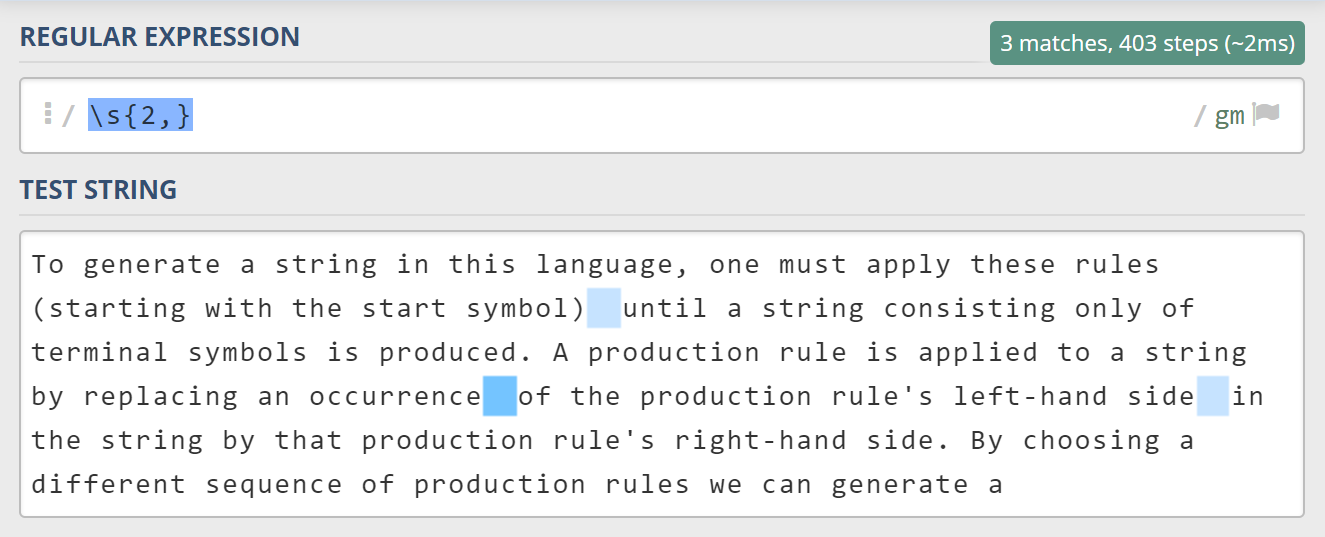
\includegraphics[width=\textwidth]{regex101_matching.png}}
  \caption{Screenshot of the Regex101's matching functionality. The user
  provided the ``\texttt{\textbackslash{}s\textbackslash{}s+}'' regular
  expression, which matched every occurrence of two or more consecutive space
  characters in the test string.}
  \label{fig:regex101-matching}
\end{figure}

The tool is available to users in the form of a web application and can be
accessed from \url{https://regex101.com/}. It lets users build expressions fast
and debug them along the way, for example by pasting in a set of data and then,
through trial and error, building an expression with desired behavior.
Figure~\ref{fig:regex101-matching} shows a typical usage of Regex101 ---
matching a pasted test string to a regular expression. The tool makes it clear
if data is matching the expression or not, it even notifies users when the
expression is broken, and gives some explanation of why it is not working, as
seen in figure~\ref{fig:regex101-error}.

\begin{figure}[ht]
  \centering
  \frame{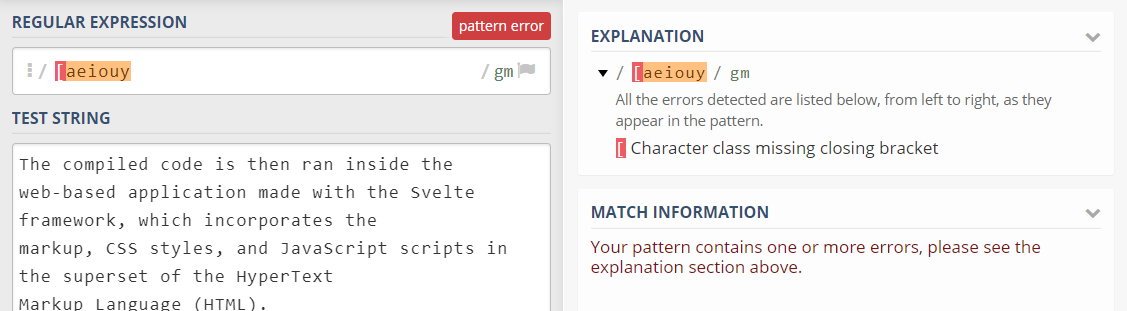
\includegraphics[width=\textwidth]{regex101_error.png}}
  \caption{Screenshot of a basic error in the regular expression reported by
  Regex101.}
  \label{fig:regex101-error}
\end{figure}

These two feedback mechanisms are really helpful if the user is not accustomed
with the regular expression language, or just does not know how to build the
right expression yet. Being able to trace each step of the expression is a true
lifesaver when users are not able to figure out why something is not working, or
even if they are simply interested in learning more about regular expressions.
Getting this instant feedback without Regex101 would have required users to
write their expressions in a text editor and then run the code separately,
without getting much feedback about why it is or isn't working. Regex101.com
eliminates this mystery.

Not only does Regex101.com make it easy to build expressions, find errors, and
even learn the syntax, it makes looking up a token or character in regular
expressions very easy. Always present, unless users minimize it, the \emph{Quick
Reference} tool lets them look up any token or character they need. Finally,
Regex101 lets users switch which \emph{flavor} or version of regular expressions
they wish to use, as they might need to integrate a regular expression
expression into any number of other programming languages such as Python,
JavaScript, Golang, etc. Regex101 has the ability to change the version of the
testing environment and will generate the code in that language for the user to
use in other projects.}

\thisproject{} takes a lot of inspiration from Regex101 when it comes to
availability --- it's a web application, where all the work is done client-side.
The user does not have to install any additional software except the web
browser, the web application is accessed through a web page. In spite of its
similar nature, Regex101 cannot be a replacement of \thisproject{} --- it
focuses on various dialects of regular expressions rather than parsing EBNF and
generating parse trees --- it does, however, influence it with its accessibility
and functionalities.

\section*{Pest}

Pest \cite{pest} is a general purpose parser for the Rust programming language.
It uses its own dialect of \emph{parsing expression grammars} as input,
similarly to \thisproject{}. Pest addresses the problem of hand-written parsers
in Rust, which in some circumstances can become hard to maintain by their
developers. Writing a specialized, domain-specific parser for a language can
become tedious, so developers usually gravitate towards using a
grammar-generated parser. This allows the developers to focus on the definition
of the language, rather than on the implementation of the parser.
\paraphrase{Grammars which define the language offer better correctness
guarantees, and issues can be solved declaratively in the grammar itself. Rust's
memory safety further limits the amount of damage bugs can do. High-level static
analysis and careful low-level implementation build a solid foundation on which
serious performance tuning is possible.}

Developers of Pest, in spite of focusing mainly on the functionalities in the
Rust programming language, also provide an online editor available from the
browser on the Pest's homepage (\url{https://pest.rs/#editor}). The online
editor allows potential future users of Pest to experience the syntactic
characteristics of the Pest's dialect of PEGs and its error reporting
capabilities. The editor will inform the user about any syntactic errors, as
well as errors of semantic nature, such as undefined or left-recursive
production rules (seen in figure~\ref{fig:pest-error}) and highlight them in
their exact locations.

\begin{figure}[ht]
  \centering
  \frame{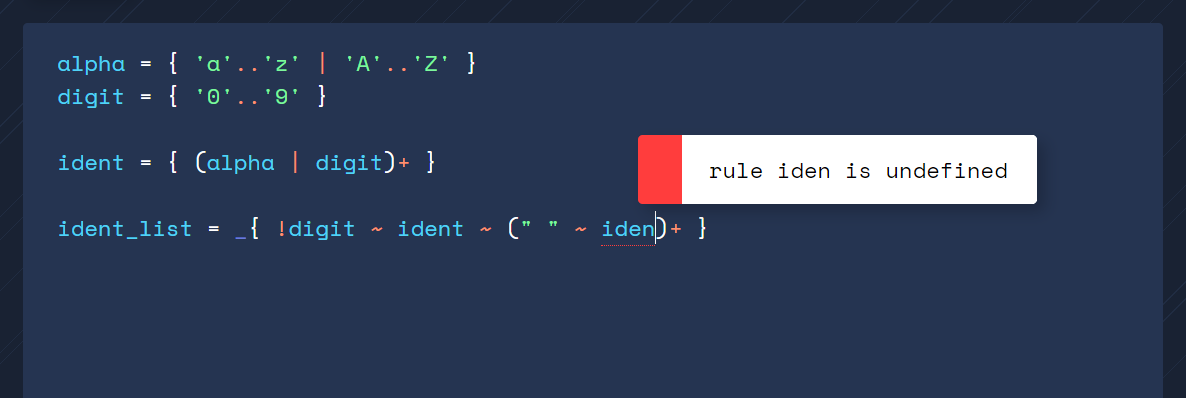
\includegraphics[width=\textwidth]{pest_error.png}}
  \caption{Screenshot of Pest's online editor example error report.}
  \label{fig:pest-error}
\end{figure}

After parsing the grammar, Pest provides a window, which acts as an input
console, where users can type string that may or may not be parsed by the parser
generated by Pest. Additionally, users can choose the initial production rule
from a dropdown menu, which is an interesting choice, as opposed to
automatically detecting the initial rule based on the dependency graph of
production rules. The output window presents the parse tree, or the errors
encountered in the input string in case there are any. These features can be
seen in figure~\ref{fig:pest-output}.

\begin{figure}[ht]
  \centering
  \frame{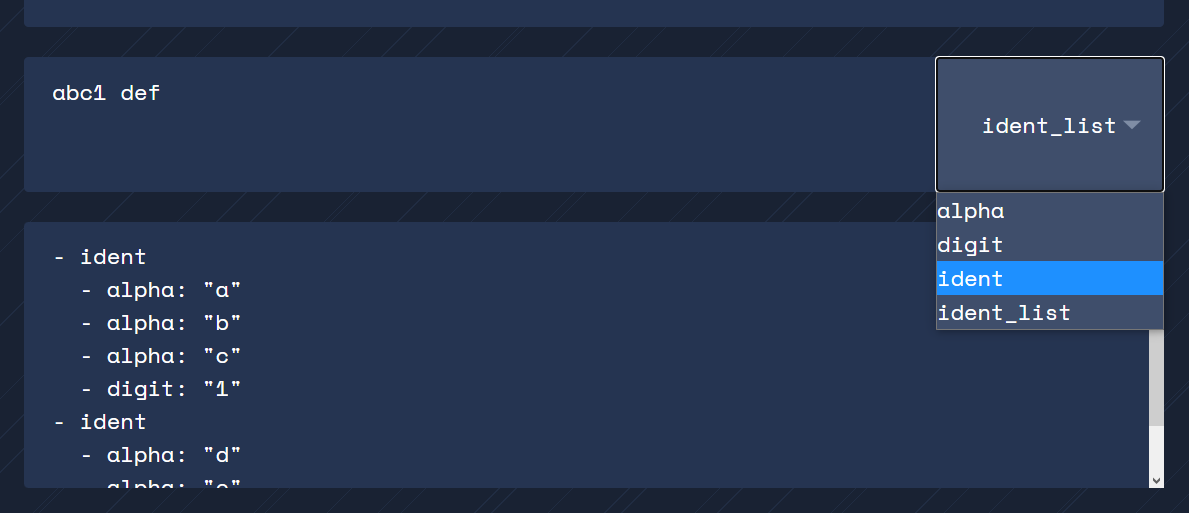
\includegraphics[width=\textwidth]{pest_output.png}}
  \caption{Screenshot of the input and output windows in Pest's online editor.}
  \label{fig:pest-output}
\end{figure}

While Pest focuses mainly on its integration with the Rust programming language,
this is not the case for \thisproject{}, which aims to provide all of its
functionality inside the web application. The online editor of Pest serves
largely as a ``try me'' feature for new users, rather than a reliable tool. The
editor lacks the standard editor features, such as autocompletion, code folding,
search and replace interface, as well as bracket and tag matching, all of which
\thisproject{} does provide. The parse tree in the output window is shown in a
basic textual form, without any interactive capabilities, which the user may
value. Finally, while Pest's grammar is based on PEGs, and is similar in nature
to EBNF, it is, in fact, not EBNF. The whole point of using EBNF and other
notations discussed in section~\ref{sec:why-ebnf} is that they're standardized,
well-known, and accepted by the community; Pest's syntax is known only to users
of Pest and requires them to learn a new, non-standard language just for the
purpose of parsing grammars, where other, already established languages may have
sufficed.

\chapter{Design of the project} \label{ch:design-of-the-project}

This chapter introduces a specification for the application described in
chapter~\ref{ch:problem-analysis}. The specification is presented in forms of a
list of functional and non-functional requirements in
section~\ref{sec:requirements}, and user stories in
section~\ref{sec:user-stories}. Section~\ref{sec:use-case-specification}
describes use cases and their descriptions structured in the form of a use case
diagram in the Unified Modeling Language, as well as their example scenarios,
also presented as activity and sequence diagrams. The chapter describes the
architecture of the system from the logical and physical perspective as
component and deployment diagrams in section~\ref{sec:system-architecture}. The
chapter does not cover any class or database diagrams, as the implementation of
this project and its functionally-oriented nature, as opposed to being
object-oriented, does not require them. Finally, the chapter concludes with the
prototype and sketches of the user interface for the web application in
section~\ref{sec:interface-prototype}.

\section{Requirements} \label{sec:requirements}

\subsection{Functional requirements}

Functional requirements shown in table~\ref{tab:functional-requirements} define
functionalities and features of the system. Each requirement is associated with
a certain priority.

\begin{xltabular}{\textwidth}{@{}lL{3cm}Xl@{}}
  \caption{The functional requirements of the project, their features, and
  priorities.}
  \label{tab:functional-requirements}\\
  \toprule
  Id & Requirement & Features & Priority \\* \midrule
  \endfirsthead
  %
  \endhead
  %
  \endfoot
  %
  \endlastfoot
  %
  \emph{FR1} & Specifying the grammar & The user can specify the grammar of a
  given language in the EBNF notation by providing it in a textual form in
  a designated editor window. & high \\
  \addlinespace[0.5em] \emph{FR2} & Error reporting & The editor provides
  feedback about any syntactic or semantic\footnote{Such as production
  rule duplication or left recursion.} errors encountered during the parsing by
  highlighting the exact location of the error in the provided grammar. The user
  can then hover the mouse pointer over the highlighted area to read the error
  message. & high \\
  \addlinespace[0.5em] \emph{FR3} & Specifying the input string & The user can
  specify the input string in a designated editor window to check if it
  belongs to the language generated by the previously-defined grammar. & high
  \\
  \addlinespace[0.5em] \emph{FR4} & Visualizing the parse tree & The
  application visualizes the parse tree resulting from parsing the specified
  input string with the parser generated by the grammar defined by the user. &
  high \\
  \addlinespace[0.5em] \emph{FR5} & Syntax highlighting & The editor highlights
  parts of the specified grammar with a different syntactic meaning in a
  different manner with the use of multi-colored fonts. & medium \\
  \addlinespace[0.5em] \emph{FR6} & Autocompletion of non-terminals & The
  editor predicts the identifier of a non-terminal a user is typing by
  providing a list of possible non-terminals, which then can be chosen by the
  user. & low \\
  \addlinespace[0.5em] \emph{FR7} & Production rule folding & The editor
  provides the ability to hide and reveal a production rule of the grammar
  inside the editor window. & low \\
  \addlinespace[0.5em] \emph{FR8} & Search and replace interface & The user can
  search for any occurrences of a phrase in the editor window and possibly
  replace them with a different phrase. The search and replace functionality
  should also support regular expressions. & low \\* \bottomrule
\end{xltabular}

\subsection{Non-functional requirements}

Table~\ref{tab:non-functional-requirements} describes requirements of the
non-functional nature of the system, which focus on aspects of usability,
availability, and compatibility of the system.

\begin{xltabular}{\textwidth}{@{}Xl@{}}
  \caption{The non-functional requirements of the project and their priorities.}
  \label{tab:non-functional-requirements}\\
  \toprule
  Requirement & Priority \\* \midrule
  \endfirsthead
  %
  \endhead
  %
  \endfoot
  %
  \endlastfoot
  %
  The web application should be available 24 hours a day, 7 days a week. &
  medium \\
  \addlinespace[0.5em] Page loading time should be less than 1 second with
  internet download speed of 80\,Mbps. Parsing and checking times should both
  be less than 50 milliseconds. & high \\
  \addlinespace[0.5em] The application must work and display correctly in
  \begin{itemize}[noitemsep,nolistsep]
    \item Chrome version 86 or later,
    \item Safari version 14 or later,
    \item Edge version 86 or later,
    \item Firefox version 82 or later,
    \item Opera version 71 or later. \end{itemize} & high \\
  & medium \\
  \addlinespace[0.5em] The source code of the product should be open source
  and freely available for possible modification and redistribution. & high \\
  \addlinespace[0.5em] The project should include the documentation necessary
  for extension and maintenance of the system. & high \\
  \addlinespace[0.5em] The system should provide high degree of integrability
  with future components which extend the functionalities of the system. & high
  \\* \bottomrule
\end{xltabular}

\section{User stories} \label{sec:user-stories}

Stories in table~\ref{tab:user-stories} are short descriptions of a feature told
from the perspective of the person who desires a new functionality in the
system.

\begin{xltabular}{\textwidth}{@{}lX@{}}
  \caption{The user stories.}
  \label{tab:user-stories}\\
  \toprule
  Id & User story \\* \midrule
  \endfirsthead
  %
  \endhead
  %
  \endfoot
  %
  \endlastfoot
  %
  \emph{US1} & As the user, I want to be able to paste the contents of my
  clipboard into the editor window in the application. \\
  \addlinespace[0.5em] \emph{US2} & As the user, I want to be able to type in
  the editor window with my keyboard. \\
  \addlinespace[0.5em] \emph{US3} & As the user, I want to be able to appreciate
  the multi-colored appearance of the text that represents the syntax that I
  provided. \\
  \addlinespace[0.5em] \emph{US4} & As the user, I want to be able to select a
  portion of the text in the editor window and copy it to the clipboard using a
  keyboard shortcut. \\
  \addlinespace[0.5em] \emph{US5} & As the user, I want to be able to hold the
  \emph{Alt} key on my keyboard to create multiple cursors in the editor window.
  \\
  \addlinespace[0.5em] \emph{US6} & As the user, I want to have the ability to
  autocomplete the non-terminal I am typing that has already been declared
  elsewhere in the code. \\
  \addlinespace[0.5em] \emph{US7} & As the user, I want to be able to hide any
  existing production rules that might appear too long, to increase the degree
  of clarity and readability of the grammar I'm working on. \\
  \addlinespace[0.5em] \emph{US8} & As the user, I want to be able to show any
  previously hidden production rules of the grammar. \\
  \addlinespace[0.5em] \emph{US9} & As the user, I want to have the ability to
  press a certain key combination on my keyboard that would allow me to type a
  specific phrase in the popup window, which would then find all the occurrences
  of that phrase in the editor window. \\
  \addlinespace[0.5em] \emph{US10} & As the user, I want to be able to provide a
  regular expression for the \emph{find} functionality that would allow me to
  find all occurrences of phrases that pattern match that specific regular
  expression. \\
  \addlinespace[0.5em] \emph{US11} & As the user, I want to be able to replace
  some of the occurrences of phrases found with the \emph{find} functionality
  with another phrase provided in a popup window. \\
  \addlinespace[0.5em] \emph{US12} & As the user, I want to be able to specify
  the initial production rule in the process of checking the input string
  against the grammar I provided. \\
  \addlinespace[0.5em] \emph{US13} & As the user, I want to be able to see
  errors in the syntax of the provided grammar in the form of underlined text in
  the location of where the errors actually occur. \\
  \addlinespace[0.5em] \emph{US14} & As the user, I want to have the ability to
  hover the mouse pointer over the underlined text to read the error message at
  that location. Alternatively, I want to be able to hover over the error
  indicator, which appears next to the line number. \\
  \addlinespace[0.5em] \emph{US15} & As the user, I want to be able to see the
  parse tree of the recognized input string that I provided. \\
  \addlinespace[0.5em] \emph{US16} & As the user, I want to have the ability to
  collapse any nodes in the visualized parse tree that might appear too long.
  \\* \bottomrule
\end{xltabular}

\section{Use case specification} \label{sec:use-case-specification}

\subsection{Use cases} \label{sbs:use-cases}

Figure~\ref{fig:use-case-diagram} shows the use case diagram of the system. Each
use case also presented in table~\ref{tab:use-cases} along with a short
description.

\begin{figure}[H]
  \centering
  \resizebox{0.75\textwidth}{!}{\fontsize{9}{10}\input{images/use_case_diagram.pdf_tex}}
  \caption{The use case diagram.}
  \label{fig:use-case-diagram}
\end{figure}

\begin{xltabular}{\textwidth}{@{}lL{3cm}Xl@{}}
  \caption{Descriptions of the use cases.}
  \label{tab:use-cases}\\
  \toprule
  Id & Name & Description \\* \midrule
  \endfirsthead
  %
  \endhead
  %
  \endfoot
  %
  \endlastfoot
  %
  \emph{UC1} & Specifying the grammar & Allows the user to specify the grammar
  of a given language in the EBNF notation by providing it in a textual form in
  a designated editor window. \\
  \addlinespace[0.5em] \emph{UC2} & Specifying the input string & Allows the
  user to specify the input string in a designated editor window to check if it
  belongs to the language generated by the previously-defined grammar. \\
  \addlinespace[0.5em] \emph{UC3} & Interacting with the visualization & Allows
  the user to observe the visualized parse tree of the provided input string and
  interact with it by expanding and collapsing the tree nodes. \\
  \addlinespace[0.5em] \emph{UC4} & Changing the initial rule & Allows the user
  to specify the initial production rule used in the process of checking the
  provided input string against the defined grammar. \\* \bottomrule
\end{xltabular}

\subsection{Requirements traceability graph}

Figure~\ref{fig:rtg} presents the relationship between functional requirements,
user stories and use cases in the form of a requirements traceability graph. It
shows that every user story is connected with at least one functional
requirement and vice versa, and that every use case is associated with at least
one user story and vice versa.

\begin{figure}[H]
  \centering
  \pgfdeclarelayer{bg}
  \pgfsetlayers{bg,main}
  \resizebox{\textwidth}{!}{%
    \begin{tikzpicture}[xscale=1.2,yscale=3]
      \tikzstyle{every node}=[draw,circle,minimum size=1cm,inner sep=0pt,fill=white]

      \node at (-1.5,-1) (uc1) {\emph{UC1}};
      \node at (-0.5,-1) (uc2) {\emph{UC2}};
      \node at (0.5,-1)  (uc3) {\emph{UC3}};
      \node at (1.5,-1)  (uc4) {\emph{UC3}};

      \node at (-7.5,0) (us1)  {\emph{US1}};
      \node at (-6.5,0) (us2)  {\emph{US2}};
      \node at (-5.5,0) (us3)  {\emph{US3}};
      \node at (-4.5,0) (us4)  {\emph{US4}};
      \node at (-3.5,0) (us5)  {\emph{US5}};
      \node at (-2.5,0) (us6)  {\emph{US6}};
      \node at (-1.5,0) (us7)  {\emph{US7}};
      \node at (-0.5,0) (us8)  {\emph{US8}};
      \node at (0.5,0) (us9)  {\emph{US9}};
      \node at (1.5,0) (us10) {\emph{US10}};
      \node at (2.5,0) (us11) {\emph{US11}};
      \node at (3.5,0) (us12) {\emph{US12}};
      \node at (4.5,0) (us13) {\emph{US13}};
      \node at (5.5,0) (us14) {\emph{US14}};
      \node at (6.5,0) (us15) {\emph{US15}};
      \node at (7.5,0) (us16) {\emph{US15}};

      \node at (-3.5,1) (fr1) {\emph{FR1}};
      \node at (-2.5,1) (fr2) {\emph{FR2}};
      \node at (-1.5,1) (fr3) {\emph{FR3}};
      \node at (-0.5,1) (fr4) {\emph{FR4}};
      \node at (0.5,1)  (fr5) {\emph{FR5}};
      \node at (1.5,1)  (fr6) {\emph{FR6}};
      \node at (2.5,1)  (fr7) {\emph{FR7}};
      \node at (3.5,1)  (fr8) {\emph{FR8}};

      \begin{pgfonlayer}{bg}
        \draw (fr1) -- (us1);
        \draw (fr1) -- (us2);
        \draw (fr1) -- (us4);
        \draw (fr1) -- (us5);
        \draw (fr2) -- (us13);
        \draw (fr2) -- (us14);
        \draw (fr3) -- (us1);
        \draw (fr3) -- (us2);
        \draw (fr3) -- (us4);
        \draw (fr3) -- (us5);
        \draw (fr4) -- (us15);
        \draw (fr4) -- (us16);
        \draw (fr5) -- (us3);
        \draw (fr6) -- (us6);
        \draw (fr7) -- (us7);
        \draw (fr7) -- (us8);
        \draw (fr8) -- (us9);
        \draw (fr8) -- (us10);
        \draw (fr8) -- (us11);

        \draw (us1) -- (uc1);
        \draw (us2) -- (uc1);
        \draw (us3) -- (uc1);
        \draw (us4) -- (uc1);
        \draw (us5) -- (uc1);
        \draw (us6) -- (uc1);
        \draw (us7) -- (uc1);
        \draw (us8) -- (uc1);
        \draw (us9) -- (uc1);
        \draw (us10) -- (uc1);
        \draw (us11) -- (uc1);
        \draw (us12) -- (uc1);
        \draw (us13) -- (uc1);
        \draw (us1) -- (uc2);
        \draw (us2) -- (uc2);
        \draw (us3) -- (uc2);
        \draw (us4) -- (uc2);
        \draw (us5) -- (uc2);
        \draw (us6) -- (uc2);
        \draw (us7) -- (uc2);
        \draw (us8) -- (uc2);
        \draw (us9) -- (uc2);
        \draw (us10) -- (uc2);
        \draw (us11) -- (uc2);
        \draw (us13) -- (uc2);
        \draw (us14) -- (uc2);
        \draw (us12) -- (uc3);
        \draw (us15) -- (uc4);
        \draw (us16) -- (uc4);
      \end{pgfonlayer}
    \end{tikzpicture}
  }
  \caption{The requirements traceability graph.}
  \label{fig:rtg}
\end{figure}

\subsection{Use case scenarios} \label{sbs:use-case-scenarios}

Tables~\ref{tab:uc1-scenario}, \ref{tab:uc2-scenario}, \ref{tab:uc3-scenario},
and \ref{tab:uc4-scenario} describe the scenarios of each use case in the
system. Every scenario is defined by its pre-conditions, its post-conditions,
and a list of steps made by the system or the user required to complete it.

\begin{xltabular}{\textwidth}{@{}L{3cm}X@{}}
  \caption{Use case scenario of \emph{UC1} Specifying the grammar.}
  \label{tab:uc1-scenario}\\
  \toprule
  \endfirsthead
  %
  \endhead
  %
  \endfoot
  %
  \endlastfoot
  %
  Identifier & \emph{UC1} \\
  \addlinespace[0.5em] Name & Specifying the grammar \\
  \addlinespace[0.5em] Summary & Allows the user to specify the grammar of a
  given language in the EBNF notation by providing it in a textual form in a
  designated editor window. \\
  \addlinespace[0.5em] Pre-conditions & None. \\
  \addlinespace[0.5em] Post-conditions & The grammar has been correctly defined
  by the user with no syntactic errors. \\
  \addlinespace[0.5em] Main scenario &
  \begin{enumerate}[noitemsep,nolistsep,labelindent=0.5cm,align=right]
    \item [1.] The system shows a grammar editor window to the user.
    \item [2.] The user provides a syntactically and semantically correct
    definition of a grammar.
    \item [3.] The system shows an icon indicating no errors detected in the
    grammar.
    \item [] End of scenario.
  \end{enumerate} \\
  \addlinespace[0.5em] Alternative scenario &
  \begin{enumerate}[noitemsep,nolistsep,labelindent=0.5cm,align=right]
    \item [2a.1.] The user provides an invalid definition of a grammar.
    \item [2a.2.] The system highlights the text in the grammar editor window at
    the error location.
    \item [] Return to step 2.
  \end{enumerate} \\* \bottomrule
\end{xltabular}

\begin{xltabular}{\textwidth}{@{}L{3cm}X@{}}
  \caption{Use case scenario of \emph{UC2} Specifying the input string.}
  \label{tab:uc2-scenario}\\
  \toprule
  \endfirsthead
  %
  \endhead
  %
  \endfoot
  %
  \endlastfoot
  %
  Identifier & \emph{UC2} \\
  \addlinespace[0.5em] Name & Specifying the input string \\
  \addlinespace[0.5em] Summary & Allows the user to specify the input string in
  a designated editor window to check if it belongs to the language generated by
  the previously-defined grammar. \\
  \addlinespace[0.5em] Pre-conditions & None. \\
  \addlinespace[0.5em] Post-conditions & The input string has been correctly
  entered by the user. \\
  \addlinespace[0.5em] Main scenario &
  \begin{enumerate}[noitemsep,nolistsep,labelindent=0.5cm,align=right]
    \item [1.] The system shows a input string editor window to the user.
    \item [2.] The user provides a desired input string.
    \item [3.] A valid grammar has been provided by the user in the grammar
    editor window.
    \item [4.] The system shows the result of the checker in the result window.
    \item [] End of scenario.
  \end{enumerate} \\
  \addlinespace[0.5em] Alternative scenario &
  \begin{enumerate}[noitemsep,nolistsep,labelindent=0.5cm,align=right]
    \item [3a.1.] The user did not provide a valid grammar in the grammar editor
    window.
    \item [3a.2.] The system does not show a result of the checker.
    \item [] End of scenario.
  \end{enumerate} \\* \bottomrule
\end{xltabular}

\begin{xltabular}{\textwidth}{@{}L{3cm}X@{}}
  \caption{Use case scenario of \emph{UC3} Interacting with the visualization.}
  \label{tab:uc3-scenario}\\
  \toprule
  \endfirsthead
  %
  \endhead
  %
  \endfoot
  %
  \endlastfoot
  %
  Identifier & \emph{UC3} \\
  \addlinespace[0.5em] Name & Interacting with the visualization \\
  \addlinespace[0.5em] Summary & Allows the user to observe the visualized parse
  tree of the provided input string and interact with it by expanding and
  collapsing the tree nodes. \\
  \addlinespace[0.5em] Pre-conditions & The user has provided a valid definition
  of a grammar, as well as an input string, that belongs to the language
  generated by that grammar. \\
  \addlinespace[0.5em] Post-conditions & None. \\
  \addlinespace[0.5em] Main scenario &
  \begin{enumerate}[noitemsep,nolistsep,labelindent=0.5cm,align=right]
    \item [1.] The system shows the result of a checker in the form of a
    visualized parse tree.
    \item [2.] The user clicks the nodes of the parse tree to collapse or
    expand them.
    \item [] End of scenario.
  \end{enumerate} \\* \bottomrule
\end{xltabular}

\begin{xltabular}{\textwidth}{@{}L{3cm}X@{}}
  \caption{Use case scenario of \emph{UC2} Specifying the input string.}
  \label{tab:uc4-scenario}\\
  \toprule
  \endfirsthead
  %
  \endhead
  %
  \endfoot
  %
  \endlastfoot
  %
  Identifier & \emph{UC4} \\
  \addlinespace[0.5em] Name & Changing the initial rule \\
  \addlinespace[0.5em] Summary & Allows the user to specify the initial
  production rule used in the process of checking the provided input string
  against the defined grammar. \\
  \addlinespace[0.5em] Pre-conditions & The user has provided a valid definition
  of a grammar. \\
  \addlinespace[0.5em] Post-conditions & The initial production rule has been
  successfully changed to the desired one. \\
  \addlinespace[0.5em] Main scenario &
  \begin{enumerate}[noitemsep,nolistsep,labelindent=0.5cm,align=right]
    \item [1.] The system shows a button the current initial production rule
    written on top.
    \item [2.] The user clicks on the button.
    \item [3.] The system shows a dropdown menu with a list of all production
    rules defined in the provided grammar.
    \item [4.] The user clicks on an item of the list corresponding to the
    desired initial production rule.
    \item [5.] The system changes the identifier of the initial production rule
    on the button.
    \item [] End of scenario.
  \end{enumerate} \\* \bottomrule
\end{xltabular}

\subsection{Activity diagrams}

Figures~\ref{fig:uc1-activity-diagram}, \ref{fig:uc2-activity-diagram},
\ref{fig:uc3-activity-diagram}, and \ref{fig:uc4-activity-diagram} are the
graphical representations of use case scenarios defined in subsection
\ref{sbs:use-case-scenarios}, represented in the form of UML activity diagrams.

\begin{figure}[H]
  \centering
  \resizebox{!}{5cm}{\footnotesize\input{images/uc1_activity_diagram.pdf_tex}}
  \caption{The activity diagram of \emph{UC1} Specifying the grammar.}
  \label{fig:uc1-activity-diagram}
\end{figure}

\begin{figure}[H]
  \centering
  \resizebox{!}{5cm}{\footnotesize\input{images/uc2_activity_diagram.pdf_tex}}
  \caption{The activity diagram of \emph{UC2} Specifying the input string.}
  \label{fig:uc2-activity-diagram}
\end{figure}

\begin{figure}[H]
  \centering
  \resizebox{!}{5cm}{\footnotesize\input{images/uc3_activity_diagram.pdf_tex}}
  \caption{The activity diagram of \emph{UC3} Interacting with the
  \label{fig:uc3-activity-diagram}
  visualization.}
\end{figure}

\begin{figure}[H]
  \centering
  \resizebox{!}{5cm}{\footnotesize\input{images/uc4_activity_diagram.pdf_tex}}
  \caption{The activity diagram of \emph{UC4} Changing the initial rule.}
  \label{fig:uc4-activity-diagram}
\end{figure}

\subsection{Sequence diagram}

Figure~\ref{fig:sequence-diagram} shows a sequence diagram, that is in essence
an interaction diagram that details how operations in the system are carried out
and visualizes interactions between objects and components. It captures
interactions from every use case, all of which were defined in
subsection~\ref{sbs:use-cases}.

\begin{figure}[H]
  \centering
  \resizebox{0.65\textwidth}{!}{\footnotesize\input{images/sequence_diagram_1.pdf_tex}}
  \caption{The sequence diagram representing the specification of the grammar.}
  \label{fig:sequence-diagram}
\end{figure}

\newpage

\section{System architecture} \label{sec:system-architecture}

\subsection{Logical architecture}

Logical architecture of a system can be represented by UML component diagrams,
which focus on a system's components that are often used to model the static
implementation view of a system. \paraphrase{A component diagram breaks down the
system into various high levels of functionality. Each component is responsible
for one clear aim within the entire system and only interacts with other
essential elements on a need-to-know basis.} In a system with a
functional-oriented approach it is more suitable for modelling interactions
between components. The logical architecture of \thisproject{} is modelled with
such a diagram and can be seen in figure~\ref{fig:logical-architecture}.

\begin{figure}[H]
  \centering
  \resizebox{0.8\textwidth}{!}{\small\input{images/logical_architecture.pdf_tex}}
  \caption{The logical architecture of the system represented with a UML
  component diagram.}
  \label{fig:logical-architecture}
\end{figure}

\subsection{Physical architecture}

A deployment diagram in the Unified Modeling Language models the physical
deployment of artifacts on nodes and can represent a physical architecture of
a system. Diagram shown on figure~\ref{fig:physical-architecture} visualizes
the architecture for \thisproject{}.

\begin{figure}[H]
  \centering
  \resizebox{\textwidth}{!}{\footnotesize\input{images/physical_architecture.pdf_tex}}
  \caption{The physical architecture of the system represented with a UML
  deployment diagram.}
  \label{fig:physical-architecture}
\end{figure}

\section{Interface prototype} \label{sec:interface-prototype}

Because of the visual nature of the web application, a prototype of the user
interface design should be established to allow the developer to plan out the
implementation of the front-end aspect of the application. \thisproject{}, being
a rather simple application, will consist of a single view (as seen in
figure~\ref{fig:interface-prototype}), which is made out of several components.

\begin{figure}[H]
  \centering
  \begin{tikzpicture}
    \draw (0,0) rectangle (12,9) node[pos=.5] {\todo{}};
  \end{tikzpicture}
  \caption{The user interface sketch.}
  \label{fig:interface-prototype}
\end{figure}

\chapter{Implementation of the project} \label{ch:implementation-of-the-project}

\section{Software environment}

\subsection{Used technologies} \label{sbs:used-technologies}

\subsubsection*{Visual Studio Code}

Visual Studio Code \cite{vs-code} is a free, open-source text editor made by
Microsoft for Windows, Linux and macOS. It is designed to write code and
features syntax highlighting, code completion, snippets, code refactoring, and
code debugging. The editor can be used with various programming languages, and
supports extensions, which can be installed through a central repository called
VS Code Marketplace available in the editor itself. The extensions may provide
feature additions to the editor, as well as the support for various programming
languages in the form of code linters, static code analysers, and debuggers. The
editor is integrated with various version control systems, including Git and
Subversion

According to the 2019 Developers Survey of Stack Overflow, Visual Studio Code
ranked \#1 among the top popular developer tools, with $50.7\,\%$ of the 87317
respondents using it. \cite{stack-overflow-insights-2019}

The extensions for the editor are created by the members of Visual Studio Code
community. Two main extensions used by the author to develop the project were:
\begin{description}
  \item[rust-analyzer] \cite{rust-analyzer} An implementation of the Language
  Server Protocol for the Rust programming language, which provides features
  such as code completion, messages for syntax and semantic errors, code
  actions, diagnostics, ``go to definition'' and other editor actions.
  \item[Svelte for VS Code] \cite{svelte-for-vs-code} An implementation of the
  Language Server Protocol for the Svelte framework. The extension provides
  diagnostic messages for warnings and errors, support for Svelte pre-processors
  that provide source maps, as well as the support for Svelte-specific
  formatting (via prettier-plugin-svelte). Besides the Svelte language, the
  extension supports features such as hover info, messages for syntax and lint
  errors, and autocompletions for HTML, CSS/SCSS/LESS, as well as TypeScript and
  JavaScript.
\end{description}
The extensions have not proven to be crucial for the development of the project,
but were an excellent addition to the workflow.

Besides the editor extensions, the terminal integrated with Visual Studio Code
editor has been a valuable feature throughout the development process. The
command line is a substantial factor in the development of modern applications,
so a built-in terminal window allows the user to swiftly switch between the code
editor and the command line.

The support for the Git version control system has also been advantageous when
it comes to code editing. Every added, modified, or removed line of code is
highlighted with an appropriate color in the code editor. This greatly improves
the readability of the code, and allows the users to revert the code to its
previous state right from the editor without any external tools.

\subsubsection*{Git}

Git \cite{git} is a free and open source distributed version control system. It
has been a major part of the development process for the project, and has been
used mainly as a tool for keeping track of the changes made to the source code
and for integrating features in a smooth, non-disruptive manner.

Git supports branching and merging, which means that several project features
may be implemented simultaneously and independently on separate \emph{branches}
and then \emph{merged} into the main project. Every major code change has been
implemented on a designated branch and was merged into the main branch only
after a thorough testing process --- this has made parallel development very
easy, by isolating new development from finished work. This style of a workflow
is known as GitFlow, made popular by Vincent Driessen \cite{git-flow}, it has
shown itself to be very effective for projects of any scale. Efficient switching
between different versions of project files enables developers to work
effectively on the project. Git includes specific tools for visualizing and
navigating a non-linear development history. The author used \cite{chacon-2014}
as a reference for using the tool.

Git is now the most widely used source-code management tool, with $87.2\,\%$ of
the 74298 respondents of the 2018 Developers Survey of Stack Overflow reporting
that they use Git as their primary source-control system.
\cite{stack-overflow-insights-2018}.

The main client of Git used in the project was the command-line tool on the
Ubuntu operating system running on Windows Subsystem for Linux.
Figure~\ref{fig:git} shows an example of GitFlow's \emph{feature branches} and
changes in the project repository in the Git version control system.

\begin{figure}[h]
  \centering
  \frame{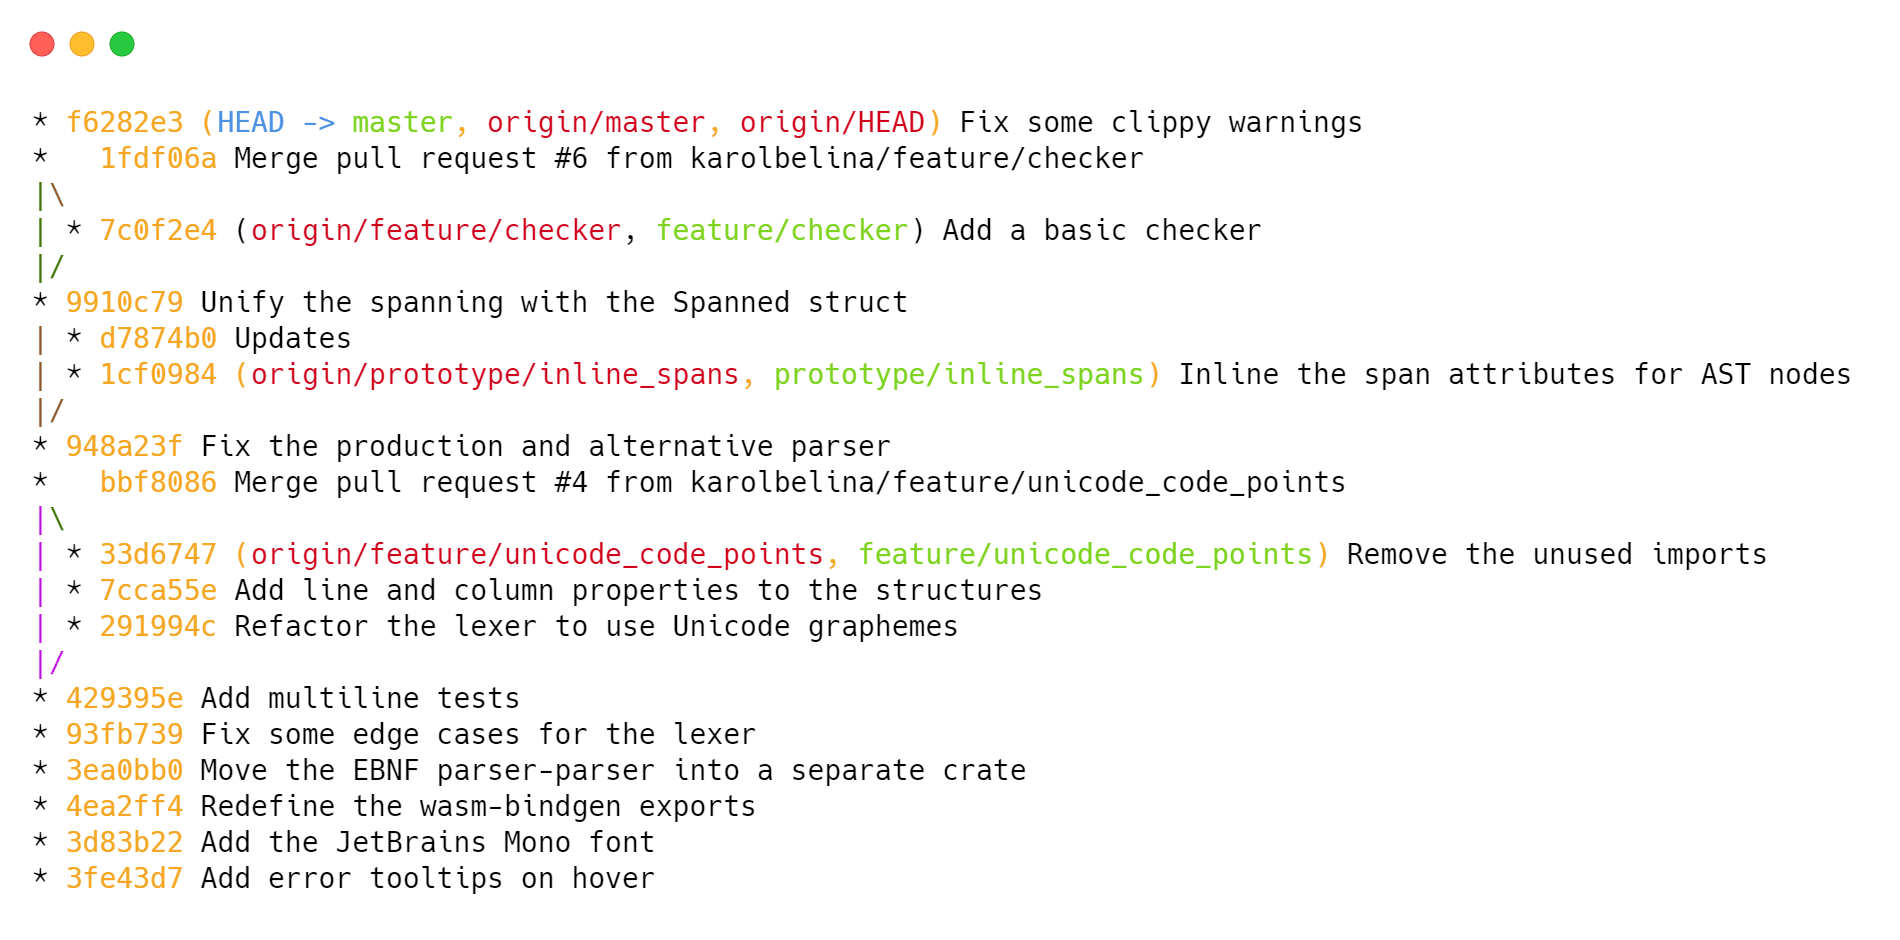
\includegraphics[width=\textwidth]{git.png}}
  \caption{Screenshot of the command-line interface of the Git version control
  system.}
  \label{fig:git}
\end{figure}

\subsubsection*{GitHub}

GitHub \cite{github} is a for-profit company owned by Microsoft that offers a cloud-based Git
repository hosting service. As a company, GitHub makes money by selling hosted
private code repositories, as well as other business-focused plans that make it
easier for organizations to manage team members and security. The author used
the free GitHub plan as the service for hosting the project's Git repository.
Having the source code on an external server protected the project against data
loss and allowed the developer to work on the project from any device at any
convenient time.

In addition to using GitHub as a hosting service, one can also exploit its
project management features. Developers can create project boards related to the
project's code repository, which are simple kanban board that can help organize
and prioritize the work. With projects, the developers have the flexibility to
manage boards for an entire project, or just for specific features.
Figure~\ref{fig:github-projects} shows an example project board from
\thisproject{}.

Project boards contain \emph{issues} and \emph{pull requests}, which can be
moved from one kanban column to another, indicating that some work is currently
``to do'', work in progress, or complete. These work ``cards'' contain
information about the author, assignees, the status, as well as simple textual
notes. The \emph{issues} are a way of reporting ideas, bugs, enhancements, or
tasks natively on GitHub. After completing the work on an issue, a developer
might create a \emph{pull request} to allow other developers on the project to
review and discuss the changes made to the code, and then deploy the changes by
``pulling'' the code to the central code repository.

\begin{figure}[h]
  \centering
  \frame{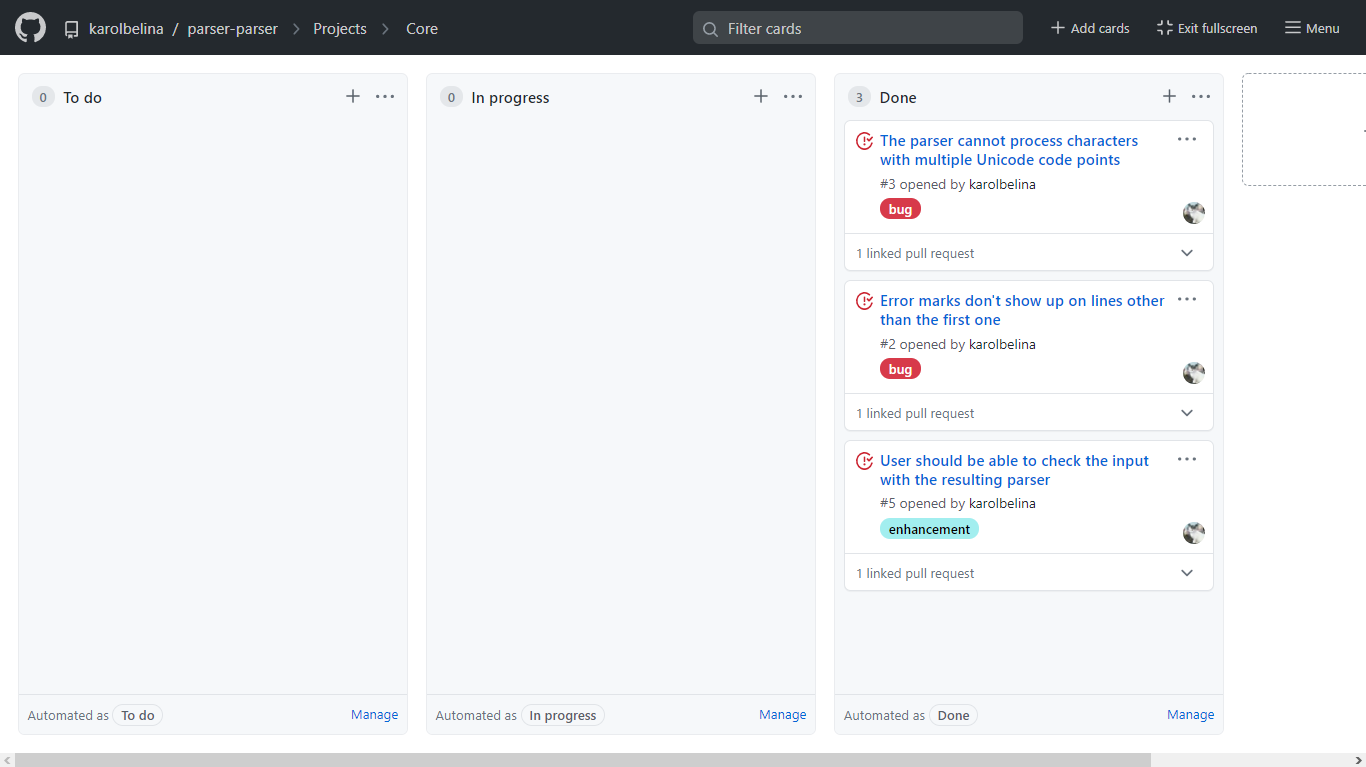
\includegraphics[width=\textwidth]{github_projects.png}}
  \caption{Screenshot of one of the project's kanban boards on GitHub.}
  \label{fig:github-projects}
\end{figure}

GitHub supports Continuous integration and Continuous Delivery functionalities
in form of \emph{Actions} and \emph{Pages}. GitHub Actions are a way to automate
and execute any software development workflow after any change to the code in
the repository. The user may set up many various actions for testing the changes
on many development environments and operating systems at the same time, as well
as building and deploying the code as a package or an arbitrary artifact. An
action consists of jobs, which are defined by a list of steps required to
execute them.

The GitHub Actions are used by the author to automate the testing and build
process on every change made to the code repository. The built application is
then deployed to a static site hosting service called GitHub Pages, which
integrates itself seamlessly with Actions and GitHub repositories. GitHub Pages
allows the user to host a website directly from a GitHub repository by combining
static HTML, CSS, JavaScript, and other files straight from a repository into
a website and publishing it on a \texttt{github.io} domain or a custom one.

\subsubsection*{Rust}

Rust \cite{rust} is the main programming language used in \thisproject{} --- it
powers the business logic part of the project. The language has been the most
loved language for four years in a row in the Stack Overflow's survey
\cite{stack-overflow-insights-2019}. The core idea of the language is memory
safety --- the language enforces certain rules checked at compile time, which
guarantee that the program is safe from bugs like dereferencing null or dangling
pointers, as well as making it difficult for the programmer to leak memory. Rust
does this through a system of ownership and borrowing. The language, besides the
safety, focuses on speed --- its design lets the developer create programs that
have the performance and control of a low-level language, but with the powerful
abstractions of a high-level language.

Rust's design borrows heavily from the one of Haskell --- both languages feature
a rich type system, both are immutable-by-default, avoid mutation of shared
references et cetera. Many developers tend to write Rust code in a functional
style and adhere to the principles of functional programming, even though the
language is multi-paradigm.

Without the need of a garbage collector, Rust projects are well-suited to be
used as libraries by other programming languages. The language over the last few
years has manifested itself in several distinct domains, including command-line
tools, networking, and embedded systems. Rust is supported on multiple operating
systems and targets multiple platforms, has notable documentation, a
user-friendly compiler with convenient error messages, and excellent tooling and
ecosystem. For referencing the language, the author used \cite{klabnik-2018},
which covers many features and concepts of Rust.

\subsubsection*{WebAssembly}

WebAssembly \cite{webassembly} (abbreviated \emph{Wasm}) is a safe, portable,
low-level code format designed for efficient execution and compact
representation. Its main goal is to enable high performance applications on the
Web, working alongside JavaScript, but not to be a replacement of it.
\paraphrase{It is designed to be portable, compact, and execute at or near
native speeds. Although it has currently gathered attention in the JavaScript
and Web communities in general, Wasm makes no assumptions about its host
environment.} WebAssembly is supported as a target for many programming
languages, including C$\sharp$ via Blazor, C++ via EmScripten, and the main
language used in \thisproject{} --- Rust. The author compiles Rust code to
WebAssembly to be then used in a web environment for several reasons:
\begin{itemize}
  \item \paraphrase{Code size is incredibly important since the \texttt{.wasm}
  file must be downloaded over the network. Rust lacks a runtime, enabling small
  Wasm sizes because there is no extra code included, like a garbage collector},
  \item \paraphrase{Rust and WebAssembly integrates with existing JavaScript
  tooling. It supports ECMAScript modules and the developer can continue using
  the tooling their already use, like npm and Webpack},
  \item \paraphrase{JavaScript Web applications struggle to attain and retain
  reliable performance.} The code is required to be ran frequently, so Wasm can
  solve this kind of problem \paraphrase{with better memory and CPU efficiency
  at a lower level compared to the JavaScript interpreter}.
  \item The Rust language itself, with a strong package manager, high
  performance, memory safety, and zero-cost abstractions.
\end{itemize}

\subsubsection*{Cargo}

Cargo is the Rust's package manager. \paraphrase{It downloads the Rust package's
dependencies and compiles them, ensuring that the developer will always get a
repeatable build. To accomplish this goal, Cargo introduces two metadata files
with various bits of package information, fetches and builds the dependencies,
invokes the Rust compiler with correct parameters to build the package, and
introduces conventions to make working with Rust packages easier.}

Rust provides first-class support for unit and integration testing, and Cargo
allows the developer to execute all tests with a single command. Additionally,
Cargo allows the developer to install extensions, which enhance the workflow and
the development process. One of extensions useful for the author was Clippy ---
a collection of lints to catch common mistakes and improve the Rust code.

\texttt{crates.io} \paraphrase{is the Rust community's central package registry
that serves as a location to discover and download packages. Cargo is configured
to use it by default to find requested packages.} The project uses several
dependencies, the most important of which include:
\begin{description}
  \item[nom] \cite{nom,couprie-2015} \paraphrase{A parser combinators library for Rust. Its
  goal is to provide tools to build safe parsers without compromising the speed
  or memory consumption. To that end, it uses extensively Rust's strong typing
  and memory safety to produce fast and correct parsers, and provides functions,
  macros and traits to abstract most of the error prone details.

  While programming language parsers are usually written manually for more
  flexibility and performance, nom can be (and has been successfully) used as a
  prototyping parser for a language. The resulting code is small, and looks like
  the grammar the developer would have written with other parser approaches. The
  resulting parsers are small and easy to write, as well as easy to test
  separately.}
  \item[unicode-segmentation] \cite{unicode-segmentation} A library with a set
  of iterators which split strings on \emph{grapheme clusters}, \emph{words} or
  \emph{sentence boundaries}, according to the Unicode Standard Annex \#29
  \cite{unicode-standard-annex-29} rules.
  \item[wasm-bindgen] \cite{wasm-bindgen} \paraphrase{A Rust library and CLI
  tool that facilitate high-level interactions between Wasm modules and
  JavaScript. More specifically, this library allows JavaScript and Wasm to
  communicate with strings, JS objects, classes, etc, as opposed to purely
  integers and floats. Notable features of this project include:
  \begin{itemize}
    \item Importing JS functionality into Rust such as DOM manipulation, console
    logging, or performance monitoring.
    \item Working with rich types like strings, numbers, classes, closures, and
    objects.
    \item Automatically generating TypeScript bindings for Rust code being
    consumed by JS.
  \end{itemize}
  Wasm-bindgen only generates bindings and glue for the JavaScript imports that
  are actually being used and Rust functionality that is being exported.}
  \item[quickcheck] A property-based testing framework inspired by the
  QuickCheck framework for Haskell. The crate comes with the ability to randomly
  generate and shrink integers, floats, tuples, booleans, lists, strings,
  options and results. All QuickCheck needs is a property function --- it will
  then randomly generate inputs to that function and call the property for each
  set of inputs. If the property fails (whether by a runtime error like index
  out-of-bounds or by not satisfying the property), the inputs are "shrunk" to
  find a smaller counter-example.
  \item[criterion] Provides a powerful but simple way to measure software
  performance. It provides both a framework for executing and analyzing
  benchmarks and a set of driver functions that makes it easy to build and run
  benchmarks, and to analyse their results.
  \item[structopt] Parses command-line arguments by defining a struct. StructOpt
  combines the Clap library with a custom derive for marking a struct containing
  values that will be translated into specific command-line arguments based on
  their types and markers. Besides the desired arguments, StructOpt
  automatically generates the \emph{help} string, which can be invoked with the
  \texttt{--help} flag, as well as a \texttt{--version} flag for checking the
  version of the program.
\end{description}
All of the above dependencies are available under the MIT license.

\subsubsection*{Wasm-pack}

Wasm-pack is a tool for building and working with Rust-generated WebAssembly
that the developer would like to interop with JavaScript, in the browser, or
with Node.js. The generated WebAssembly packages then could be published to the
npm registry, or otherwise used alongside any JavaScript packages in workflows
that the developer already uses, such as Webpack or Rollup. The tool
interoperates and utilizes the wasm-bindgen, another tool, to provide a bridge
between the types of JavaScript and Rust. It allows JavaScript to call a Rust
API with a string, or a Rust function to catch a JavaScript exception. wasm-pack
wraps the CLI portion of the wasm-bindgen tool. This results in wrapping the
WebAssembly module in JS wrappers which make it easier to interact with the
module. Wasm-bindgen supports both ES6 modules and CommonJS and the developer
can use wasm-pack to produce either type of package.

\subsubsection*{Svelte}

Svelte \cite{svelte} is a free and open-source front end JavaScript framework.
Svelte has its own compiler for converting app code into client-side JavaScript
at build time. \paraphrase{The developer writes the components using HTML, CSS
and JavaScript and during the build process Svelte compiles them into small
standalone JavaScript modules. While frameworks like React and Vue do the bulk
of their work in the user's browser while the app is running, Svelte shifts that
work into a compile step that happens only when the developer builds their app,
producing highly-optimized vanilla JavaScript. By statically analysing the
component template, the compiler can make sure that the browser does as little
work as possible. The outcome of this approach is not only smaller application
bundles and better performance, but also a developer experience that is more
approachable for people that have limited experience of the modern tooling
ecosystem. Svelte is particularly appropriate to tackle the following
situations:
\begin{itemize}
  \item Web applications intended for low power devices: Applications built with
  Svelte have smaller bundle sizes, which is ideal for devices with slow network
  connections and limited processing power.
  \item Highly interactive pages or complex visualizations: If the user is
  building data-visualizations that need to display a large number of DOM
  elements, the performance gains that come from a framework with no runtime
  overhead will ensure that user interactions are responsive.
  \item Onboarding people with basic web development knowledge: Svelte has a
  shallow learning curve. Web developers with basic HTML, CSS, and JavaScript
  knowledge can easily grasp Svelte specifics in a short time and start building
  web applications.
\end{itemize}

Being a compiler, Svelte can extend HTML, CSS, and JavaScript, generating
optimal JavaScript code without any runtime overhead. To achieve this, Svelte
extends vanilla web technologies and only intervenes in very specific situations
and only in the context of Svelte components.}

\subsubsection*{Rollup}

\paraphrase{Rollup \cite{rollup} is a module bundler for JavaScript which
compiles small pieces of code into a complex library or application. It uses the
standardized ES module format for code, which lets the developer freely and
seamlessly combine individual functions and external libraries. Rollup can
optimize ES modules for faster native loading in modern browsers, or output a
legacy module format.

By dividing the project into smaller separate pieces, the development process is
often times more straightforward, since that usually removes unexpected
interactions and dramatically reduces the complexity of the problems the
developer needs to solve, and simply writing smaller projects in the first place
isn't necessarily the answer. Unfortunately, JavaScript has not historically
included this capability as a core feature in the language. This finally changed
with the ES6 revision of JavaScript, which includes a syntax for importing and
exporting functions and data so they can be shared between separate scripts. The
specification is now fixed, but it is only implemented in modern browsers.
Rollup allows the user to write code using the new module system, and will then
compile it back down to existing supported formats such as CommonJS modules, AMD
modules, and IIFE-style scripts. This means that the developer gets to write
future-proof code.

In addition to enabling the use of ES modules, Rollup also statically analyzes
the imported code, and will exclude anything that isn't actually used. This
allows the user to build on top of existing tools and modules without adding
extra dependencies or bloating the size of the project. Because Rollup includes
the bare minimum, it results in lighter, faster, and less complicated libraries
and applications. Since this approach can utilise explicit \texttt{import} and
\texttt{export} statements, it is more effective than simply running an
automated \emph{minifier} to detect unused variables in the compiled output
code.}

\subsubsection*{npm}

\paraphrase{Node Package Manager is a package manager for the JavaScript
programming language. It consists of a command-line client, also called npm, and
an online database of public and paid-for private packages, called the npm
registry. The registry is accessed via the client, and the available packages
can be browsed and searched via the npm website.}

Npm provides several built-in scripts and allows users to define their own.
\paraphrase{An npm script is a convenient way to bundle common shell commands
for the project. They are typically commands, or a string of commands, which
would normally be entered at the command line in order to do something with the
application. Scripts are stored in a project's configuration file, which means
they're shared amongst everyone using the codebase. They help automate
repetitive tasks, and mean having to learn fewer tools. Scripts also ensure that
everyone is using the same command with the same flags. Common use cases for npm
scripts include building the project, starting a development server, compiling
CSS, linting, or minifying.}

The project is dependent on several npm packages:
\begin{description}
  \item[CodeMirror] \cite{codemirror} \paraphrase{A versatile text editor
  implemented in JavaScript for the browser. It is specialized for editing code,
  and comes with a number of language modes and addons that implement more
  advanced editing functionality. A rich programming API and a CSS theming
  system are available for customizing CodeMirror to fit the needs, as well as
  extending it with new functionality. It is the editor used in the dev tools
  for Firefox, Chrome, and Safari, in Light Table, Adobe Brackets, Bitbucket,
  and many other projects.}

  CodeMirror supports a wide variety of configurations --- the basic version of
  the editor without any addons provides the support for over 100 languages,
  autocompletion, code folding, configurable keybindings, search and replace
  interface, bracket and tag matching, support for split view, linter
  integration, various themes, and many more.
  \item[svelte-tree] A tree-like view component for Svelte. The component has
  the ability to display a collapsable tree structure based on a provided tree
  of JavaScript objects with custom \texttt{name} and \texttt{children}
  properties. The component provides a slot space to display custom nodes, which
  will give the tree node DOM/components the access to the nodes being rendered.
\end{description}
The configuration file also lists dependencies for the development process,
which can be divided into several categories:
\begin{itemize}
  \item Rollup and its plugins
  \begin{itemize}[noitemsep,nolistsep]
    \item \texttt{rollup},
    \item \texttt{@rollup/plugin-alias},
    \item \texttt{@rollup/plugin-commonjs},
    \item \texttt{@rollup/plugin-node-resolve},
    \item \texttt{@rollup/plugin-typescript},
    \item \texttt{@wasm-tool/rollup-plugin-rust},
    \item \texttt{rollup-plugin-copy},
    \item \texttt{rollup-plugin-css-only},
    \item \texttt{rollup-plugin-livereload},
    \item \texttt{rollup-plugin-svelte},
    \item \texttt{rollup-plugin-terser}
  \end{itemize}
  \item Svelte and its plugins
  \begin{itemize}[noitemsep,nolistsep]
    \item \texttt{svelte},
    \item \texttt{svelte-check},
    \item \texttt{svelte-loader},
    \item \texttt{svelte-preprocess}
  \end{itemize}
  \item Miscellaneous dependencies
  \begin{itemize}[noitemsep,nolistsep]
    \item \texttt{gh-pages},
    \item \texttt{prettier},
    \item \texttt{prettier-plugin-svelte},
    \item \texttt{rimraf},
    \item \texttt{sirv-cli}
  \end{itemize}
\end{itemize}

\newpage

\subsection{Project structure} \label{sbs:project-structure}

\begin{figure}[H]
  \centering
  \begin{tikzpicture}[%
    grow via three points={one child at (0.5,-0.7) and
    two children at (0.5,-0.7) and (0.5,-1.4)},
    edge from parent path={(\tikzparentnode.south) |- (\tikzchildnode.west)}]
    \tikzstyle{every node}=[draw=black,thick,anchor=west]
    \node {parser-parser}
      child { node {base}
        child { node {checker}}
        child { node {ast}}
      }
      child [missing] {}
      child [missing] {}
      child { node {cli}}
      child { node {ebnf}
        child { node {lexer}}
        child { node {parser}}
        child { node {preprocessor}}
      }
      child [missing] {}
      child [missing] {}
      child [missing] {}
      child { node {app}
        child { node {editor}}
        child { node {wasm}}
      }
      child [missing] {}
      child [missing] {};
  \end{tikzpicture}
  \caption{The approximate directory tree of the \thisproject{} project.}
  \label{fig:file-tree}
\end{figure}

The project structure of \thisproject{}, visualized in
figure~\ref{fig:file-tree}, consists of several components:
\begin{description}
  \item[base] Rust crate containing the definition of the AST along with the
  \emph{checker} module, which will be described in detail in
  section~\ref{sbs:grammar-processing},
  \item[cli] The auxillary command-line application written in Rust, explored
  further in section~\ref{sec:command-line-application},
  \item[ebnf] The core business logic of the application in the form of a Rust
  crate. This crate is further divided into modules: the lexical, syntactic, and
  semantic analysers, all of which will be discussed in
  sections~\ref{sbs:lexical-analyser}, \ref{sbs:syntactic-analyser}, and
  \ref{sbs:semantic-analyser},
  \item[app] An npm package containing the web application written primarily
  with Svelte. The component also defines a simple Rust crate, which acts as a
  link between the \emph{base} and \emph{ebnf} crates and compiles them to
  WebAssembly. The structure of the web application is described in detail in
  section~\ref{sec:web-based-application}.
\end{description}

\section{Business logic} \label{sec:business-logic}

\subsection{Domain modelling} \label{sbs:domain-modelling}

\paraphrase{Domain Modeling is a way to describe and model entities and the
relationships between them, which collectively describe the problem domain
space. Types can be used to represent the domain in a fine-grained way. In many
cases, types can even be used to encode business rules so that the developer
cannot create incorrect code. Static type checking can be used as an instant
unit test --- making sure that the code is correct at compile time. Types are
the laws that dictate what is allowed to happen in the domain, and could be used
to prevent anyone else from putting the system in a state invalid to the domain.
Making illegal states unrepresentable is all about statically proving that all
runtime values correspond to valid objects in the business domain, and that
makes the code much easier to reason about --- that gives the developer
confidence that the business rules are being respected.}

\paraphrase{If the logic is represented by types, it is automatically
self-documenting, and any changes to the business rules will immediately create
breaking changes, which is a generally a welcome feature. This way the developer
can encode business requirements and create a compiler-enforced documentation in
the development process.}

Using algebraic data types is a powerful technique for designing with types and
making illegal states unrepresentable. Constructs such as sum types and product
types provide us with an expressive method of modelling the business rules.
This method also allows the developer to utilize property-based testing ---
letting the computer generate test cases.

For modelling the domain, the author will use the Haskell programming language,
with its expressive data types and highly reusable abstractions, as well as a
concise syntax. However, modelling based on algebraic data types is also
practical for other languages with complex enough type systems --- Rust, used as
the main language in \thisproject{}, is one example of such a language.

\subsubsection*{Token type definition}

\begin{wraplisting}{l}{0.4\textwidth}
  \inputminted[fontsize=\small,frame=lines,breaklines,linenos]{haskell}
  {listings/token.hs}
  \caption{Definition of the \texttt{Token} type in Haskell.}
  \label{lst:token}
  \vspace{-2cm}
\end{wraplisting}

The tokenization process, described in section~\ref{sec:lexing}, converts a
stream of characters into a stream of tokens. A set of valid tokens can be
represented as a sum type of all individual token types, shown in
listing~\ref{lst:token}. Several type constructors carry additional information
about the token:
\begin{description}
  \item[\texttt{Non-terminal}] is specified by the textual form of the
  meta-identifier represented by the \texttt{String} type,
  \item[\texttt{Terminal}] is specified by the contents of the terminal in the
  form of a \texttt{String},
  \item[\texttt{Special}] carries with it exact contents of the special
  sequence specified in the grammar, to be processed further,
  \item[\texttt{Integer}] is specified by an actual numeric value encoded as
  Haskell's \texttt{Integer} type.
\end{description}

An equivalent of such a type in Rust could be defined as an \emph{enumeration},
also referred to as an \emph{enum}. Enums allow the developer to define a type
by enumerating its possible variants. Enums variants in Rust, besides the kind
of a variant, can also carry additional data, either in the form of a tuple, or
a record. This way, the \texttt{Nonterminal}, \texttt{Terminal},
\texttt{Special}, and \texttt{Integer} variants can have an associated value
built right into the type system.

\newpage

\subsubsection*{Grammar type definition}

The definition of the Abstract Syntax Tree for EBNF in section \ref{sbs:ast}
gives an intuition for the definition of types related to grammars. The
definition of the \texttt{Expression} type, shown is listing~\ref{lst:ast}, is
recursive, meaning it has another instance of the enumeration as the associated
value for one or more of the enumeration variants. In this case, any instance of
\texttt{Alternative}, \texttt{Sequence}, \texttt{Optional}, \texttt{Repeated},
\texttt{Factor}, or \texttt{Exception} is considered a \texttt{branch node} in
the AST, where, on the other hand, any instance of \texttt{Nonterminal},
\texttt{Terminal}, \texttt{Special}, or \texttt{Empty} is a \texttt{leaf node}.

\begin{listing}[H]
  \inputminted[fontsize=\small,frame=lines,breaklines,linenos]{haskell}
  {listings/ast.hs}
  \caption{Definition of the types related to the AST in Haskell.}
  \label{lst:ast}
\end{listing}

The \texttt{Expression Expression [Expression]} construct indicates a list of
\texttt{Expression}s that contains at least two elements at all times. This way,
the information about the minimum size of a list is built right into the type
system. Such a construct could be abstracted away into its own definition, but
in the process the \texttt{Expression} type would lose its pattern matching
capabilities.

\subsection{Lexical analyser} \label{sbs:lexical-analyser}

The lexical analyser, also known as \emph{the lexer} or \emph{the tokenizer},
performs the tokenization described in section~\ref{sec:lexing}. A simplified
version of the EBNF tokenizer could be modelled as a Deterministic Finite-state
Automaton (DFA) (see figure~\ref{fig:lexer-dfa}). This version, however, would
not support nested comments defined in the specification --- any nested
structure cannot be tokenized with the use of regular languages, and those are,
in fact, equivalent to DFAs.

The implementation does not follow the pure DFA approach. Instead, the lexer
stores the current state of the tokenization process in various forms. For the
purpose of tokenizing comments, the lexer remembers the \emph{nest level}, which
essentially counts the number of recursively-nested comments, and ends the
comment only when the nest level reaches zero.

The lexer's main control flow is a simple infinite loop followed by a pattern
match, whose cases are the initial characters of each token type, and each
case may be a loop to consume the rest of the token and return its type.
Every token is preceded by the ``whitespace-comment-whitespace'' search, which
skips any whitespace characters and (possibly nested) comments. Any whitespace
inside integers or meta-identifiers is handled in the corresponding token loop.

\begin{figure}[H]
  \centering
  \resizebox{\textwidth}{!}{%
  \begin{tikzpicture}
    \tikzset{
      ->, % makes the edges directed
      node distance=3cm,
      every state/.style={thick, fill=white},
      initial text=$ $,
    }

    \node[state, initial] (1) {$1$};
    \node[state, above of=1, accepting] (2) {$2$};
    \node[state, above left of=2] (3) {$3$};
    \node[state, above left of=1] (5) {$5$};
    \node[state, left of=3] (4) {$4$};
    \node[state, above of=2, accepting] (6) {$6$};
    \node[state, above right of=2, accepting] (7) {$7$};
    \node[state, above right of=6] (8) {$8$};
    \node[state, right of=2] (9) {$9$};
    \node[state, right of=9] (10) {$10$};
    \node[state, above right of=9] (11) {$11$};
    \node[state, above right of=10] (12) {$12$};
    \node[state, above of=12, accepting] (13) {$13$};
    \node[state, below of=10] (14) {$14$};
    \node[state, above right of=14, accepting] (15) {$15$};
    \node[state, below left of=1, accepting] (18) {$18$};
    \node[state, below of=14, accepting] (19) {$19$};
    \node[state, above right of=19, accepting] (20) {$20$};
    \node[state, below of=19, accepting] (21) {$21$};
    \node[state, above right of=21] (22) {$22$};
    \node[state, left of=21, accepting] (16) {$16$};
    \node[state, below right of=18, accepting] (17) {$17$};

    \draw (1) edge[right] node{\texttt{(}} (2)
          (2) edge[right] node{\texttt{*}} (3)
          (3) edge[above] node{$\Sigma - \{\texttt{)}\}$} (4)
          (4) edge[loop above] node{$\Sigma - \{\texttt{*}\}$} (4)
          (4) edge[left, bend right] node{\texttt{*}} (5)
          (5) edge[right, bend right] node{$\Sigma - \{\texttt{)}\}$} (4)
          (5) edge[above] node{\texttt{)}} (1)

          (2) edge[right] node{\texttt{/}} (6)
          (2) edge[above] node{\texttt{:}} (7)
          (6) edge[above] node{\texttt{)}} (8)
          (7) edge[right] node{\texttt{)}} (8)

          (1) edge[above] node{\texttt{"}} (9)
          (1) edge[above, bend right=14] node{\texttt{'}} (10)
          (9) edge[left] node{$\Sigma - \{\texttt{"}\}$} (11)
          (10) edge[left] node{$\Sigma - \{\texttt{'}\}$} (12)
          (11) edge[loop above] node{$\Sigma - \{\texttt{"}\}$} (11)
          (12) edge[loop below] node{$\Sigma - \{\texttt{'}\}$} (12)
          (11) edge[above] node{\texttt{"}} (13)
          (12) edge[right] node{\texttt{'}} (13)

          (1) edge[above, bend right=14] node{\texttt{?}} (14)
          (14) edge[loop below] node{$\Sigma - \{\texttt{?}\}$} (14)
          (14) edge[above] node{\texttt{?}} (15)

          (1) edge[right] node{$D$} (16)
          (16) edge[loop left] node{$D \cup W$} (16)

          (1) edge[right] node{$A$} (17)
          (17) edge[loop left] node{$A \cup N \cup W$} (17)

          (1) edge[left] node{\texttt{\{}, \texttt{\}}, \texttt{[}, \texttt{]},
          \texttt{)}, \texttt{,}, \texttt{;}, \texttt{=}, \texttt{-},
          \texttt{*}, \texttt{|}, \texttt{!}} (18)
          (1) edge[above] node{\texttt{/}} (19)
          (19) edge[right] node{\texttt{)}} (20)
          (1) edge[above] node{\texttt{:}} (21)
          (21) edge[right] node{\texttt{)}} (22);
  \end{tikzpicture}
  }
  \caption{The DFA representation of the lexer. Note that this DFA does not
  support nested comments. $\Sigma$ is the set of all characters, $A$ is the set
  of all alphabetic characters, $N$ is the set of all numeric characters, $D$ is
  the set of all ten decimal digits, and $W$ is the set off all whitespace
  characters. Set notation on the transitions is omitted.}
  \label{fig:lexer-dfa}
\end{figure}

The header of the \texttt{lex} function is
\begin{minted}[fontsize=\small,breaklines]{rust}
fn lex(string: &str) -> Result<Vec<Spanned<Token>>, Spanned<Error>>
\end{minted}
Please note the return type of the function, which is either a \texttt{Vec} of
\texttt{Spanned} \texttt{Token}s in case the tokenizer succeeded, or an
\texttt{Error}, which is defined as
\begin{listing}[H]
  \begin{minted}[fontsize=\small,breaklines]{rust}
enum Error {
  InvalidSymbol(String),
  UnterminatedSpecial,
  UnterminatedComment,
  UnterminatedTerminal,
  EmptyTerminal,
}
  \end{minted}
\end{listing}
\noindent which encodes every possible error the tokenizer can report. The
\texttt{InvalidSymbol} case contains the additional information about the actual
invalid symbol.

The whole tokenization process is preceded by the procedure of splitting the
input string into individual Unicode graphemes according to the Unicode Standard
Annex \#29 \cite{unicode-standard-annex-29} rules with the use of the
unicode-segmentation crate. As each grapheme may consist of several characters,
it is encoded a string, which means the lexer cannot use native functions for
checking if a character is whitespace, alphabetic, alphanumeric, or a digit ---
these have to be defined separately with graphemes in mind.

The code related to the lexer is contained in the \texttt{lexer} module and is
split into several files:
\begin{description}
  \item[\texttt{mod.rs}] is the main module file with the core business logic of
  the lexer and contains the \texttt{scan} and \texttt{lex} functions, as well
  as the utility functions related to graphemes,
  \item[\texttt{token.rs}] contains the definition of the \texttt{Token} type,
  \item[\texttt{error.rs}] contains the definition of the \texttt{lexer::Error}
  type,
  \item[\texttt{tests.rs}] holds unit tests related to lexical analysis, which
  will be later discussed in section~\ref{sec:testing}.
\end{description}

\subsection{Syntactic analyser} \label{sbs:syntactic-analyser}

The syntactic analysis phase, also known as the parsing phase (described in
section~\ref{sec:parsing}) is conducted by the parser module. The goal of this
thesis is not implementing a parser combinator library from scratch, so instead
of writing every parser by hand, \thisproject{} uses Nom (see
subsection~\ref{sbs:used-technologies}) as the parser combinator library of
choice, which ships with a large number of utility parsers and combinators
already defined. These are in turn combined into more sophisticated parsers that
are capable of parsing certain EBNF-like structures.

\begin{listing}[H]
  \inputminted[fontsize=\small,frame=lines,breaklines,linenos]{rust}
  {listings/parser.rs}
  \caption{The \texttt{sequence} parser.}
  \label{lst:parser}
\end{listing}

For instance, the parser seen in listing~\ref{lst:parser} parses the sequence of
\texttt{term}s separated by commas with the use of the
\texttt{separated\_list\_1} native to Nom. It also utilizes the \texttt{map}
combinator to transform the result into an appropriate type --- it returns the
\texttt{Sequence} of terms in case it parsed two or more terms, or just the
single term in case it was the only one in the sequence. Note that this parser
uses the \texttt{term} and \texttt{concatenation\_symbol} parsers defined
in a similar fashion.

All the more complicated parsers eventually use the so-called \emph{literals}
--- the most simple parsers capable of parsing single tokens. Every token from
the \texttt{Token} type (defined in subsection~\ref{sbs:domain-modelling}) has
an equivalent literal parser.

All parsers in Nom are basically functions, which most generally take a string
as the input, and return an \texttt{IResult} --- either the parsed \emph{thing}
along with the rest of the unconsumed input, or an error of some sort indicating
that the parser failed. In the case of \thisproject{}, however, the input is not
a string of characters, but a string of tokens. Fortunately, Nom, thanks to its
high extensibility, can parse any type as long as that type implements certain
traits. This resulted in the definition of the \texttt{Tokens} data structure,
which encapsulates the \texttt{\&[Spanned<Token>]} type --- a slice of a sequence
of (spanned) tokens. \texttt{Tokens} implements such traits as
\begin{itemize}[noitemsep]
  \item \verb|InputLength|
  \item \verb|InputIter|
  \item \verb|InputTake|
  \item \verb|UnspecializedInput|
  \item \verb|Compare<Tokens>|
  \item \verb|Slice<Range<usize>>|
  \item \verb|FindSubstring<&[Spanned<Token>]>|
\end{itemize}
The \texttt{Tokens} type can then be used by Nom in a very efficient manner ---
these traits are one of the reasons why Nom is so performant.

The parsers generally return a single AST node as their output. These nodes are
then combined into other nodes, which are then combined into
\texttt{Production}s, and finally into a \texttt{Grammar}. In fact, the main
\texttt{parse} function, the header of which is
\begin{minted}[fontsize=\small,breaklines]{rust}
fn parse(tokens: &[Spanned<Token>]) -> Result<Spanned<Grammar>, Spanned<Error>>
\end{minted}
returns a \texttt{Grammar}, which contains the information about the whole
syntax tree parsed from the provided sequence of tokens.

The code related to syntactic analysis can be found in the \texttt{parser}
module. It is divided among several files:
\begin{description}
  \item[\texttt{mod.rs}] defines all major parsers along with the main
  \texttt{parse} function exported from the module,
  \item[\texttt{ast.rs}] contains the definition of the AST,
  \item[\texttt{tokens.rs}] holds the definition of the \texttt{Tokens}
  type and its trait implementations,
  \item[\texttt{error.rs}] contains the definition of the \texttt{parser::Error}
  type,
  \item[\texttt{utils.rs}] defines the utility functions and \emph{literal}
  parsers,
  \item[\texttt{tests.rs}] contains unit tests related to syntactic analysis,
  which are going to be discussed in section~\ref{sec:testing}.
\end{description}

\newpage

\subsection{Semantic analyser} \label{sbs:semantic-analyser}

Grammar preprocessing is a phase that tries to detect semantic errors in the
AST. This phase does not \emph{produce} anything from the AST, and serves only
as a \emph{guard} for any semantic inaccuracies, which include undefined
production rules, or direct or indirect left recursion.

Before checking for left recursion, the algorithm checks for any non-terminals
in the AST that do not have a definition. These non-terminals are invalid and
any occurrence of such a non-terminal should be reported as an error. The basic
principle of detecting undefined non-terminals, and so --- production rules ---
is a recursive walk of the AST in search of any undefined non-terminals. A
non-terminal is undefined if there is no \texttt{Production} in the
\texttt{Grammar} with an appropriate identifier in the \texttt{lhs} (left-hand
side). When such a non-terminal is found, the algorithm reports an
\texttt{UndefinedRule} error at the position of the non-terminal.

\paraphrase{In the formal language theory, a production rule is left-recursive
if the leftmost symbol of it is itself (in the case of direct left recursion) or
can be made itself by some sequence of substitutions (in the case of indirect
left recursion). A PEG is called \emph{well-formed} if it contains no
left-recursive rules, i.e., rules that allow a non-terminal to expand to an
expression in which the same non-terminal occurs as the leftmost symbol.}

Consider the following example:
% \begin{minted}[fontsize=\small]
%   {lexers/ebnf_lexer.py:EbnfLexer -x}
% integer = ? [0-9.]+ ?
% value   = integer | '(', expr, ')';
% product = expr, {('*' | '/'), expr}
% sum     = expr, {('+' | '-'), expr}
% expr    = product | sum | value
% \end{minted}
\paraphrase{In this grammar, matching an \texttt{expr} requires testing if a
\texttt{product} matches while matching a \texttt{product} requires testing if
an \texttt{expr} matches. Because the term appears in the leftmost position,
these rules make up a circular definition that cannot be resolved.}

\paraphrase{Left recursion often poses problems for parsers because it leads
them into infinite recursion. As left-recursive rules can always be rewritten, a
grammar is often preprocessed to eliminate them.} \thisproject{}, however, does
not attempt to do any rewrites. Instead, it only detects the presence of direct
or indirect left recursion in the provided grammar. The process of detecting
left recursion can be seen in algorithm~\ref{alg:detecting-left-recursion}.

The code related to preprocessing, or the syntactic analysis, can be found in
the \texttt{preprocessor} module of the crate. The module is divided into
several separate files:
\begin{description}
  \item[\texttt{mod.rs}] contains the algorithms for undefined rule and left
  recursion detection, as well as the main \texttt{preprocess} function,
  \item[\texttt{error.rs}] defines the \texttt{preprocessor::Error}
  type,
  \item[\texttt{tests.rs}] contains unit tests related to preprocessing,
  which are further mentioned in section~\ref{sec:testing}.
\end{description}

\subsection{Grammar processing} \label{sbs:grammar-processing}

After creating the AST of a grammar, it can be analysed along with an input
string to check if that input string belongs to the language generated by the
grammar. For this purpose, the program recursively checks nodes of the AST to
see if they match the currently scanned part of the input string. First, the
user must provide the initial production rule, from which the process will
begin. The recursive function must either return \emph{success} or
\emph{failure} to indicate whether the parsing has succeeded. The program
processes the input differently depending on the type of the AST node:
\begin{description}
  \item[Alternative] The program processes each case of the \emph{Alternative}
  sequentially and returns the first one to return \emph{success}. If no case
  returned \emph{success}, it returns \emph{failure},
\end{description}

\begin{algorithm}[H]
  \DontPrintSemicolon
  \LinesNumbered
  \SetKwFunction{FCheckExpr}{CheckExpr}
  \SetKwFunction{FExit}{exit}
  \SetKwFunction{FPush}{push}
  \SetKwFunction{FPop}{pop}
  \SetKwProg{Fn}{function}{ begin}{}

  \SetKwInput{Input}{input}
  \Input{Dictionary of production rules $R$}
  \Fn{\FCheckExpr{e, t}}{
    \SetKwInput{Input}{inputs}
    \Input{The current expression $e$; stack of identifiers $t$}
    \Switch{e}{
      \Case{Alternative$(S)$}{
        \ForEach{$s \in S$}{
          \FCheckExpr{s, t}
        }
      }
      \Case{Sequence$((s_1, s_2, \dots, s_n))$}{
        \tcc{Skip the last expression}
        \ForEach{$s \in (s_1, s_2, \dots, s_{n-1})$} {
          \tcc{check if $s$ can be an empty expression (e.g. Optional)}
          \If{$s \neq \varepsilon$}{
            \FCheckExpr{s, t}
          }
        }
        \FCheckExpr{$s_n$, t} \tcp*{Check the last expression}
      }
      \Case{Optional$(s)$}{
        \FCheckExpr{s, t}
      }
      \Case{Repeated$(s)$}{
        \FCheckExpr{s, t}
      }
      \Case{Factor$(n, s)$}{
        \If{$n > 0$}{
          \FCheckExpr{s, t}
        }
      }
      \Case{Exception$(s, r)$}{
        \FCheckExpr{s, t}
        \FCheckExpr{r, t}
      }
      \Case{Nonterminal$(i)$}{
        \If{$i = t[0]$}{
          t.\FPush{i}\;
          \FExit{} \tcp*{Report the left recursion error with trace $t$}
        }
        \If{$i \notin t$}{
          t.\FPush{i}\;
          \FCheckExpr{R$[i]$, t}\;
          t.\FPop{}\;
        }
      }
    }
  }
  \ForEach{$(i, e) \in R$}{
    \FCheckExpr{e, R}\;
  }
  \caption{Detecting left recursion in the set of production rules of a
  grammar.}
  \label{alg:detecting-left-recursion}
\end{algorithm}

\begin{description}
  \item[Sequence] The program processes each expression of the \emph{Sequence}
  sequentially and returns \emph{success} if and only if every processed case
  returned \emph{success}, otherwise it returns \emph{failure},
  \item[Optional] The program processes the expression inside of the
  \emph{Optional} and returns \emph{success} regardless of the result,
  \item[Repeated] The program repeatedly processes the expression inside of the
  \emph{Repeated} and returns \emph{success} regardless of any results,
  \item[Factor] The program processes the expression inside of the \emph{Factor}
  $N$ times, where $N$ is the number of repetitions of the \emph{Factor}. It
  returns \emph{success} if the processing succeeds all $N$ times, otherwise it
  returns \emph{failure},
  \item[Exception] The program processes the \emph{subject} of the
  \emph{Exception} and in case of \emph{success}, it stores the processed input
  string to be then processed by the \emph{restriction} of the \emph{Exception}.
  If the restriction succeeds and the resulting processed input string is the
  same as the input string in case of the subject, it returns \emph{failure}.
  In every other case it returns \emph{success},
  \item[Non-terminal] The program recursively processes the production rule
  specified by the identifier inside of the \emph{Non-terminal},
  \item[Terminal] The program checks if the processed input string starts with
  the input specified by the \emph{Terminal} and returns \emph{success} if it
  does,
  \item[Special] Currently, the program always returns \emph{failure} for any
  special sequence,
  \item[Empty] The program always returns \emph{success} without processing the
  input string.
\end{description}

\begin{wraplisting}{r}{0.5\textwidth}
  \begin{minted}[fontsize=\small,frame=lines,breaklines]{rust}
pub enum Node {
  Nonterminal(String, Vec<Node>),
  Terminal(String),
}
  \end{minted}
  \caption{The definition of the \texttt{Node} type.}
  \label{lst:checker-node}
\end{wraplisting}

The recursive function produces a parse tree along the way, which is represented
by the \texttt{Node} type defined in listing~\ref{lst:checker-node}. Each
\texttt{Node} represents a tree node, where \texttt{Nonterminal} variants are
\emph{branches} (containing multiple children), and \texttt{Terminal} variants
are \emph{leaves} of the tree. Additionally, each \texttt{Nonterminal} has an
associated identifier, and each \texttt{Terminal} carries information about the
input parsed by that terminal. The construction of \texttt{Node}s follows a
similar behavior to the checking:
\begin{itemize}
  \item \texttt{Alternative}s return the node of the first successful parse,
  \item In the case of \texttt{Sequence}s , all nodes parsed from that sequence
  are appended to the \texttt{Vec} of children nodes,
  \item \texttt{Optional}s may not return a node at all,
  \item \texttt{Repeated}s append the repeated node to the \texttt{Vec} of
  children as many times as the parser is successful,
  \item \texttt{Factor}s append the repeated node to the \texttt{Vec} of
  children as many times as the \texttt{Factor} defines,
  \item In the case of \texttt{Exception}s, the node of the \emph{subject} is
  returned as long as the exception is valid,
  \item \texttt{Nonterminal}s return the \texttt{Nonterminal} node with an
  appropriate identifier and a recursive call,
  \item \texttt{Terminal}s return the \texttt{Terminal} node along with the
  parsed input.
\end{itemize}

\newpage

\section{Command-line application} \label{sec:command-line-application}

The command-line application serves as a most basic tool for interfacing with
the grammar parser and checker. It is intended for people who want to, for
example, automate the parsing and checking process, do it locally, or just plan
to use it without the graphical user interface.

\begin{wraplisting}{l}{0.5\textwidth}
  \begin{minted}[fontsize=\scriptsize,frame=lines,breaklines]{text}
$ parser-parser --help
parser-parser 0.1.0

USAGE:
    parser-parser [OPTIONS] <GRAMMAR FILE>

FLAGS:
    -h, --help       Prints help information
    -V, --version    Prints version information

OPTIONS:
    -t, --test <TEST STRING FILE>    Test string file

ARGS:
    <GRAMMAR FILE>    Grammar file path
  \end{minted}
  \caption{The output of the program ran with the \texttt{--help} flag.}
  \label{lst:cli-help}
\end{wraplisting}

The tool reads the arguments to the program from the command line. The user must
provide a path to the file containing a grammar in the EBNF format as an
obligatory positional argument. The program provides an additional optional
argument for passing a file containing the test input string denoted with the
\texttt{-t}, or the \texttt{--test} flag. In case the test string is provided,
the program parses the grammar, and then checks the provided input from a file.
However, if the test string is not provided, the program, after parsing the
grammar, enters the REPL mode. The program provides the \texttt{--help} and
\texttt{--version} flags for displaying the help menu
(figure~\ref{lst:cli-help}) and the current version of the program respectively.

For parsing command-line arguments, in its core \thisproject{} uses the
\emph{Clap} crate for Rust --- a Command Line Argument Parser. It is a
simple-to-use, efficient, and full-featured library for parsing command-line
arguments and subcommands when writing console/terminal applications. Clap is
used to parse and validate the string of command-line arguments provided by a
user at runtime. The developer provides the list of valid possibilities, and
Clap handles the rest. This means the developer can focus on the application's
functionality, and less on the parsing and validating of arguments.

Clap provides many things with no configuration, including the traditional
version and help switches (or flags) along with associated messages. If the user
is using subcommands, Clap will also auto-generate a help subcommand and
separate associated help messages. Once Clap parses the user provided string of
arguments, it returns the matches along with any applicable values. If the user
made an error or typo, Clap informs them with a friendly message and exits
the program.

Besides Clap, \thisproject{} also uses the \emph{StructOpt} crate, which parses
command line arguments by defining a struct. It combines Clap with a custom
derive. By defining a regular struct and marking it with a specific derive,
StructOpt can automatically generate a command-line argument parser based on the
values in the struct and their types. StructOpt is easy to use and is a
convenient method of parsing the arguments into a single structure, which then
can be used in the actual program. The StructOpt struct for \thisproject{} is
defined in listing~\ref{lst:cli-structopt}, where it takes two file paths: one
obligatory and positional, and one optional and marked with an appropriate flag.

\begin{listing}[H]
  \begin{minted}[fontsize=\small,frame=lines,breaklines,linenos]{rust}
#[derive(Debug, StructOpt)]
pub struct Config {
  /// Grammar file path
  #[structopt(name = "GRAMMAR FILE", parse(from_os_str))]
  pub grammar_path: PathBuf,
  /// Test string file path
  #[structopt(short = "t", long = "test", name = "TEST STRING FILE", parse(from_os_str))]
  pub test_string_path: Option<PathBuf>,
}
  \end{minted}
  \caption{The StructOpt struct defining the command-line arguments for the
  program.}
  \label{lst:cli-structopt}
\end{listing}

\begin{wraplisting}{r}{0.5\textwidth}
  \begin{minted}[fontsize=\scriptsize,frame=lines,breaklines]{text}
$ parser-parser ../grammar.ebnf
parser-parser 0.1.0

Successfully parsed the provided grammar

Entering REPL mode...
> 4+12*6
true
> x*3f
false
>
  \end{minted}
  \caption{Sample of the output of the program ran in REPL mode.}
  \label{lst:cli-repl}
\end{wraplisting}

In computing, a \emph{REPL}, or the \emph{read–eval–print loop}, is a simple
interactive computer programming environment that takes single user inputs,
executes them, and returns the result to the user. A program written in a REPL
environment is executed piecewise. The term is usually used to refer to
programming interfaces similar to the classic Lisp machine interactive
environment. Common examples include command line shells and similar
environments for programming languages, and the technique is very characteristic
of scripting languages.

The name \emph{read–eval–print loop} comes from the steps the program executes:
\begin{itemize}
  \item The \emph{read} step accepts an input from the user,
  \item The \emph{eval} step takes the provided input and ``evaluates'' it,
  or in this case it checks the input against the provided grammar,
  \item The \emph{print} step takes the result yielded by \texttt{eval} and
  prints it out to the user.
\end{itemize}
The environment then returns to the \emph{read} state, creating a loop, which
terminates when the program is closed. An example terminal output of the REPL
mode can be seen in figure~\ref{lst:cli-repl}.

\section{Web-based application} \label{sec:web-based-application}

\subsection{Linking the business logic}

To use the business logic (described in section~\ref{sec:business-logic}) in a
web environment, the Rust code must be compiled to a WebAssembly module. This is
done through Wasm-pack --- a~tool for building and working with WebAssembly
generated from Rust code. The generated WebAssembly module can then be used like
any other JavaScript module. Wasm-pack tool interoperates with wasm-bindgen,
which has the ability to generate bindings, that allows JavaScript and Rust
interact with each other through numbers, strings, or even JavaScript objects
and arrays.

Wasm-pack automatically ensures that Rust 1.30 or newer and the
\texttt{wasm32-unknown-unknown} target is installed via \emph{rustup}, compiles
the Rust sources into a WebAssembly \texttt{.wasm} binary via Cargo, and finally
uses wasm-bindgen to generate the JavaScript API for using the Rust-generated
WebAssembly. To do all of that, the developer needs to run the \texttt{wasm-pack
build} command inside the project directory. When the build completes, its
artifacts can be found in the \texttt{pkg} directory. The directory contains
several files:
\begin{itemize}
  \item The \texttt{.wasm} file is the WebAssembly binary that is generated by
  the Rust compiler from the Rust sources. It contains the compiled-to-wasm
  versions of all of the Rust functions and data.
  \item The \texttt{.js} file is generated by wasm-bindgen and contains
  JavaScript ``glue'' for importing DOM and JavaScript functions into Rust and
  exposing an API to the WebAssembly functions to JavaScript. The code will
  verify parameters passed across the boundary of WebAssembly and JavaScript and
  invoke appropriate functions.
  \item The \texttt{.d.ts} file contains TypeScript type declarations for the
  JavaScript ``glue''. If the developer is using TypeScript, they can have their
  calls into WebAssembly functions type checked, and the IDE can provide
  autocompletions and suggestions. \thisproject{} does not use TypeScript, so
  the file can be ignored.
  \item The \texttt{package.json} file contains metadata about the generated
  JavaScript and WebAssembly package. This is used by npm and JavaScript
  bundlers to determine dependencies across packages, package names, and their
  versions. It helps us integrate with JavaScript tooling and allows the
  developer to publish the package to npm.
\end{itemize}

\begin{wraplisting}{l}{0.5\textwidth}
  \begin{minted}[fontsize=\scriptsize,frame=lines,breaklines,linenos]{rust}
#[wasm_bindgen]
pub struct EbnfParserParser {
  grammar: base::Grammar,
}

#[wasm_bindgen]
impl EbnfParserParser {
  #[wasm_bindgen(constructor)]
  pub fn new(input: &str) -> Result<EbnfParserParser, JsValue> {
    // ...
  }

  #[wasm_bindgen(getter = productionRules)]
  pub fn get_production_rules(&self) -> Array {
    // ...
  }

  pub fn check(&self, input: &str, initial_rule: &str) -> Option<Object> {
    // ...
  }
}
  \end{minted}
  \caption{The definition of the EBNF parser struct that encapsulates the
  grammar.}
  \label{lst:wasm-glue-parser}
\end{wraplisting}

Since the \texttt{Grammar} struct does not to be exported directly to
JavaScript, Wasm-bindgen exposes the \texttt{EbnfParserParser} struct
encapsulating the \texttt{Grammar} (listing~\ref{lst:wasm-glue-parser}), which
JavaScript treats as a regular class. Wasm-bindgen allows to mark the
\texttt{new} function as a class constructor, so the construction of the
\texttt{EbnfParserParser} object can be done via the \texttt{new} keyword.
Besides the constructor, Wasm-bindgen marks the \texttt{get\_production\_rules}
method as a regular getter, which will be exposed as a JavaScript property,
instead of a method. Finally, after generation, the class will also contain the
\texttt{check} method, which will check the provided \texttt{input} against the
encapsulated grammar, starting with the \texttt{initial\_rule}.

The return types of these functions get exposed to JavaScript in the following
way:
\begin{itemize}
  \item \texttt{Object} and \texttt{Array} types are translated directly into
  JavaScript objects and arrays respectively. These types come from the
  \texttt{js\_sys} crate. The \texttt{Array} type may be created by coercing a
  \texttt{Vec} of \texttt{JsValue}s. The \texttt{Object} type, on the other
  hand, can be created with \texttt{Object::new()} and have its properties set
  using the \texttt{Reflect} module and the \texttt{Reflect::set} function.
\end{itemize}

\begin{itemize}
  \item The \texttt{Option<T>} type translates into a \texttt{null}able value,
  so the \texttt{Some(T)} variant becomes \texttt{T}, and the \texttt{None}
  variant becomes \texttt{null}.
  \item A function returning \texttt{Result<T, E>}, after exposing the function
  to JavaScript, will return \texttt{T} in case of the \texttt{Ok(T)} variant of
  the result, and throw the value of \texttt{E} in case of the \texttt{Err(E)}
  variant.
\end{itemize}

\subsection{Text editor}

\thisproject{} utilizes CodeMirror as its text and code editor. CodeMirror is a
code editor component that can be embedded in web pages. The core library
provides only the editor component, no accompanying buttons, auto-completion, or
other IDE functionality. It does provide a rich API on top of which such
functionality can be straightforwardly implemented. The distribution includes
addons, which are reusable implementations of extra features. CodeMirror works
with language-specific modes, which are JavaScript programs that help color (and
optionally indent) text written in a given language. The distribution comes with
a number of modes, including the EBNF mode, which is used in \thisproject{}.

To integrate CodeMirror with Svelte, the author implemented a wrapper Svelte
component on top of the native CodeMirror component. The implemented component
utilizes the state-driven approach of Svelte, and exposes callbacks for
associating functionality with events of the editor. CodeMirror works on top of
a \texttt{<textarea>} HTML element of the web document:
\begin{minted}[fontsize=\small]{html}
<textarea bind:this="{textAreaRef}" readonly></textarea>
\end{minted}
The \texttt{<textarea>} is bound to a \texttt{textAreaRef} variable with the use
of the \texttt{bind:this} construct. Through JavaScript, the editor is created
in the \texttt{onMount} event of the component by invoking the
\texttt{fromTextArea} function with an appropriate binding. This will, among
other things, ensure that the \texttt{textarea}'s value is updated with the
editor's contents when the form is submitted.
\begin{minted}[fontsize=\small]{javascript}
editor = CodeMirror.fromTextArea(textAreaRef, opts);
\end{minted}
where \texttt{opts} is a dictionary of configuration options provided by Svelte.
Any option not supplied like this will be taken from
\texttt{CodeMirror.defaults}, an object containing the default options. Options
are not checked in any way, so setting undefined option values is bound to lead
to odd errors. Some more notable options include:
\begin{description}
  \item[\texttt{mode}] The mode to use. When not given, this will default to the
  first mode that was loaded. It may be a string, which either simply names the
  mode or is a MIME type associated with the mode. Alternatively, it may be an
  object containing configuration options for the mode, with a name property
  that names the mode (for example \texttt{{name: "javascript", json: true}}).
  The value \texttt{null} indicates no highlighting should be applied.
  \item[\texttt{theme}] The theme to style the editor with. The developer must
  make sure the CSS file defining the corresponding \texttt{.cm-s-[name]} styles
  is loaded from the theme directory in the distribution. The default is
  ``\texttt{default}'', for which colors are included in
  \texttt{codemirror.css}.
  \item[\texttt{tabSize}] The width of a tab character. Defaults to 4.
  \item[\texttt{extraKeys}] Can be used to specify extra key bindings for the
  editor, alongside the ones defined by \texttt{keyMap}. Should be either null,
  or a dictionary of key bindings.
  \item[\texttt{lint}] Available after loading the Lint addon, which defines an
  interface component for showing linting warnings, with pluggable warning
  sources. The \texttt{lint} option can be set to a warning source, which is a
  validator function that returns a list of errors from the provided string.
\end{description}

\subsection{Parse tree visualizations}

\begin{wrapfigure}{l}{0.3\textwidth}
  \centering
  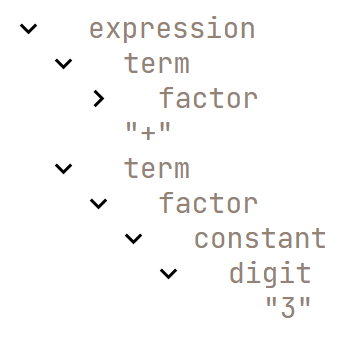
\includegraphics[width=5cm]{parse_tree.png}
  \caption{A screenshot of the visualized parse tree.}
  \label{fig:front-end-parse-tree}
\end{wrapfigure}

Section~\ref{sbs:grammar-processing} described the \texttt{Node} structure,
which represents the parse tree returned from the checker. This structure is
utilized in the visualization of the parse tree on the front-end. Each
\texttt{Node} converted to JavaScript objects is composed of a \texttt{name}
parameter, and, in the case of branch nodes, a \texttt{children} parameter with
an array of all children nodes. This structure is compatible with
\emph{Svelte-tree} package --- a tree-like view component for Svelte. The
component is used on the front-end to display a collapsable tree based on the
structure described above. An example of the visualized parse tree is presented
in figure~\ref{fig:front-end-parse-tree}.

Svelte-tree allows the user to associate a node with an identifier via the
\texttt{let:node} construct, and this way access the names of nodes being
rendered at appropriate DOM elements.

The Svelte-tree is abstracted away into its own Svelte component responsible for
visualizing the parse tree, which can be seen in
listing~\ref{lst:svelte-parse-tree}. In the \texttt{<script>} section it imports
the \texttt{Tree} component from the Svelte-tree package, and exposes the
\texttt{tree} parameter as its input. Each node in the tree is marked with a
\texttt{node} class, which, in the \texttt{<style>} section, is getting an
appropriate styling with CSS.

\begin{listing}[H]
  \begin{minted}[fontsize=\footnotesize,frame=lines,breaklines,linenos]{html}
<script>
  import Tree from "svelte-tree";
  export let tree;
</script>

<main>
  <Tree tree={[tree]} let:node>
    <div class="node">{node.name}</div>
  </Tree>
</main>

<style>
  .node {
    float: left;
    font-family: "JetBrains Mono", Consolas, monospace;
    color: #928374;
    padding-left: 24px;
  }
</style>
  \end{minted}
  \caption{Contents of \texttt{ParseTree.svelte}, the parse tree visualization
  component.}
  \label{lst:svelte-parse-tree}
\end{listing}

\chapter{Project quality study} \label{ch:project-quality-study}

\section{Business logic testing} \label{sec:testing}

\subsection{Unit testing}

\paraphrase{Unit testing is a type of software testing where individual units or
components of a software are tested. The purpose is to validate that each unit
of the software code performs as expected. Unit tests help to fix bugs early in
the development cycle, and help to understand the code base and make changes to
the code quickly. Good unit tests also serve as project documentation. Unit
testing allows the programmer to refactor code at a later date, and make sure
the module still works correctly (i.e. Regression testing). The procedure is to
write test cases for all functions and methods so that whenever a change causes
a fault, it can be quickly identified and fixed. Unit testing, however, can't be
expected to catch every error in a program. It is not possible to evaluate all
execution paths even in the most trivial programs. Unit testing by its very
nature focuses on a unit of code. Hence it can't catch integration errors or
broad system level errors.

A developer writes a section of code in the application just to test the
function. Isolating the tested code helps in revealing unnecessary dependencies
between the code being tested and other units in the project --- testing should
be focused on only one piece of code at a time. Unit Test cases should be
independent. In case of any enhancements or change in requirements, unit test
cases should not be affected. If units are made less interdependent to make unit
testing possible, the unintended impact of changes to any code is less.}

Unit tests in \thisproject{} focus on testing the individual components of the
EBNF parser, that is: the lexer, the parser, and the preprocessor. If the
developer is sure that all of these components work correctly in isolation, the
same thing can be said about the whole system, because there are no hidden
dependencies between these components.

Tests related to the lexer test the functionality of the lexer, that is, test
the ability of the lexer to turn the textual representation of EBNF into
individual tokens. An typical unit test related to the lexer can be seen in
listing~\ref{lst:lexer-unit-test}, where it makes an assertion that the result
of the \texttt{lex} function on input ``\verb*| abc \n = 'def' |'' is a success
(the \texttt{Ok} case), and it's a vector of three certain tokens.

\begin{listing}[H]
  \begin{minted}[fontsize=\scriptsize,frame=lines,breaklines,linenos]{rust}
#[test]
fn test_multiline() {
  assert_eq!(
    lex(" abc \n = 'def' "),
    Ok(vec![
      Token::Nonterminal("abc".to_owned()).spanning(Span::from(((1, 0), (4, 0)))),
      Token::Definition.spanning(Span::from(((1, 1), (2, 1)))),
      Token::Terminal("def".to_owned()).spanning(Span::from(((3, 1), (8, 1))))
    ])
  );
}
  \end{minted}
  \caption{A unit test related to the lexer testing the proper tokenization of
  the input string.}
  \label{lst:lexer-unit-test}
\end{listing}

All test cases related to the lexer are listed in
table~\ref{tab:lexer-test-cases} in a simplified format, where the result can
either be a success case or a failure case, but does not provide information
about the lexed tokens for simplicity. The actual test cases for the lexer
are located in the file \texttt{ebnf/src/lexer/tests.rs}.

\begin{table}[H]
  \centering
  \caption{Tests cases related to the lexer along with the expected results.}
  \label{tab:lexer-test-cases}
  \begin{tabular}{@{}ll@{}}
    \toprule
    Test case & Result \\ \midrule
    \verb*@,@                    & success \\
    \verb*@| /!@                 & success \\
    \verb*@abc = b;@             & success \\
    \verb*@ (/ [ /) ]@           & success \\
    \verb*@ (/) @                & failure \\
    \verb*@ /@                   & success \\
    \verb*@(::) { } @            & success \\
    \verb*@ (:) @                & failure \\
    \verb*@ "ab c " @            & success \\
    \verb*@  '"aba' @            & success \\
    \verb*@ ' a "@               & failure \\
    \verb*@"bbb'   @             & failure \\ \bottomrule
  \end{tabular}
  \hspace{0.5cm}
  \begin{tabular}{@{}ll@{}}
    \toprule
    Test case & Result \\ \midrule
    \verb*@""@                   & failure \\
    \verb*@''@                   & failure \\
    \verb*@ ? test ?@            & success \\
    \verb*@?a\nbc?  @            & success \\
    \verb*@ ?bbb  @              & failure \\
    \verb*@??@                   & success \\
    \verb*@ 123 @                & success \\
    \verb*@ 1 2  3  @            & success \\
    \verb*@ 01234 5@"            & success \\
    \verb*@ 0 @                  & success \\
    \verb*@ abc @                & success \\
    \verb*@a  bc @               & success \\ \bottomrule
  \end{tabular}
  \hspace{0.5cm}
  \begin{tabular}{@{}ll@{}}
    \toprule
    Test case & Result \\ \midrule
    \verb*@abc12 3 @             & success \\
    \verb*@ x @                  & success \\
    \verb*@ + @                  & failure \\
    \verb*@  , \n,@              & success \\
    \verb*@ (* test *) @         & success \\
    \verb*@ (* test * @          & failure \\
    \verb*@ (* (@                & failure \\
    \verb*@, (*, *) , @          & success \\
    \verb*@ ,(*, (* ,*) ,*) , ,@ & success \\
    \verb*@ (* (* *) @           & failure \\
    \verb*@ (*) @                & failure \\
    \verb*@ abc \n = 'def' @     & success \\ \bottomrule
  \end{tabular}
\end{table}

Tests related to the parser test the functionality of the parser, that is, test
the ability to transform a list of tokens into an AST. To make the unit tests of
the parser independent from the implementation of the lexer, the input to the
\texttt{parse} function is a vector of tokens, rather than a result of the
\texttt{lex} function. An example test case related to the parser is seen in
listing~\ref{lst:parser-unit-test}, where the \texttt{ok\_case} macro represents
a test case that, after testing the \texttt{factor} parser, should result in a
success, parse 3 tokens, and return a \texttt{Factor} AST node. In the same
file, that is \texttt{ebnf/src/parser/tests.rs} one can also find the
\texttt{error\_case} macro, which represents a test case that should fail with a
specific error.

\begin{listing}[H]
  \begin{minted}[fontsize=\scriptsize,frame=lines,breaklines,linenos]{rust}
ok_case!(
  factor,
  &vec![
    Token::Integer(2).spanning(Span::from(((0, 0), (1, 0)))),
    Token::Repetition.spanning(Span::from(((2, 0), (3, 0)))),
    Token::Terminal("terminal".to_owned()).spanning(Span::from(((4, 0), (14, 0))))
  ],
  3,
  Expression::Factor {
    count: 2.spanning(Span::from(((0, 0), (1, 0)))),
    primary: Box::new(
      Expression::Terminal("terminal".to_owned()).spanning(Span::from(((4, 0), (14, 0))))
    )
  }
  .spanning(Span::from(((0, 0), (14, 0))))
);
  \end{minted}
  \caption{A unit test related to the parser, where the ability to turn a string
  of tokens into an AST is tested.}
  \label{lst:parser-unit-test}
\end{listing}

Tests related to the preprocessor test the functionality of the preprocessor,
that is, test the ability to detect undefined rules and left recursion. Test
case in listing~\ref{lst:preprocessor-unit-test} tests the grammar
\begin{minted}[fontsize=\small]{lexers/ebnf_lexer.py:EbnfLexer -x}
a = b;
b = a;
\end{minted}
and the detection of indirect left recursion $b \rightarrow a \rightarrow b$.

\begin{listing}[H]
  \begin{minted}[fontsize=\scriptsize,frame=lines,breaklines,linenos]{rust}
#[test]
fn test_indirect_left_recursion() {
  assert_eq!(
    preprocess(
      Grammar {
        productions: vec![
          Production {
            lhs: "a".to_owned().spanning(Span::from(((0, 0), (1, 0)))),
            rhs: Expression::Nonterminal("b".to_owned())
              .spanning(Span::from(((4, 0), (5, 0))))
          }
          .spanning(Span::from(((0, 0), (6, 0)))),
          Production {
            lhs: "b".to_owned().spanning(Span::from(((0, 1), (1, 1)))),
            rhs: Expression::Nonterminal("a".to_owned())
              .spanning(Span::from(((4, 1), (5, 1))))
          }
          .spanning(Span::from(((0, 1), (6, 1))))
        ]
      }
      .spanning(Span::from(((0, 0), (6, 1))))
    ),
    Err(
      Error::LeftRecursion(vec!["b".to_owned(), "a".to_owned(), "b".to_owned()])
        .spanning(Span::from(((4, 0), (5, 0))))
    )
  );
}
  \end{minted}
  \caption{A preprocessor unit test testing the left recursion detection in an
  AST.}
  \label{lst:preprocessor-unit-test}
\end{listing}

All tests related to business logic are written in Rust, as the business logic
is also written in Rust. All unit tests in the project can be ran with the use
of Cargo with the \texttt{cargo test} command in the terminal.

\subsection{Property-based testing}

Test engineers write mostly example-based tests where only one input scenario is
tested. Property-based testing is a useful addition to a test suite because it
runs one statement hundreds of times with different inputs. Property-based
testing frameworks use almost every conceivable input that could break the
code, such as empty lists, negative numbers, and really long lists or strings.
Property based testing has become quite famous in the functional world. Mainly
introduced by QuickCheck framework in Haskell, it suggests another way to test
software.

Property-based tests are designed to test the aspects of a property that should
always be true. They allow for a range of inputs to be programmed and tested
within a single test, rather than having to write a different test for every
value that the programmer wants to test. These tests are useful when a range of
inputs needs to be tested on a given aspect of a software property, or if the
developer is concerned about finding missed edge cases.

\begin{listing}[H]
  \begin{minted}[fontsize=\small,frame=lines,breaklines,linenos]{rust}
use quickcheck_macros::quickcheck;

#[quickcheck]
fn test_arbitrary_input(input: String) {
  let _ = lex(&input);
}
  \end{minted}
  \caption{A QuickCheck test testing arbitrary inputs on the lexer.}
  \label{lst:lexer-quickcheck-test}
\end{listing}

\thisproject{} uses the \texttt{quickcheck} crate for Rust, which is a
property-based testing framework inspired by Haskell's QuickCheck and has been
described in section~\ref{sbs:used-technologies}. \texttt{quickcheck} tests the
``correctness'' of \texttt{lex} and \texttt{parse}, i.e. it checks if these
functions do not emit a \emph{panic} for an arbitrary input, whether it's a
random string of characters for the case of \texttt{lex}, or a random string of
tokens for \texttt{parse}. Example \texttt{quickcheck} tests can be seen in
listings~\ref{lst:lexer-quickcheck-test} and \ref{lst:parser-quickcheck-test},
where the \texttt{quickcheck} macro is used to streamline the usage of the
library. \texttt{quickcheck} catches any panics that may occur in \texttt{lex}
and \texttt{parse} functions and reports them to the user along with the input
provided to these functions. In the case of \texttt{parse}, to generate an
arbitrary string of \texttt{Token}s, it was necessary to implement the
\texttt{Arbitrary} trait provided by \texttt{quickcheck} for \texttt{Token}.
\texttt{Spanned<T>}, \texttt{Span}, and \texttt{Location} types (most of this
has been omitted in listing \ref{lst:parser-quickcheck-test}).

\begin{listing}[H]
  \begin{minted}[fontsize=\small,frame=lines,breaklines,linenos]{rust}
// ...
impl<T: Arbitrary> Arbitrary for Spanned<T> {
  fn arbitrary<G: Gen>(g: &mut G) -> Spanned<T> {
    Spanned {
      node: T::arbitrary(g),
      span: Span::arbitrary(g),
    }
  }
}

#[quickcheck]
fn test_arbitrary_input(tokens: Vec<Spanned<Token>>) {
    use super::parse;
    let _ = parse(tokens.as_slice());
}
  \end{minted}
  \caption{A QuickCheck test related to the parser, testing strings of arbitrary
  tokens.}
  \label{lst:parser-quickcheck-test}
\end{listing}

\section{Integration testing}

Integration testing is defined as a type of testing where software modules are
integrated logically and tested as a group. A typical software project consists
of multiple software modules, coded by different programmers. The purpose of
this level of testing is to expose defects in the interaction between these
software modules when they are integrated.

\thisproject{} utilizes integration testing thanks to \emph{wasm-pack}. This
tool allows the developer you build rust-generated WebAssembly packages, as well
as test them in a headless web browser via the wasm-pack test command. A tool
used to define the integration tests is the wasm-bindgen-test crate --- an
experimental test harness for Rust programs compiled to wasm using wasm-bindgen
and the wasm32-unknown-unknown target. The \texttt{wasm-pack test} command wraps
the wasm-bindgen-test-runner CLI allowing the developer to run wasm tests in
different browsers without needing to install the different webdrivers. An
example integration test ran with wasm-bindgen-test can be seen in
listing~\ref{lst:ebnf-integration-tests}.

\begin{listing}[H]
  \begin{minted}[fontsize=\small,frame=lines,breaklines,linenos]{rust}
use ebnf::parse;
use wasm_bindgen_test::*;

#[wasm_bindgen_test]
fn test_ebnf() {
  assert!(parse(" abc = 'def'; ").is_ok());
  assert!(parse(" (* test *) ").is_err());
  assert!(parse(" (* test *").is_err());
  assert!(parse("a = b;").is_err());
  assert!(parse("a = 'a';;").is_err());
  assert!(parse("a = ;").is_ok());
  assert!(parse("a = a;").is_err());
}
  \end{minted}
  \caption{An integration test ran in a headless browser, which tests various
  grammars in a textual form.}
  \label{lst:ebnf-integration-tests}
\end{listing}

\section{Benchmarking}

Benchmarks check the performance of the code. \thisproject{}'s benchmark tool of
choice is Criterion.rs --- a statistics-driven micro-benchmarking tool. It is a
Rust port of Haskell's Criterion library. Criterion.rs benchmarks collect and
store statistical information from run to run and can automatically detect
performance regressions as well as measuring optimizations.
Listing~\ref{lst:benchmark} shows a Criterion.rs benchmark that parses a sample
input grammar multiple times.

\begin{listing}[H]
  \begin{minted}[fontsize=\footnotesize,frame=lines,breaklines,linenos]{rust}
use criterion::{black_box, criterion_group, criterion_main, Criterion};
use ebnf::parse;

const GRAMMAR: &str = "
expression = term, { ('+' | '-'), term };
term       = factor, { ('*' | '/'), factor };
factor     = constant | variable | '(', expression, ')';
variable   = 'x' | 'y' | 'z';
constant   = digit, { digit };
digit      = '0' | '1' | '2' | '3' | '4' | '5' | '6' | '7' | '8' | '9';
";

fn criterion_benchmark(c: &mut Criterion) {
  c.bench_function("parse", |b| b.iter(|| parse(black_box(GRAMMAR))));
}

criterion_group!(benches, criterion_benchmark);
criterion_main!(benches);
  \end{minted}
  \caption{A benchmark testing the speed of parsing a sample grammar.}
  \label{lst:benchmark}
\end{listing}

Criterion.rs can generate a number of useful charts and graphs which the
developer can check to get a better understanding of the behavior of the
benchmark. These charts will be generated with \emph{gnuplot} by default, and
the examples below were generated using the gnuplot backend.

\begin{figure}[H]
  \centering
  \resizebox{\textwidth}{!}{\footnotesize\input{images/pdf_bench.pdf_tex}}
  \caption{Probability Distribution Function chart generated by Criterion.rs.}
  \label{fig:pdf-benchmark}
\end{figure}

The \emph{PDF chart} in figure~\ref{fig:pdf-benchmark} shows the
\emph{probability distribution function} for the samples. It also shows the
ranges used to classify samples as outliers. In this example we can see that the
performance trend does not change noticeably across the whole benchmark and
stays around \SI{55}{\micro\second}

\begin{figure}[H]
  \centering
  \resizebox{\textwidth}{!}{\footnotesize\input{images/regression_bench.pdf_tex}}
  \caption{Regression plot generated by Criterion.rs.}
  \label{fig:regression-benchmark}
\end{figure}

The \emph{regression plot}, shown in figure~\ref{fig:regression-benchmark},
shows each data point plotted on an X-Y plane showing the number of iterations
versus the time taken. It also shows the line representing Criterion.rs' best
guess at the time per iteration. A good benchmark will show the data points all
closely following the line. If the data points are scattered widely, this
indicates that there is a lot of noise in the data and that the benchmark may
not be reliable. If the data points follow a consistent trend but don't match
the line (eg. if they follow a curved pattern or show several discrete line
segments) this indicates that the benchmark is doing different amounts of work
depending on the number of iterations, which prevents Criterion.rs from
generating accurate statistics and means that the benchmark may need to be
reworked.

The graphics that Criterion.rs generates are perfect for contributors of the
project as there is no dearth of info. Criterion generates graphics that break
down mean, median, standard deviation, MAD, etc., which are invaluable when
trying to pinpoint areas of improvement.

\section{Auditing}

A software audit is an internal or external review of a software program to
check its quality, progress or adherence to plans, standards and regulations.
\thisproject{} utilizes Google Lighthouse --- an open-source, automated tool for
improving the quality of web pages. Developers can run it against any web page,
public or requiring authentication. It has audits for performance,
accessibility, progressive web apps, SEO and more. When the tool finishes
analyzing a web page, it returns a report with the calculated scores for each
metric, a list of problems with the page, and general, or sometimes specific,
recommendations regarding solving those problems.
Figure~\ref{fig:lighthouse-summary} shows a short summary of Lighthouse ran
against the deployed web application. For most metrics, Lighthouse calculates a
score by comparing the page with the FCP data present in HTTP Archive. The tool
uses a color-coding system to display how well a page performs according to a
particular metric.

\begin{figure}[h]
  \centering
  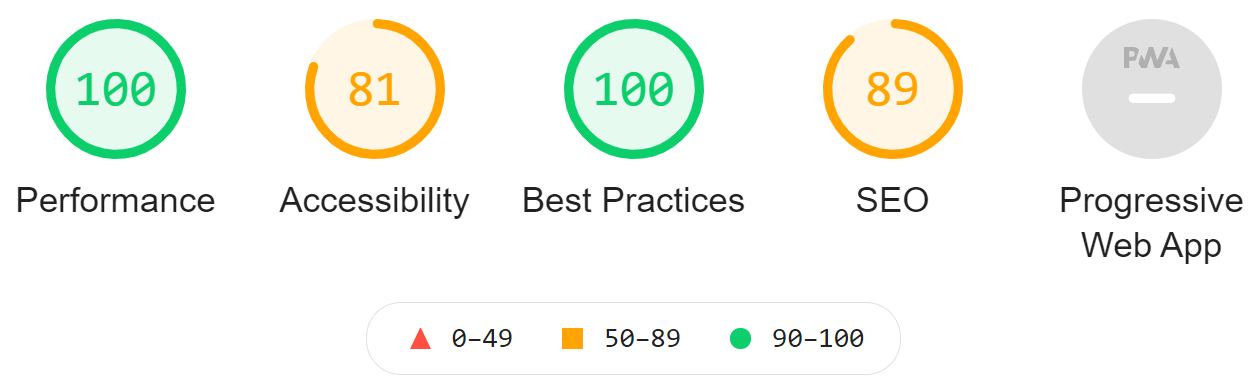
\includegraphics[width=\textwidth]{lighthouse_summary.png}
  \caption{Google Lighthouse's scores of the deployed web application.}
  \label{fig:lighthouse-summary}
\end{figure}

\thisproject{} scores 100 points in the performance category. This category has
metrics that together reflect how fast the page is perceptually:
\begin{description}
  \item[First Contentful Paint] Shows how long it takes for a browser to render
  DOM content,
  \item[Speed Index] Shows how quickly the contents of a page load visually. To
  do this, Lighthouse records a video of your page loading and then computes a
  visual progression between frames,
  \item[Largest Contentful Paint] Reports the render time of the largest image
  or text block within the viewport (i.e., the visible part of the page),
  \item[Time To Interactive] Measures how long it takes a page to become
  \emph{fully} interactive, i.e. useful content (measured by FCP) is displayed,
  JavaScript event handlers are bound to visible elements' events, and the page
  responds to user interaction within 50 milliseconds,
  \item[Total Blocking Time] The sum of all time records between FCP and TTI
  when a page is blocked from user interaction for more than 50 milliseconds,
  \item[Cumulative Layout Shift] Metric for showing how aggressively elements
  shift each other during the loading.
\end{description}
All values for performance metrics generated by Lighthouse can be seen in
table~\ref{tab:lighthouse-performance-metrics}. Besides the metrics, the website
passed additional 29 audits, such as \emph{Minify CSS}, \emph{Minify
JavaScript}, \emph{Enable text compression}, \emph{Initial server response time
was short}, \emph{Remove duplicate modules in JavaScript bundles}, \emph{Avoids
an excessive DOM size} and more.
\begin{table}[H]
  \centering
  \caption{Performance metrics generated by Lighthouse.}
  \label{tab:lighthouse-performance-metrics}
  \begin{tabular}{@{}lr@{}}
    \toprule
    Metric                   & Value                 \\ \midrule
    First Contentful Paint   & \SI{0.2}{\second}     \\
    Speed Index              & \SI{0.4}{\second}     \\
    Largest Contentful Paint & \SI{0.4}{\second}     \\
    Time to Interactive      & \SI{0.4}{\second}     \\
    Total Blocking Time      & \SI{0}{\milli\second} \\
    Cumulative Layout Shift  & 0                     \\ \bottomrule
  \end{tabular}
\end{table}

In terms of best practices, the web application scores 100 points, thanks to
HTTPS usage provided by GitHub Pages, safe links to cross-origin destinations,
avoiding requesting geolocation and notification permissions on page load,
and avoiding front-end JavaScript libraries with known security vulnerabilities.

Besides performance audits, Lighthouse also provides audits regarding
accessibility, SEO (Search Engine Optimization), and PWA (Progressive Web App).
These audits were not the main focus of the project, however they provide useful
information about possible future improvements. Lighthouse informs that
background and foreground colors do not have a sufficient contrast ratio and
that low-contrast text is difficult or impossible for many users to read, which
is a valid concern that should be taken into consideration. The accessibility
audit also suggests providing labels for associated form elements, which most
likely relates to \texttt{textarea} grammar and input string fields. In terms of
Progressive Web App audits, Lighthouse suggests using a service worker, which
enables the web app to be reliable in unpredictable network conditions and use
many Progressive Web App features, such as \emph{offline}, \emph{add to
homescreen}, and \emph{push notifications}.

\newpage

\section{Complexity analysis}

Software complexity is a way to describe a specific set of characteristics of
the code. These characteristics all focus on how the code interacts with other
pieces of code.

A popular metric for measuring code complexity is \emph{cyclomatic complexity}.
Cyclomatic complexity uses a mathematical model to assess methods, producing
accurate measurements of the effort required to test them, but inaccurate
measurements of the effort required to understand them.

\emph{Cognitive complexity}, on the other hand, breaks from the practice of
using mathematical models to assess software maintainability. It starts from the
precedents set by cyclomatic complexity, but uses human judgement to assess how
structures should be counted, and to decide what should be added to the model as
a whole. As a result, it yields method complexity scores which strike
programmers as fairer relative assessments of maintainability than have been
available with previous models.

Calculating cognitive complexity in Rust can be achieved with the
\emph{rust-clippy} tool. Clippy is a collection of lints to catch common
mistakes and improve Rust code. There are over 400 lints included in the tool,
and are divided into categories, each with a default lint level. One way to use
Clippy is by installing Clippy through \texttt{rustup} as a Cargo subcommand.
Clippy can then be invoked with the \texttt{cargo clippy} command.

\begin{figure}[H]
  \centering
  %% Creator: Matplotlib, PGF backend
%%
%% To include the figure in your LaTeX document, write
%%   \input{<filename>.pgf}
%%
%% Make sure the required packages are loaded in your preamble
%%   \usepackage{pgf}
%%
%% and, on pdftex
%%   \usepackage[utf8]{inputenc}\DeclareUnicodeCharacter{2212}{-}
%%
%% or, on luatex and xetex
%%   \usepackage{unicode-math}
%%
%% Figures using additional raster images can only be included by \input if
%% they are in the same directory as the main LaTeX file. For loading figures
%% from other directories you can use the `import` package
%%   \usepackage{import}
%%
%% and then include the figures with
%%   \import{<path to file>}{<filename>.pgf}
%%
%% Matplotlib used the following preamble
%%
\begingroup%
\makeatletter%
\begin{pgfpicture}%
\pgfpathrectangle{\pgfpointorigin}{\pgfqpoint{6.000000in}{2.500000in}}%
\pgfusepath{use as bounding box, clip}%
\begin{pgfscope}%
\pgfsetbuttcap%
\pgfsetmiterjoin%
\pgfsetlinewidth{0.000000pt}%
\definecolor{currentstroke}{rgb}{1.000000,1.000000,1.000000}%
\pgfsetstrokecolor{currentstroke}%
\pgfsetstrokeopacity{0.000000}%
\pgfsetdash{}{0pt}%
\pgfpathmoveto{\pgfqpoint{0.000000in}{0.000000in}}%
\pgfpathlineto{\pgfqpoint{6.000000in}{0.000000in}}%
\pgfpathlineto{\pgfqpoint{6.000000in}{2.500000in}}%
\pgfpathlineto{\pgfqpoint{0.000000in}{2.500000in}}%
\pgfpathclose%
\pgfusepath{}%
\end{pgfscope}%
\begin{pgfscope}%
\pgfsetbuttcap%
\pgfsetmiterjoin%
\definecolor{currentfill}{rgb}{1.000000,1.000000,1.000000}%
\pgfsetfillcolor{currentfill}%
\pgfsetlinewidth{0.000000pt}%
\definecolor{currentstroke}{rgb}{0.000000,0.000000,0.000000}%
\pgfsetstrokecolor{currentstroke}%
\pgfsetstrokeopacity{0.000000}%
\pgfsetdash{}{0pt}%
\pgfpathmoveto{\pgfqpoint{0.600000in}{0.450000in}}%
\pgfpathlineto{\pgfqpoint{5.400000in}{0.450000in}}%
\pgfpathlineto{\pgfqpoint{5.400000in}{2.487500in}}%
\pgfpathlineto{\pgfqpoint{0.600000in}{2.487500in}}%
\pgfpathclose%
\pgfusepath{fill}%
\end{pgfscope}%
\begin{pgfscope}%
\pgfpathrectangle{\pgfqpoint{0.600000in}{0.450000in}}{\pgfqpoint{4.800000in}{2.037500in}}%
\pgfusepath{clip}%
\pgfsetbuttcap%
\pgfsetmiterjoin%
\definecolor{currentfill}{rgb}{0.121569,0.466667,0.705882}%
\pgfsetfillcolor{currentfill}%
\pgfsetlinewidth{0.000000pt}%
\definecolor{currentstroke}{rgb}{0.000000,0.000000,0.000000}%
\pgfsetstrokecolor{currentstroke}%
\pgfsetstrokeopacity{0.000000}%
\pgfsetdash{}{0pt}%
\pgfpathmoveto{\pgfqpoint{0.818182in}{0.450000in}}%
\pgfpathlineto{\pgfqpoint{1.003868in}{0.450000in}}%
\pgfpathlineto{\pgfqpoint{1.003868in}{2.390476in}}%
\pgfpathlineto{\pgfqpoint{0.818182in}{2.390476in}}%
\pgfpathclose%
\pgfusepath{fill}%
\end{pgfscope}%
\begin{pgfscope}%
\pgfpathrectangle{\pgfqpoint{0.600000in}{0.450000in}}{\pgfqpoint{4.800000in}{2.037500in}}%
\pgfusepath{clip}%
\pgfsetbuttcap%
\pgfsetmiterjoin%
\definecolor{currentfill}{rgb}{0.121569,0.466667,0.705882}%
\pgfsetfillcolor{currentfill}%
\pgfsetlinewidth{0.000000pt}%
\definecolor{currentstroke}{rgb}{0.000000,0.000000,0.000000}%
\pgfsetstrokecolor{currentstroke}%
\pgfsetstrokeopacity{0.000000}%
\pgfsetdash{}{0pt}%
\pgfpathmoveto{\pgfqpoint{1.050290in}{0.450000in}}%
\pgfpathlineto{\pgfqpoint{1.235977in}{0.450000in}}%
\pgfpathlineto{\pgfqpoint{1.235977in}{1.454889in}}%
\pgfpathlineto{\pgfqpoint{1.050290in}{1.454889in}}%
\pgfpathclose%
\pgfusepath{fill}%
\end{pgfscope}%
\begin{pgfscope}%
\pgfpathrectangle{\pgfqpoint{0.600000in}{0.450000in}}{\pgfqpoint{4.800000in}{2.037500in}}%
\pgfusepath{clip}%
\pgfsetbuttcap%
\pgfsetmiterjoin%
\definecolor{currentfill}{rgb}{0.121569,0.466667,0.705882}%
\pgfsetfillcolor{currentfill}%
\pgfsetlinewidth{0.000000pt}%
\definecolor{currentstroke}{rgb}{0.000000,0.000000,0.000000}%
\pgfsetstrokecolor{currentstroke}%
\pgfsetstrokeopacity{0.000000}%
\pgfsetdash{}{0pt}%
\pgfpathmoveto{\pgfqpoint{1.282398in}{0.450000in}}%
\pgfpathlineto{\pgfqpoint{1.468085in}{0.450000in}}%
\pgfpathlineto{\pgfqpoint{1.468085in}{0.588605in}}%
\pgfpathlineto{\pgfqpoint{1.282398in}{0.588605in}}%
\pgfpathclose%
\pgfusepath{fill}%
\end{pgfscope}%
\begin{pgfscope}%
\pgfpathrectangle{\pgfqpoint{0.600000in}{0.450000in}}{\pgfqpoint{4.800000in}{2.037500in}}%
\pgfusepath{clip}%
\pgfsetbuttcap%
\pgfsetmiterjoin%
\definecolor{currentfill}{rgb}{0.121569,0.466667,0.705882}%
\pgfsetfillcolor{currentfill}%
\pgfsetlinewidth{0.000000pt}%
\definecolor{currentstroke}{rgb}{0.000000,0.000000,0.000000}%
\pgfsetstrokecolor{currentstroke}%
\pgfsetstrokeopacity{0.000000}%
\pgfsetdash{}{0pt}%
\pgfpathmoveto{\pgfqpoint{1.514507in}{0.450000in}}%
\pgfpathlineto{\pgfqpoint{1.700193in}{0.450000in}}%
\pgfpathlineto{\pgfqpoint{1.700193in}{0.484651in}}%
\pgfpathlineto{\pgfqpoint{1.514507in}{0.484651in}}%
\pgfpathclose%
\pgfusepath{fill}%
\end{pgfscope}%
\begin{pgfscope}%
\pgfpathrectangle{\pgfqpoint{0.600000in}{0.450000in}}{\pgfqpoint{4.800000in}{2.037500in}}%
\pgfusepath{clip}%
\pgfsetbuttcap%
\pgfsetmiterjoin%
\definecolor{currentfill}{rgb}{0.121569,0.466667,0.705882}%
\pgfsetfillcolor{currentfill}%
\pgfsetlinewidth{0.000000pt}%
\definecolor{currentstroke}{rgb}{0.000000,0.000000,0.000000}%
\pgfsetstrokecolor{currentstroke}%
\pgfsetstrokeopacity{0.000000}%
\pgfsetdash{}{0pt}%
\pgfpathmoveto{\pgfqpoint{1.746615in}{0.450000in}}%
\pgfpathlineto{\pgfqpoint{1.932302in}{0.450000in}}%
\pgfpathlineto{\pgfqpoint{1.932302in}{0.519303in}}%
\pgfpathlineto{\pgfqpoint{1.746615in}{0.519303in}}%
\pgfpathclose%
\pgfusepath{fill}%
\end{pgfscope}%
\begin{pgfscope}%
\pgfpathrectangle{\pgfqpoint{0.600000in}{0.450000in}}{\pgfqpoint{4.800000in}{2.037500in}}%
\pgfusepath{clip}%
\pgfsetbuttcap%
\pgfsetmiterjoin%
\definecolor{currentfill}{rgb}{0.121569,0.466667,0.705882}%
\pgfsetfillcolor{currentfill}%
\pgfsetlinewidth{0.000000pt}%
\definecolor{currentstroke}{rgb}{0.000000,0.000000,0.000000}%
\pgfsetstrokecolor{currentstroke}%
\pgfsetstrokeopacity{0.000000}%
\pgfsetdash{}{0pt}%
\pgfpathmoveto{\pgfqpoint{1.978723in}{0.450000in}}%
\pgfpathlineto{\pgfqpoint{2.164410in}{0.450000in}}%
\pgfpathlineto{\pgfqpoint{2.164410in}{0.519303in}}%
\pgfpathlineto{\pgfqpoint{1.978723in}{0.519303in}}%
\pgfpathclose%
\pgfusepath{fill}%
\end{pgfscope}%
\begin{pgfscope}%
\pgfpathrectangle{\pgfqpoint{0.600000in}{0.450000in}}{\pgfqpoint{4.800000in}{2.037500in}}%
\pgfusepath{clip}%
\pgfsetbuttcap%
\pgfsetmiterjoin%
\definecolor{currentfill}{rgb}{0.121569,0.466667,0.705882}%
\pgfsetfillcolor{currentfill}%
\pgfsetlinewidth{0.000000pt}%
\definecolor{currentstroke}{rgb}{0.000000,0.000000,0.000000}%
\pgfsetstrokecolor{currentstroke}%
\pgfsetstrokeopacity{0.000000}%
\pgfsetdash{}{0pt}%
\pgfpathmoveto{\pgfqpoint{2.210832in}{0.450000in}}%
\pgfpathlineto{\pgfqpoint{2.396518in}{0.450000in}}%
\pgfpathlineto{\pgfqpoint{2.396518in}{0.450000in}}%
\pgfpathlineto{\pgfqpoint{2.210832in}{0.450000in}}%
\pgfpathclose%
\pgfusepath{fill}%
\end{pgfscope}%
\begin{pgfscope}%
\pgfpathrectangle{\pgfqpoint{0.600000in}{0.450000in}}{\pgfqpoint{4.800000in}{2.037500in}}%
\pgfusepath{clip}%
\pgfsetbuttcap%
\pgfsetmiterjoin%
\definecolor{currentfill}{rgb}{0.121569,0.466667,0.705882}%
\pgfsetfillcolor{currentfill}%
\pgfsetlinewidth{0.000000pt}%
\definecolor{currentstroke}{rgb}{0.000000,0.000000,0.000000}%
\pgfsetstrokecolor{currentstroke}%
\pgfsetstrokeopacity{0.000000}%
\pgfsetdash{}{0pt}%
\pgfpathmoveto{\pgfqpoint{2.442940in}{0.450000in}}%
\pgfpathlineto{\pgfqpoint{2.628627in}{0.450000in}}%
\pgfpathlineto{\pgfqpoint{2.628627in}{0.450000in}}%
\pgfpathlineto{\pgfqpoint{2.442940in}{0.450000in}}%
\pgfpathclose%
\pgfusepath{fill}%
\end{pgfscope}%
\begin{pgfscope}%
\pgfpathrectangle{\pgfqpoint{0.600000in}{0.450000in}}{\pgfqpoint{4.800000in}{2.037500in}}%
\pgfusepath{clip}%
\pgfsetbuttcap%
\pgfsetmiterjoin%
\definecolor{currentfill}{rgb}{0.121569,0.466667,0.705882}%
\pgfsetfillcolor{currentfill}%
\pgfsetlinewidth{0.000000pt}%
\definecolor{currentstroke}{rgb}{0.000000,0.000000,0.000000}%
\pgfsetstrokecolor{currentstroke}%
\pgfsetstrokeopacity{0.000000}%
\pgfsetdash{}{0pt}%
\pgfpathmoveto{\pgfqpoint{2.675048in}{0.450000in}}%
\pgfpathlineto{\pgfqpoint{2.860735in}{0.450000in}}%
\pgfpathlineto{\pgfqpoint{2.860735in}{0.484651in}}%
\pgfpathlineto{\pgfqpoint{2.675048in}{0.484651in}}%
\pgfpathclose%
\pgfusepath{fill}%
\end{pgfscope}%
\begin{pgfscope}%
\pgfpathrectangle{\pgfqpoint{0.600000in}{0.450000in}}{\pgfqpoint{4.800000in}{2.037500in}}%
\pgfusepath{clip}%
\pgfsetbuttcap%
\pgfsetmiterjoin%
\definecolor{currentfill}{rgb}{0.121569,0.466667,0.705882}%
\pgfsetfillcolor{currentfill}%
\pgfsetlinewidth{0.000000pt}%
\definecolor{currentstroke}{rgb}{0.000000,0.000000,0.000000}%
\pgfsetstrokecolor{currentstroke}%
\pgfsetstrokeopacity{0.000000}%
\pgfsetdash{}{0pt}%
\pgfpathmoveto{\pgfqpoint{2.907157in}{0.450000in}}%
\pgfpathlineto{\pgfqpoint{3.092843in}{0.450000in}}%
\pgfpathlineto{\pgfqpoint{3.092843in}{0.450000in}}%
\pgfpathlineto{\pgfqpoint{2.907157in}{0.450000in}}%
\pgfpathclose%
\pgfusepath{fill}%
\end{pgfscope}%
\begin{pgfscope}%
\pgfpathrectangle{\pgfqpoint{0.600000in}{0.450000in}}{\pgfqpoint{4.800000in}{2.037500in}}%
\pgfusepath{clip}%
\pgfsetbuttcap%
\pgfsetmiterjoin%
\definecolor{currentfill}{rgb}{0.121569,0.466667,0.705882}%
\pgfsetfillcolor{currentfill}%
\pgfsetlinewidth{0.000000pt}%
\definecolor{currentstroke}{rgb}{0.000000,0.000000,0.000000}%
\pgfsetstrokecolor{currentstroke}%
\pgfsetstrokeopacity{0.000000}%
\pgfsetdash{}{0pt}%
\pgfpathmoveto{\pgfqpoint{3.139265in}{0.450000in}}%
\pgfpathlineto{\pgfqpoint{3.324952in}{0.450000in}}%
\pgfpathlineto{\pgfqpoint{3.324952in}{0.450000in}}%
\pgfpathlineto{\pgfqpoint{3.139265in}{0.450000in}}%
\pgfpathclose%
\pgfusepath{fill}%
\end{pgfscope}%
\begin{pgfscope}%
\pgfpathrectangle{\pgfqpoint{0.600000in}{0.450000in}}{\pgfqpoint{4.800000in}{2.037500in}}%
\pgfusepath{clip}%
\pgfsetbuttcap%
\pgfsetmiterjoin%
\definecolor{currentfill}{rgb}{0.121569,0.466667,0.705882}%
\pgfsetfillcolor{currentfill}%
\pgfsetlinewidth{0.000000pt}%
\definecolor{currentstroke}{rgb}{0.000000,0.000000,0.000000}%
\pgfsetstrokecolor{currentstroke}%
\pgfsetstrokeopacity{0.000000}%
\pgfsetdash{}{0pt}%
\pgfpathmoveto{\pgfqpoint{3.371373in}{0.450000in}}%
\pgfpathlineto{\pgfqpoint{3.557060in}{0.450000in}}%
\pgfpathlineto{\pgfqpoint{3.557060in}{0.450000in}}%
\pgfpathlineto{\pgfqpoint{3.371373in}{0.450000in}}%
\pgfpathclose%
\pgfusepath{fill}%
\end{pgfscope}%
\begin{pgfscope}%
\pgfpathrectangle{\pgfqpoint{0.600000in}{0.450000in}}{\pgfqpoint{4.800000in}{2.037500in}}%
\pgfusepath{clip}%
\pgfsetbuttcap%
\pgfsetmiterjoin%
\definecolor{currentfill}{rgb}{0.121569,0.466667,0.705882}%
\pgfsetfillcolor{currentfill}%
\pgfsetlinewidth{0.000000pt}%
\definecolor{currentstroke}{rgb}{0.000000,0.000000,0.000000}%
\pgfsetstrokecolor{currentstroke}%
\pgfsetstrokeopacity{0.000000}%
\pgfsetdash{}{0pt}%
\pgfpathmoveto{\pgfqpoint{3.603482in}{0.450000in}}%
\pgfpathlineto{\pgfqpoint{3.789168in}{0.450000in}}%
\pgfpathlineto{\pgfqpoint{3.789168in}{0.450000in}}%
\pgfpathlineto{\pgfqpoint{3.603482in}{0.450000in}}%
\pgfpathclose%
\pgfusepath{fill}%
\end{pgfscope}%
\begin{pgfscope}%
\pgfpathrectangle{\pgfqpoint{0.600000in}{0.450000in}}{\pgfqpoint{4.800000in}{2.037500in}}%
\pgfusepath{clip}%
\pgfsetbuttcap%
\pgfsetmiterjoin%
\definecolor{currentfill}{rgb}{0.121569,0.466667,0.705882}%
\pgfsetfillcolor{currentfill}%
\pgfsetlinewidth{0.000000pt}%
\definecolor{currentstroke}{rgb}{0.000000,0.000000,0.000000}%
\pgfsetstrokecolor{currentstroke}%
\pgfsetstrokeopacity{0.000000}%
\pgfsetdash{}{0pt}%
\pgfpathmoveto{\pgfqpoint{3.835590in}{0.450000in}}%
\pgfpathlineto{\pgfqpoint{4.021277in}{0.450000in}}%
\pgfpathlineto{\pgfqpoint{4.021277in}{0.450000in}}%
\pgfpathlineto{\pgfqpoint{3.835590in}{0.450000in}}%
\pgfpathclose%
\pgfusepath{fill}%
\end{pgfscope}%
\begin{pgfscope}%
\pgfpathrectangle{\pgfqpoint{0.600000in}{0.450000in}}{\pgfqpoint{4.800000in}{2.037500in}}%
\pgfusepath{clip}%
\pgfsetbuttcap%
\pgfsetmiterjoin%
\definecolor{currentfill}{rgb}{0.121569,0.466667,0.705882}%
\pgfsetfillcolor{currentfill}%
\pgfsetlinewidth{0.000000pt}%
\definecolor{currentstroke}{rgb}{0.000000,0.000000,0.000000}%
\pgfsetstrokecolor{currentstroke}%
\pgfsetstrokeopacity{0.000000}%
\pgfsetdash{}{0pt}%
\pgfpathmoveto{\pgfqpoint{4.067698in}{0.450000in}}%
\pgfpathlineto{\pgfqpoint{4.253385in}{0.450000in}}%
\pgfpathlineto{\pgfqpoint{4.253385in}{0.450000in}}%
\pgfpathlineto{\pgfqpoint{4.067698in}{0.450000in}}%
\pgfpathclose%
\pgfusepath{fill}%
\end{pgfscope}%
\begin{pgfscope}%
\pgfpathrectangle{\pgfqpoint{0.600000in}{0.450000in}}{\pgfqpoint{4.800000in}{2.037500in}}%
\pgfusepath{clip}%
\pgfsetbuttcap%
\pgfsetmiterjoin%
\definecolor{currentfill}{rgb}{0.121569,0.466667,0.705882}%
\pgfsetfillcolor{currentfill}%
\pgfsetlinewidth{0.000000pt}%
\definecolor{currentstroke}{rgb}{0.000000,0.000000,0.000000}%
\pgfsetstrokecolor{currentstroke}%
\pgfsetstrokeopacity{0.000000}%
\pgfsetdash{}{0pt}%
\pgfpathmoveto{\pgfqpoint{4.299807in}{0.450000in}}%
\pgfpathlineto{\pgfqpoint{4.485493in}{0.450000in}}%
\pgfpathlineto{\pgfqpoint{4.485493in}{0.450000in}}%
\pgfpathlineto{\pgfqpoint{4.299807in}{0.450000in}}%
\pgfpathclose%
\pgfusepath{fill}%
\end{pgfscope}%
\begin{pgfscope}%
\pgfpathrectangle{\pgfqpoint{0.600000in}{0.450000in}}{\pgfqpoint{4.800000in}{2.037500in}}%
\pgfusepath{clip}%
\pgfsetbuttcap%
\pgfsetmiterjoin%
\definecolor{currentfill}{rgb}{0.121569,0.466667,0.705882}%
\pgfsetfillcolor{currentfill}%
\pgfsetlinewidth{0.000000pt}%
\definecolor{currentstroke}{rgb}{0.000000,0.000000,0.000000}%
\pgfsetstrokecolor{currentstroke}%
\pgfsetstrokeopacity{0.000000}%
\pgfsetdash{}{0pt}%
\pgfpathmoveto{\pgfqpoint{4.531915in}{0.450000in}}%
\pgfpathlineto{\pgfqpoint{4.717602in}{0.450000in}}%
\pgfpathlineto{\pgfqpoint{4.717602in}{0.450000in}}%
\pgfpathlineto{\pgfqpoint{4.531915in}{0.450000in}}%
\pgfpathclose%
\pgfusepath{fill}%
\end{pgfscope}%
\begin{pgfscope}%
\pgfpathrectangle{\pgfqpoint{0.600000in}{0.450000in}}{\pgfqpoint{4.800000in}{2.037500in}}%
\pgfusepath{clip}%
\pgfsetbuttcap%
\pgfsetmiterjoin%
\definecolor{currentfill}{rgb}{0.121569,0.466667,0.705882}%
\pgfsetfillcolor{currentfill}%
\pgfsetlinewidth{0.000000pt}%
\definecolor{currentstroke}{rgb}{0.000000,0.000000,0.000000}%
\pgfsetstrokecolor{currentstroke}%
\pgfsetstrokeopacity{0.000000}%
\pgfsetdash{}{0pt}%
\pgfpathmoveto{\pgfqpoint{4.764023in}{0.450000in}}%
\pgfpathlineto{\pgfqpoint{4.949710in}{0.450000in}}%
\pgfpathlineto{\pgfqpoint{4.949710in}{0.450000in}}%
\pgfpathlineto{\pgfqpoint{4.764023in}{0.450000in}}%
\pgfpathclose%
\pgfusepath{fill}%
\end{pgfscope}%
\begin{pgfscope}%
\pgfpathrectangle{\pgfqpoint{0.600000in}{0.450000in}}{\pgfqpoint{4.800000in}{2.037500in}}%
\pgfusepath{clip}%
\pgfsetbuttcap%
\pgfsetmiterjoin%
\definecolor{currentfill}{rgb}{0.121569,0.466667,0.705882}%
\pgfsetfillcolor{currentfill}%
\pgfsetlinewidth{0.000000pt}%
\definecolor{currentstroke}{rgb}{0.000000,0.000000,0.000000}%
\pgfsetstrokecolor{currentstroke}%
\pgfsetstrokeopacity{0.000000}%
\pgfsetdash{}{0pt}%
\pgfpathmoveto{\pgfqpoint{4.996132in}{0.450000in}}%
\pgfpathlineto{\pgfqpoint{5.181818in}{0.450000in}}%
\pgfpathlineto{\pgfqpoint{5.181818in}{0.484651in}}%
\pgfpathlineto{\pgfqpoint{4.996132in}{0.484651in}}%
\pgfpathclose%
\pgfusepath{fill}%
\end{pgfscope}%
\begin{pgfscope}%
\pgfsetbuttcap%
\pgfsetroundjoin%
\definecolor{currentfill}{rgb}{0.000000,0.000000,0.000000}%
\pgfsetfillcolor{currentfill}%
\pgfsetlinewidth{0.803000pt}%
\definecolor{currentstroke}{rgb}{0.000000,0.000000,0.000000}%
\pgfsetstrokecolor{currentstroke}%
\pgfsetdash{}{0pt}%
\pgfsys@defobject{currentmarker}{\pgfqpoint{0.000000in}{-0.048611in}}{\pgfqpoint{0.000000in}{0.000000in}}{%
\pgfpathmoveto{\pgfqpoint{0.000000in}{0.000000in}}%
\pgfpathlineto{\pgfqpoint{0.000000in}{-0.048611in}}%
\pgfusepath{stroke,fill}%
}%
\begin{pgfscope}%
\pgfsys@transformshift{0.911025in}{0.450000in}%
\pgfsys@useobject{currentmarker}{}%
\end{pgfscope}%
\end{pgfscope}%
\begin{pgfscope}%
\definecolor{textcolor}{rgb}{0.000000,0.000000,0.000000}%
\pgfsetstrokecolor{textcolor}%
\pgfsetfillcolor{textcolor}%
\pgftext[x=0.911025in,y=0.352778in,,top]{\color{textcolor}\rmfamily\fontsize{10.000000}{12.000000}\selectfont \(\displaystyle {1}\)}%
\end{pgfscope}%
\begin{pgfscope}%
\pgfsetbuttcap%
\pgfsetroundjoin%
\definecolor{currentfill}{rgb}{0.000000,0.000000,0.000000}%
\pgfsetfillcolor{currentfill}%
\pgfsetlinewidth{0.803000pt}%
\definecolor{currentstroke}{rgb}{0.000000,0.000000,0.000000}%
\pgfsetstrokecolor{currentstroke}%
\pgfsetdash{}{0pt}%
\pgfsys@defobject{currentmarker}{\pgfqpoint{0.000000in}{-0.048611in}}{\pgfqpoint{0.000000in}{0.000000in}}{%
\pgfpathmoveto{\pgfqpoint{0.000000in}{0.000000in}}%
\pgfpathlineto{\pgfqpoint{0.000000in}{-0.048611in}}%
\pgfusepath{stroke,fill}%
}%
\begin{pgfscope}%
\pgfsys@transformshift{1.143133in}{0.450000in}%
\pgfsys@useobject{currentmarker}{}%
\end{pgfscope}%
\end{pgfscope}%
\begin{pgfscope}%
\definecolor{textcolor}{rgb}{0.000000,0.000000,0.000000}%
\pgfsetstrokecolor{textcolor}%
\pgfsetfillcolor{textcolor}%
\pgftext[x=1.143133in,y=0.352778in,,top]{\color{textcolor}\rmfamily\fontsize{10.000000}{12.000000}\selectfont \(\displaystyle {2}\)}%
\end{pgfscope}%
\begin{pgfscope}%
\pgfsetbuttcap%
\pgfsetroundjoin%
\definecolor{currentfill}{rgb}{0.000000,0.000000,0.000000}%
\pgfsetfillcolor{currentfill}%
\pgfsetlinewidth{0.803000pt}%
\definecolor{currentstroke}{rgb}{0.000000,0.000000,0.000000}%
\pgfsetstrokecolor{currentstroke}%
\pgfsetdash{}{0pt}%
\pgfsys@defobject{currentmarker}{\pgfqpoint{0.000000in}{-0.048611in}}{\pgfqpoint{0.000000in}{0.000000in}}{%
\pgfpathmoveto{\pgfqpoint{0.000000in}{0.000000in}}%
\pgfpathlineto{\pgfqpoint{0.000000in}{-0.048611in}}%
\pgfusepath{stroke,fill}%
}%
\begin{pgfscope}%
\pgfsys@transformshift{1.375242in}{0.450000in}%
\pgfsys@useobject{currentmarker}{}%
\end{pgfscope}%
\end{pgfscope}%
\begin{pgfscope}%
\definecolor{textcolor}{rgb}{0.000000,0.000000,0.000000}%
\pgfsetstrokecolor{textcolor}%
\pgfsetfillcolor{textcolor}%
\pgftext[x=1.375242in,y=0.352778in,,top]{\color{textcolor}\rmfamily\fontsize{10.000000}{12.000000}\selectfont \(\displaystyle {3}\)}%
\end{pgfscope}%
\begin{pgfscope}%
\pgfsetbuttcap%
\pgfsetroundjoin%
\definecolor{currentfill}{rgb}{0.000000,0.000000,0.000000}%
\pgfsetfillcolor{currentfill}%
\pgfsetlinewidth{0.803000pt}%
\definecolor{currentstroke}{rgb}{0.000000,0.000000,0.000000}%
\pgfsetstrokecolor{currentstroke}%
\pgfsetdash{}{0pt}%
\pgfsys@defobject{currentmarker}{\pgfqpoint{0.000000in}{-0.048611in}}{\pgfqpoint{0.000000in}{0.000000in}}{%
\pgfpathmoveto{\pgfqpoint{0.000000in}{0.000000in}}%
\pgfpathlineto{\pgfqpoint{0.000000in}{-0.048611in}}%
\pgfusepath{stroke,fill}%
}%
\begin{pgfscope}%
\pgfsys@transformshift{1.607350in}{0.450000in}%
\pgfsys@useobject{currentmarker}{}%
\end{pgfscope}%
\end{pgfscope}%
\begin{pgfscope}%
\definecolor{textcolor}{rgb}{0.000000,0.000000,0.000000}%
\pgfsetstrokecolor{textcolor}%
\pgfsetfillcolor{textcolor}%
\pgftext[x=1.607350in,y=0.352778in,,top]{\color{textcolor}\rmfamily\fontsize{10.000000}{12.000000}\selectfont \(\displaystyle {4}\)}%
\end{pgfscope}%
\begin{pgfscope}%
\pgfsetbuttcap%
\pgfsetroundjoin%
\definecolor{currentfill}{rgb}{0.000000,0.000000,0.000000}%
\pgfsetfillcolor{currentfill}%
\pgfsetlinewidth{0.803000pt}%
\definecolor{currentstroke}{rgb}{0.000000,0.000000,0.000000}%
\pgfsetstrokecolor{currentstroke}%
\pgfsetdash{}{0pt}%
\pgfsys@defobject{currentmarker}{\pgfqpoint{0.000000in}{-0.048611in}}{\pgfqpoint{0.000000in}{0.000000in}}{%
\pgfpathmoveto{\pgfqpoint{0.000000in}{0.000000in}}%
\pgfpathlineto{\pgfqpoint{0.000000in}{-0.048611in}}%
\pgfusepath{stroke,fill}%
}%
\begin{pgfscope}%
\pgfsys@transformshift{1.839458in}{0.450000in}%
\pgfsys@useobject{currentmarker}{}%
\end{pgfscope}%
\end{pgfscope}%
\begin{pgfscope}%
\definecolor{textcolor}{rgb}{0.000000,0.000000,0.000000}%
\pgfsetstrokecolor{textcolor}%
\pgfsetfillcolor{textcolor}%
\pgftext[x=1.839458in,y=0.352778in,,top]{\color{textcolor}\rmfamily\fontsize{10.000000}{12.000000}\selectfont \(\displaystyle {5}\)}%
\end{pgfscope}%
\begin{pgfscope}%
\pgfsetbuttcap%
\pgfsetroundjoin%
\definecolor{currentfill}{rgb}{0.000000,0.000000,0.000000}%
\pgfsetfillcolor{currentfill}%
\pgfsetlinewidth{0.803000pt}%
\definecolor{currentstroke}{rgb}{0.000000,0.000000,0.000000}%
\pgfsetstrokecolor{currentstroke}%
\pgfsetdash{}{0pt}%
\pgfsys@defobject{currentmarker}{\pgfqpoint{0.000000in}{-0.048611in}}{\pgfqpoint{0.000000in}{0.000000in}}{%
\pgfpathmoveto{\pgfqpoint{0.000000in}{0.000000in}}%
\pgfpathlineto{\pgfqpoint{0.000000in}{-0.048611in}}%
\pgfusepath{stroke,fill}%
}%
\begin{pgfscope}%
\pgfsys@transformshift{2.071567in}{0.450000in}%
\pgfsys@useobject{currentmarker}{}%
\end{pgfscope}%
\end{pgfscope}%
\begin{pgfscope}%
\definecolor{textcolor}{rgb}{0.000000,0.000000,0.000000}%
\pgfsetstrokecolor{textcolor}%
\pgfsetfillcolor{textcolor}%
\pgftext[x=2.071567in,y=0.352778in,,top]{\color{textcolor}\rmfamily\fontsize{10.000000}{12.000000}\selectfont \(\displaystyle {6}\)}%
\end{pgfscope}%
\begin{pgfscope}%
\pgfsetbuttcap%
\pgfsetroundjoin%
\definecolor{currentfill}{rgb}{0.000000,0.000000,0.000000}%
\pgfsetfillcolor{currentfill}%
\pgfsetlinewidth{0.803000pt}%
\definecolor{currentstroke}{rgb}{0.000000,0.000000,0.000000}%
\pgfsetstrokecolor{currentstroke}%
\pgfsetdash{}{0pt}%
\pgfsys@defobject{currentmarker}{\pgfqpoint{0.000000in}{-0.048611in}}{\pgfqpoint{0.000000in}{0.000000in}}{%
\pgfpathmoveto{\pgfqpoint{0.000000in}{0.000000in}}%
\pgfpathlineto{\pgfqpoint{0.000000in}{-0.048611in}}%
\pgfusepath{stroke,fill}%
}%
\begin{pgfscope}%
\pgfsys@transformshift{2.303675in}{0.450000in}%
\pgfsys@useobject{currentmarker}{}%
\end{pgfscope}%
\end{pgfscope}%
\begin{pgfscope}%
\definecolor{textcolor}{rgb}{0.000000,0.000000,0.000000}%
\pgfsetstrokecolor{textcolor}%
\pgfsetfillcolor{textcolor}%
\pgftext[x=2.303675in,y=0.352778in,,top]{\color{textcolor}\rmfamily\fontsize{10.000000}{12.000000}\selectfont \(\displaystyle {7}\)}%
\end{pgfscope}%
\begin{pgfscope}%
\pgfsetbuttcap%
\pgfsetroundjoin%
\definecolor{currentfill}{rgb}{0.000000,0.000000,0.000000}%
\pgfsetfillcolor{currentfill}%
\pgfsetlinewidth{0.803000pt}%
\definecolor{currentstroke}{rgb}{0.000000,0.000000,0.000000}%
\pgfsetstrokecolor{currentstroke}%
\pgfsetdash{}{0pt}%
\pgfsys@defobject{currentmarker}{\pgfqpoint{0.000000in}{-0.048611in}}{\pgfqpoint{0.000000in}{0.000000in}}{%
\pgfpathmoveto{\pgfqpoint{0.000000in}{0.000000in}}%
\pgfpathlineto{\pgfqpoint{0.000000in}{-0.048611in}}%
\pgfusepath{stroke,fill}%
}%
\begin{pgfscope}%
\pgfsys@transformshift{2.535783in}{0.450000in}%
\pgfsys@useobject{currentmarker}{}%
\end{pgfscope}%
\end{pgfscope}%
\begin{pgfscope}%
\definecolor{textcolor}{rgb}{0.000000,0.000000,0.000000}%
\pgfsetstrokecolor{textcolor}%
\pgfsetfillcolor{textcolor}%
\pgftext[x=2.535783in,y=0.352778in,,top]{\color{textcolor}\rmfamily\fontsize{10.000000}{12.000000}\selectfont \(\displaystyle {8}\)}%
\end{pgfscope}%
\begin{pgfscope}%
\pgfsetbuttcap%
\pgfsetroundjoin%
\definecolor{currentfill}{rgb}{0.000000,0.000000,0.000000}%
\pgfsetfillcolor{currentfill}%
\pgfsetlinewidth{0.803000pt}%
\definecolor{currentstroke}{rgb}{0.000000,0.000000,0.000000}%
\pgfsetstrokecolor{currentstroke}%
\pgfsetdash{}{0pt}%
\pgfsys@defobject{currentmarker}{\pgfqpoint{0.000000in}{-0.048611in}}{\pgfqpoint{0.000000in}{0.000000in}}{%
\pgfpathmoveto{\pgfqpoint{0.000000in}{0.000000in}}%
\pgfpathlineto{\pgfqpoint{0.000000in}{-0.048611in}}%
\pgfusepath{stroke,fill}%
}%
\begin{pgfscope}%
\pgfsys@transformshift{2.767892in}{0.450000in}%
\pgfsys@useobject{currentmarker}{}%
\end{pgfscope}%
\end{pgfscope}%
\begin{pgfscope}%
\definecolor{textcolor}{rgb}{0.000000,0.000000,0.000000}%
\pgfsetstrokecolor{textcolor}%
\pgfsetfillcolor{textcolor}%
\pgftext[x=2.767892in,y=0.352778in,,top]{\color{textcolor}\rmfamily\fontsize{10.000000}{12.000000}\selectfont \(\displaystyle {9}\)}%
\end{pgfscope}%
\begin{pgfscope}%
\pgfsetbuttcap%
\pgfsetroundjoin%
\definecolor{currentfill}{rgb}{0.000000,0.000000,0.000000}%
\pgfsetfillcolor{currentfill}%
\pgfsetlinewidth{0.803000pt}%
\definecolor{currentstroke}{rgb}{0.000000,0.000000,0.000000}%
\pgfsetstrokecolor{currentstroke}%
\pgfsetdash{}{0pt}%
\pgfsys@defobject{currentmarker}{\pgfqpoint{0.000000in}{-0.048611in}}{\pgfqpoint{0.000000in}{0.000000in}}{%
\pgfpathmoveto{\pgfqpoint{0.000000in}{0.000000in}}%
\pgfpathlineto{\pgfqpoint{0.000000in}{-0.048611in}}%
\pgfusepath{stroke,fill}%
}%
\begin{pgfscope}%
\pgfsys@transformshift{3.000000in}{0.450000in}%
\pgfsys@useobject{currentmarker}{}%
\end{pgfscope}%
\end{pgfscope}%
\begin{pgfscope}%
\definecolor{textcolor}{rgb}{0.000000,0.000000,0.000000}%
\pgfsetstrokecolor{textcolor}%
\pgfsetfillcolor{textcolor}%
\pgftext[x=3.000000in,y=0.352778in,,top]{\color{textcolor}\rmfamily\fontsize{10.000000}{12.000000}\selectfont \(\displaystyle {10}\)}%
\end{pgfscope}%
\begin{pgfscope}%
\pgfsetbuttcap%
\pgfsetroundjoin%
\definecolor{currentfill}{rgb}{0.000000,0.000000,0.000000}%
\pgfsetfillcolor{currentfill}%
\pgfsetlinewidth{0.803000pt}%
\definecolor{currentstroke}{rgb}{0.000000,0.000000,0.000000}%
\pgfsetstrokecolor{currentstroke}%
\pgfsetdash{}{0pt}%
\pgfsys@defobject{currentmarker}{\pgfqpoint{0.000000in}{-0.048611in}}{\pgfqpoint{0.000000in}{0.000000in}}{%
\pgfpathmoveto{\pgfqpoint{0.000000in}{0.000000in}}%
\pgfpathlineto{\pgfqpoint{0.000000in}{-0.048611in}}%
\pgfusepath{stroke,fill}%
}%
\begin{pgfscope}%
\pgfsys@transformshift{3.232108in}{0.450000in}%
\pgfsys@useobject{currentmarker}{}%
\end{pgfscope}%
\end{pgfscope}%
\begin{pgfscope}%
\definecolor{textcolor}{rgb}{0.000000,0.000000,0.000000}%
\pgfsetstrokecolor{textcolor}%
\pgfsetfillcolor{textcolor}%
\pgftext[x=3.232108in,y=0.352778in,,top]{\color{textcolor}\rmfamily\fontsize{10.000000}{12.000000}\selectfont \(\displaystyle {11}\)}%
\end{pgfscope}%
\begin{pgfscope}%
\pgfsetbuttcap%
\pgfsetroundjoin%
\definecolor{currentfill}{rgb}{0.000000,0.000000,0.000000}%
\pgfsetfillcolor{currentfill}%
\pgfsetlinewidth{0.803000pt}%
\definecolor{currentstroke}{rgb}{0.000000,0.000000,0.000000}%
\pgfsetstrokecolor{currentstroke}%
\pgfsetdash{}{0pt}%
\pgfsys@defobject{currentmarker}{\pgfqpoint{0.000000in}{-0.048611in}}{\pgfqpoint{0.000000in}{0.000000in}}{%
\pgfpathmoveto{\pgfqpoint{0.000000in}{0.000000in}}%
\pgfpathlineto{\pgfqpoint{0.000000in}{-0.048611in}}%
\pgfusepath{stroke,fill}%
}%
\begin{pgfscope}%
\pgfsys@transformshift{3.464217in}{0.450000in}%
\pgfsys@useobject{currentmarker}{}%
\end{pgfscope}%
\end{pgfscope}%
\begin{pgfscope}%
\definecolor{textcolor}{rgb}{0.000000,0.000000,0.000000}%
\pgfsetstrokecolor{textcolor}%
\pgfsetfillcolor{textcolor}%
\pgftext[x=3.464217in,y=0.352778in,,top]{\color{textcolor}\rmfamily\fontsize{10.000000}{12.000000}\selectfont \(\displaystyle {12}\)}%
\end{pgfscope}%
\begin{pgfscope}%
\pgfsetbuttcap%
\pgfsetroundjoin%
\definecolor{currentfill}{rgb}{0.000000,0.000000,0.000000}%
\pgfsetfillcolor{currentfill}%
\pgfsetlinewidth{0.803000pt}%
\definecolor{currentstroke}{rgb}{0.000000,0.000000,0.000000}%
\pgfsetstrokecolor{currentstroke}%
\pgfsetdash{}{0pt}%
\pgfsys@defobject{currentmarker}{\pgfqpoint{0.000000in}{-0.048611in}}{\pgfqpoint{0.000000in}{0.000000in}}{%
\pgfpathmoveto{\pgfqpoint{0.000000in}{0.000000in}}%
\pgfpathlineto{\pgfqpoint{0.000000in}{-0.048611in}}%
\pgfusepath{stroke,fill}%
}%
\begin{pgfscope}%
\pgfsys@transformshift{3.696325in}{0.450000in}%
\pgfsys@useobject{currentmarker}{}%
\end{pgfscope}%
\end{pgfscope}%
\begin{pgfscope}%
\definecolor{textcolor}{rgb}{0.000000,0.000000,0.000000}%
\pgfsetstrokecolor{textcolor}%
\pgfsetfillcolor{textcolor}%
\pgftext[x=3.696325in,y=0.352778in,,top]{\color{textcolor}\rmfamily\fontsize{10.000000}{12.000000}\selectfont \(\displaystyle {13}\)}%
\end{pgfscope}%
\begin{pgfscope}%
\pgfsetbuttcap%
\pgfsetroundjoin%
\definecolor{currentfill}{rgb}{0.000000,0.000000,0.000000}%
\pgfsetfillcolor{currentfill}%
\pgfsetlinewidth{0.803000pt}%
\definecolor{currentstroke}{rgb}{0.000000,0.000000,0.000000}%
\pgfsetstrokecolor{currentstroke}%
\pgfsetdash{}{0pt}%
\pgfsys@defobject{currentmarker}{\pgfqpoint{0.000000in}{-0.048611in}}{\pgfqpoint{0.000000in}{0.000000in}}{%
\pgfpathmoveto{\pgfqpoint{0.000000in}{0.000000in}}%
\pgfpathlineto{\pgfqpoint{0.000000in}{-0.048611in}}%
\pgfusepath{stroke,fill}%
}%
\begin{pgfscope}%
\pgfsys@transformshift{3.928433in}{0.450000in}%
\pgfsys@useobject{currentmarker}{}%
\end{pgfscope}%
\end{pgfscope}%
\begin{pgfscope}%
\definecolor{textcolor}{rgb}{0.000000,0.000000,0.000000}%
\pgfsetstrokecolor{textcolor}%
\pgfsetfillcolor{textcolor}%
\pgftext[x=3.928433in,y=0.352778in,,top]{\color{textcolor}\rmfamily\fontsize{10.000000}{12.000000}\selectfont \(\displaystyle {14}\)}%
\end{pgfscope}%
\begin{pgfscope}%
\pgfsetbuttcap%
\pgfsetroundjoin%
\definecolor{currentfill}{rgb}{0.000000,0.000000,0.000000}%
\pgfsetfillcolor{currentfill}%
\pgfsetlinewidth{0.803000pt}%
\definecolor{currentstroke}{rgb}{0.000000,0.000000,0.000000}%
\pgfsetstrokecolor{currentstroke}%
\pgfsetdash{}{0pt}%
\pgfsys@defobject{currentmarker}{\pgfqpoint{0.000000in}{-0.048611in}}{\pgfqpoint{0.000000in}{0.000000in}}{%
\pgfpathmoveto{\pgfqpoint{0.000000in}{0.000000in}}%
\pgfpathlineto{\pgfqpoint{0.000000in}{-0.048611in}}%
\pgfusepath{stroke,fill}%
}%
\begin{pgfscope}%
\pgfsys@transformshift{4.160542in}{0.450000in}%
\pgfsys@useobject{currentmarker}{}%
\end{pgfscope}%
\end{pgfscope}%
\begin{pgfscope}%
\definecolor{textcolor}{rgb}{0.000000,0.000000,0.000000}%
\pgfsetstrokecolor{textcolor}%
\pgfsetfillcolor{textcolor}%
\pgftext[x=4.160542in,y=0.352778in,,top]{\color{textcolor}\rmfamily\fontsize{10.000000}{12.000000}\selectfont \(\displaystyle {15}\)}%
\end{pgfscope}%
\begin{pgfscope}%
\pgfsetbuttcap%
\pgfsetroundjoin%
\definecolor{currentfill}{rgb}{0.000000,0.000000,0.000000}%
\pgfsetfillcolor{currentfill}%
\pgfsetlinewidth{0.803000pt}%
\definecolor{currentstroke}{rgb}{0.000000,0.000000,0.000000}%
\pgfsetstrokecolor{currentstroke}%
\pgfsetdash{}{0pt}%
\pgfsys@defobject{currentmarker}{\pgfqpoint{0.000000in}{-0.048611in}}{\pgfqpoint{0.000000in}{0.000000in}}{%
\pgfpathmoveto{\pgfqpoint{0.000000in}{0.000000in}}%
\pgfpathlineto{\pgfqpoint{0.000000in}{-0.048611in}}%
\pgfusepath{stroke,fill}%
}%
\begin{pgfscope}%
\pgfsys@transformshift{4.392650in}{0.450000in}%
\pgfsys@useobject{currentmarker}{}%
\end{pgfscope}%
\end{pgfscope}%
\begin{pgfscope}%
\definecolor{textcolor}{rgb}{0.000000,0.000000,0.000000}%
\pgfsetstrokecolor{textcolor}%
\pgfsetfillcolor{textcolor}%
\pgftext[x=4.392650in,y=0.352778in,,top]{\color{textcolor}\rmfamily\fontsize{10.000000}{12.000000}\selectfont \(\displaystyle {16}\)}%
\end{pgfscope}%
\begin{pgfscope}%
\pgfsetbuttcap%
\pgfsetroundjoin%
\definecolor{currentfill}{rgb}{0.000000,0.000000,0.000000}%
\pgfsetfillcolor{currentfill}%
\pgfsetlinewidth{0.803000pt}%
\definecolor{currentstroke}{rgb}{0.000000,0.000000,0.000000}%
\pgfsetstrokecolor{currentstroke}%
\pgfsetdash{}{0pt}%
\pgfsys@defobject{currentmarker}{\pgfqpoint{0.000000in}{-0.048611in}}{\pgfqpoint{0.000000in}{0.000000in}}{%
\pgfpathmoveto{\pgfqpoint{0.000000in}{0.000000in}}%
\pgfpathlineto{\pgfqpoint{0.000000in}{-0.048611in}}%
\pgfusepath{stroke,fill}%
}%
\begin{pgfscope}%
\pgfsys@transformshift{4.624758in}{0.450000in}%
\pgfsys@useobject{currentmarker}{}%
\end{pgfscope}%
\end{pgfscope}%
\begin{pgfscope}%
\definecolor{textcolor}{rgb}{0.000000,0.000000,0.000000}%
\pgfsetstrokecolor{textcolor}%
\pgfsetfillcolor{textcolor}%
\pgftext[x=4.624758in,y=0.352778in,,top]{\color{textcolor}\rmfamily\fontsize{10.000000}{12.000000}\selectfont \(\displaystyle {17}\)}%
\end{pgfscope}%
\begin{pgfscope}%
\pgfsetbuttcap%
\pgfsetroundjoin%
\definecolor{currentfill}{rgb}{0.000000,0.000000,0.000000}%
\pgfsetfillcolor{currentfill}%
\pgfsetlinewidth{0.803000pt}%
\definecolor{currentstroke}{rgb}{0.000000,0.000000,0.000000}%
\pgfsetstrokecolor{currentstroke}%
\pgfsetdash{}{0pt}%
\pgfsys@defobject{currentmarker}{\pgfqpoint{0.000000in}{-0.048611in}}{\pgfqpoint{0.000000in}{0.000000in}}{%
\pgfpathmoveto{\pgfqpoint{0.000000in}{0.000000in}}%
\pgfpathlineto{\pgfqpoint{0.000000in}{-0.048611in}}%
\pgfusepath{stroke,fill}%
}%
\begin{pgfscope}%
\pgfsys@transformshift{4.856867in}{0.450000in}%
\pgfsys@useobject{currentmarker}{}%
\end{pgfscope}%
\end{pgfscope}%
\begin{pgfscope}%
\definecolor{textcolor}{rgb}{0.000000,0.000000,0.000000}%
\pgfsetstrokecolor{textcolor}%
\pgfsetfillcolor{textcolor}%
\pgftext[x=4.856867in,y=0.352778in,,top]{\color{textcolor}\rmfamily\fontsize{10.000000}{12.000000}\selectfont \(\displaystyle {18}\)}%
\end{pgfscope}%
\begin{pgfscope}%
\pgfsetbuttcap%
\pgfsetroundjoin%
\definecolor{currentfill}{rgb}{0.000000,0.000000,0.000000}%
\pgfsetfillcolor{currentfill}%
\pgfsetlinewidth{0.803000pt}%
\definecolor{currentstroke}{rgb}{0.000000,0.000000,0.000000}%
\pgfsetstrokecolor{currentstroke}%
\pgfsetdash{}{0pt}%
\pgfsys@defobject{currentmarker}{\pgfqpoint{0.000000in}{-0.048611in}}{\pgfqpoint{0.000000in}{0.000000in}}{%
\pgfpathmoveto{\pgfqpoint{0.000000in}{0.000000in}}%
\pgfpathlineto{\pgfqpoint{0.000000in}{-0.048611in}}%
\pgfusepath{stroke,fill}%
}%
\begin{pgfscope}%
\pgfsys@transformshift{5.088975in}{0.450000in}%
\pgfsys@useobject{currentmarker}{}%
\end{pgfscope}%
\end{pgfscope}%
\begin{pgfscope}%
\definecolor{textcolor}{rgb}{0.000000,0.000000,0.000000}%
\pgfsetstrokecolor{textcolor}%
\pgfsetfillcolor{textcolor}%
\pgftext[x=5.088975in,y=0.352778in,,top]{\color{textcolor}\rmfamily\fontsize{10.000000}{12.000000}\selectfont \(\displaystyle {19}\)}%
\end{pgfscope}%
\begin{pgfscope}%
\definecolor{textcolor}{rgb}{0.000000,0.000000,0.000000}%
\pgfsetstrokecolor{textcolor}%
\pgfsetfillcolor{textcolor}%
\pgftext[x=3.000000in,y=0.173766in,,top]{\color{textcolor}\rmfamily\fontsize{10.000000}{12.000000}\selectfont Cognitive complexity}%
\end{pgfscope}%
\begin{pgfscope}%
\pgfsetbuttcap%
\pgfsetroundjoin%
\definecolor{currentfill}{rgb}{0.000000,0.000000,0.000000}%
\pgfsetfillcolor{currentfill}%
\pgfsetlinewidth{0.803000pt}%
\definecolor{currentstroke}{rgb}{0.000000,0.000000,0.000000}%
\pgfsetstrokecolor{currentstroke}%
\pgfsetdash{}{0pt}%
\pgfsys@defobject{currentmarker}{\pgfqpoint{-0.048611in}{0.000000in}}{\pgfqpoint{-0.000000in}{0.000000in}}{%
\pgfpathmoveto{\pgfqpoint{-0.000000in}{0.000000in}}%
\pgfpathlineto{\pgfqpoint{-0.048611in}{0.000000in}}%
\pgfusepath{stroke,fill}%
}%
\begin{pgfscope}%
\pgfsys@transformshift{0.600000in}{0.450000in}%
\pgfsys@useobject{currentmarker}{}%
\end{pgfscope}%
\end{pgfscope}%
\begin{pgfscope}%
\definecolor{textcolor}{rgb}{0.000000,0.000000,0.000000}%
\pgfsetstrokecolor{textcolor}%
\pgfsetfillcolor{textcolor}%
\pgftext[x=0.433333in, y=0.401775in, left, base]{\color{textcolor}\rmfamily\fontsize{10.000000}{12.000000}\selectfont \(\displaystyle {0}\)}%
\end{pgfscope}%
\begin{pgfscope}%
\pgfsetbuttcap%
\pgfsetroundjoin%
\definecolor{currentfill}{rgb}{0.000000,0.000000,0.000000}%
\pgfsetfillcolor{currentfill}%
\pgfsetlinewidth{0.803000pt}%
\definecolor{currentstroke}{rgb}{0.000000,0.000000,0.000000}%
\pgfsetstrokecolor{currentstroke}%
\pgfsetdash{}{0pt}%
\pgfsys@defobject{currentmarker}{\pgfqpoint{-0.048611in}{0.000000in}}{\pgfqpoint{-0.000000in}{0.000000in}}{%
\pgfpathmoveto{\pgfqpoint{-0.000000in}{0.000000in}}%
\pgfpathlineto{\pgfqpoint{-0.048611in}{0.000000in}}%
\pgfusepath{stroke,fill}%
}%
\begin{pgfscope}%
\pgfsys@transformshift{0.600000in}{0.796514in}%
\pgfsys@useobject{currentmarker}{}%
\end{pgfscope}%
\end{pgfscope}%
\begin{pgfscope}%
\definecolor{textcolor}{rgb}{0.000000,0.000000,0.000000}%
\pgfsetstrokecolor{textcolor}%
\pgfsetfillcolor{textcolor}%
\pgftext[x=0.363888in, y=0.748288in, left, base]{\color{textcolor}\rmfamily\fontsize{10.000000}{12.000000}\selectfont \(\displaystyle {10}\)}%
\end{pgfscope}%
\begin{pgfscope}%
\pgfsetbuttcap%
\pgfsetroundjoin%
\definecolor{currentfill}{rgb}{0.000000,0.000000,0.000000}%
\pgfsetfillcolor{currentfill}%
\pgfsetlinewidth{0.803000pt}%
\definecolor{currentstroke}{rgb}{0.000000,0.000000,0.000000}%
\pgfsetstrokecolor{currentstroke}%
\pgfsetdash{}{0pt}%
\pgfsys@defobject{currentmarker}{\pgfqpoint{-0.048611in}{0.000000in}}{\pgfqpoint{-0.000000in}{0.000000in}}{%
\pgfpathmoveto{\pgfqpoint{-0.000000in}{0.000000in}}%
\pgfpathlineto{\pgfqpoint{-0.048611in}{0.000000in}}%
\pgfusepath{stroke,fill}%
}%
\begin{pgfscope}%
\pgfsys@transformshift{0.600000in}{1.143027in}%
\pgfsys@useobject{currentmarker}{}%
\end{pgfscope}%
\end{pgfscope}%
\begin{pgfscope}%
\definecolor{textcolor}{rgb}{0.000000,0.000000,0.000000}%
\pgfsetstrokecolor{textcolor}%
\pgfsetfillcolor{textcolor}%
\pgftext[x=0.363888in, y=1.094802in, left, base]{\color{textcolor}\rmfamily\fontsize{10.000000}{12.000000}\selectfont \(\displaystyle {20}\)}%
\end{pgfscope}%
\begin{pgfscope}%
\pgfsetbuttcap%
\pgfsetroundjoin%
\definecolor{currentfill}{rgb}{0.000000,0.000000,0.000000}%
\pgfsetfillcolor{currentfill}%
\pgfsetlinewidth{0.803000pt}%
\definecolor{currentstroke}{rgb}{0.000000,0.000000,0.000000}%
\pgfsetstrokecolor{currentstroke}%
\pgfsetdash{}{0pt}%
\pgfsys@defobject{currentmarker}{\pgfqpoint{-0.048611in}{0.000000in}}{\pgfqpoint{-0.000000in}{0.000000in}}{%
\pgfpathmoveto{\pgfqpoint{-0.000000in}{0.000000in}}%
\pgfpathlineto{\pgfqpoint{-0.048611in}{0.000000in}}%
\pgfusepath{stroke,fill}%
}%
\begin{pgfscope}%
\pgfsys@transformshift{0.600000in}{1.489541in}%
\pgfsys@useobject{currentmarker}{}%
\end{pgfscope}%
\end{pgfscope}%
\begin{pgfscope}%
\definecolor{textcolor}{rgb}{0.000000,0.000000,0.000000}%
\pgfsetstrokecolor{textcolor}%
\pgfsetfillcolor{textcolor}%
\pgftext[x=0.363888in, y=1.441316in, left, base]{\color{textcolor}\rmfamily\fontsize{10.000000}{12.000000}\selectfont \(\displaystyle {30}\)}%
\end{pgfscope}%
\begin{pgfscope}%
\pgfsetbuttcap%
\pgfsetroundjoin%
\definecolor{currentfill}{rgb}{0.000000,0.000000,0.000000}%
\pgfsetfillcolor{currentfill}%
\pgfsetlinewidth{0.803000pt}%
\definecolor{currentstroke}{rgb}{0.000000,0.000000,0.000000}%
\pgfsetstrokecolor{currentstroke}%
\pgfsetdash{}{0pt}%
\pgfsys@defobject{currentmarker}{\pgfqpoint{-0.048611in}{0.000000in}}{\pgfqpoint{-0.000000in}{0.000000in}}{%
\pgfpathmoveto{\pgfqpoint{-0.000000in}{0.000000in}}%
\pgfpathlineto{\pgfqpoint{-0.048611in}{0.000000in}}%
\pgfusepath{stroke,fill}%
}%
\begin{pgfscope}%
\pgfsys@transformshift{0.600000in}{1.836054in}%
\pgfsys@useobject{currentmarker}{}%
\end{pgfscope}%
\end{pgfscope}%
\begin{pgfscope}%
\definecolor{textcolor}{rgb}{0.000000,0.000000,0.000000}%
\pgfsetstrokecolor{textcolor}%
\pgfsetfillcolor{textcolor}%
\pgftext[x=0.363888in, y=1.787829in, left, base]{\color{textcolor}\rmfamily\fontsize{10.000000}{12.000000}\selectfont \(\displaystyle {40}\)}%
\end{pgfscope}%
\begin{pgfscope}%
\pgfsetbuttcap%
\pgfsetroundjoin%
\definecolor{currentfill}{rgb}{0.000000,0.000000,0.000000}%
\pgfsetfillcolor{currentfill}%
\pgfsetlinewidth{0.803000pt}%
\definecolor{currentstroke}{rgb}{0.000000,0.000000,0.000000}%
\pgfsetstrokecolor{currentstroke}%
\pgfsetdash{}{0pt}%
\pgfsys@defobject{currentmarker}{\pgfqpoint{-0.048611in}{0.000000in}}{\pgfqpoint{-0.000000in}{0.000000in}}{%
\pgfpathmoveto{\pgfqpoint{-0.000000in}{0.000000in}}%
\pgfpathlineto{\pgfqpoint{-0.048611in}{0.000000in}}%
\pgfusepath{stroke,fill}%
}%
\begin{pgfscope}%
\pgfsys@transformshift{0.600000in}{2.182568in}%
\pgfsys@useobject{currentmarker}{}%
\end{pgfscope}%
\end{pgfscope}%
\begin{pgfscope}%
\definecolor{textcolor}{rgb}{0.000000,0.000000,0.000000}%
\pgfsetstrokecolor{textcolor}%
\pgfsetfillcolor{textcolor}%
\pgftext[x=0.363888in, y=2.134343in, left, base]{\color{textcolor}\rmfamily\fontsize{10.000000}{12.000000}\selectfont \(\displaystyle {50}\)}%
\end{pgfscope}%
\begin{pgfscope}%
\definecolor{textcolor}{rgb}{0.000000,0.000000,0.000000}%
\pgfsetstrokecolor{textcolor}%
\pgfsetfillcolor{textcolor}%
\pgftext[x=0.308333in,y=1.468750in,,bottom,rotate=90.000000]{\color{textcolor}\rmfamily\fontsize{10.000000}{12.000000}\selectfont Number of functions}%
\end{pgfscope}%
\begin{pgfscope}%
\pgfsetrectcap%
\pgfsetmiterjoin%
\pgfsetlinewidth{0.401500pt}%
\definecolor{currentstroke}{rgb}{0.000000,0.000000,0.000000}%
\pgfsetstrokecolor{currentstroke}%
\pgfsetdash{}{0pt}%
\pgfpathmoveto{\pgfqpoint{0.600000in}{0.450000in}}%
\pgfpathlineto{\pgfqpoint{0.600000in}{2.487500in}}%
\pgfusepath{stroke}%
\end{pgfscope}%
\begin{pgfscope}%
\pgfsetrectcap%
\pgfsetmiterjoin%
\pgfsetlinewidth{0.401500pt}%
\definecolor{currentstroke}{rgb}{0.000000,0.000000,0.000000}%
\pgfsetstrokecolor{currentstroke}%
\pgfsetdash{}{0pt}%
\pgfpathmoveto{\pgfqpoint{5.400000in}{0.450000in}}%
\pgfpathlineto{\pgfqpoint{5.400000in}{2.487500in}}%
\pgfusepath{stroke}%
\end{pgfscope}%
\begin{pgfscope}%
\pgfsetrectcap%
\pgfsetmiterjoin%
\pgfsetlinewidth{0.401500pt}%
\definecolor{currentstroke}{rgb}{0.000000,0.000000,0.000000}%
\pgfsetstrokecolor{currentstroke}%
\pgfsetdash{}{0pt}%
\pgfpathmoveto{\pgfqpoint{0.600000in}{0.450000in}}%
\pgfpathlineto{\pgfqpoint{5.400000in}{0.450000in}}%
\pgfusepath{stroke}%
\end{pgfscope}%
\begin{pgfscope}%
\pgfsetrectcap%
\pgfsetmiterjoin%
\pgfsetlinewidth{0.401500pt}%
\definecolor{currentstroke}{rgb}{0.000000,0.000000,0.000000}%
\pgfsetstrokecolor{currentstroke}%
\pgfsetdash{}{0pt}%
\pgfpathmoveto{\pgfqpoint{0.600000in}{2.487500in}}%
\pgfpathlineto{\pgfqpoint{5.400000in}{2.487500in}}%
\pgfusepath{stroke}%
\end{pgfscope}%
\end{pgfpicture}%
\makeatother%
\endgroup%

  \caption{Number of functions with various degrees of cognitive complexity.}
  \label{fig:cognitive-complexity}
\end{figure}

Figure~\ref{fig:cognitive-complexity} shows the bar plot of a number of
functions of a particular cognitive complexity value. Most of functions in the
project have a low cognitive complexity of around 1 or 2. Acceptable values for
cognitive complexity of functions generally are in the range between 0 and 10.
Based on this, there is one function with value above that range --- the
\texttt{lex} function. However, the complexity of the \texttt{lex} function is
deliberate --- the lexer was written with complex behavior in a single procedure
in mind, for performance reasons. The written code is simple and low-risk when
it comes to maintenance.

\newpage

\chapter{Deployment}

\section{Application building}

Deployment involves packaging up the web application and putting it in a
production environment that can run the app. To package, or \emph{bundle} the
web application, \thisproject{} uses Rollup --- a simple JavaScript module
bundler, described in section~\ref{sbs:used-technologies}, which can also serve
as a \emph{build tool} for JavaScript. A bundler is a tool that recursively
follows all imports from the entry point of the application and bundles them up
into a single JavaScript file. What makes Rollup great, is its ability to keep
files small --- compared to the other tools for creating JavaScript bundles,
Rollup will almost always create a smaller, faster bundle. This happens, because
Rollup is based on ES2015 modules, which are more efficient than CommonJS
modules, which are what other bundlers use. It's also much easier for Rollup to
remove unused code from modules using a technique called \emph{tree-shaking},
thanks to which only the code the application actually needs is included in the
final bundle. Tree-shaking becomes important when the application includes
third-party tools or frameworks that have dozens of functions and methods
available.

Rollup uses the \texttt{rollup.config.js} configuration file, which includes
such configuration options as the entry point, the destination folder, the
output format, but most importantly it allows to include plugins, particularly
for preprocessing Svelte files, including CSS files, aliasing, static file
copying, and wasm-pack support for building Rust project to WebAssembly.

To bundle the web application, the only command the developer has to invoke is
\texttt{rollup -c}, which is aliased in the \texttt{package.json} file to the
\texttt{build} script for accessibility. The command will create a new folder
called \texttt{dist} in the project, that contains all generated files ready
for deployment.

\section{Production environment}

GitHub Pages are public web pages for users, organizations, and repositories,
that are freely hosted on GitHub's \texttt{github.io} domain or on a custom
domain name of choice. GitHub users can create and host both personal websites
and websites related to specific GitHub projects. GitHub Pages provides each
user with one user page (\texttt{username.github.io}) and an unlimited number of
project pages (\texttt{username.github.io/projectname}). Each organization can
also have one organization site and an unlimited number of project pages.
\thisproject{}'s code is hosted on the \texttt{karolbelina/parser-parser}
repository, which means that the GitHub Pages page, hosted in the same
repository, is available on
\begin{center}
  \url{https://karolbelina.github.io/parser-parser/}
\end{center}
The developer has to decide how to organize the code so that files with ordinary
application code are separated from files necessary for deployment on GitHub
Pages. User and organization pages must be loaded from the
\texttt{main}/\texttt{master} branch, and project pages will work from any
branch, but by convention it's usually called \texttt{gh-pages}.

To deploy the bundled web application to GitHub pages, \thisproject{} uses the
gh-pages npm package, which with a single command allows to push desired files
to any git branch of the current repository. By default, the gh-pages package we
will push the file tree to the \texttt{gh-pages} branch and create one if
necessary. This makes the main branch and all other branches stay untouched
without the need to explicitly \emph{checkout} the \texttt{gh-pages} branch.

GitHub Pages and its \texttt{github.io} domains provide HTTPS, that adds a layer
of encryption that prevents others from tampering with traffic to the site. All
GitHub Pages sites, including sites that are correctly configured with a custom
domain, support HTTPS and HTTPS enforcement. HTTPS enforcement is required for
GitHub Pages sites using a \texttt{github.io} domain that were created after
June 15, 2016. The user can customize the domain name of a GitHub Pages site,
however this was not necessary in the final product.

\section{Continuous integration and continuous deployment}

Continuous integration allows different developers to upload and merge code
changes in the same repository branch on a frequent basis. Once the code has
been uploaded, it's validated automatically by means of unit and integration
tests (both the uploaded code and the rest of the components of the
application). In case of an error, this can be corrected more simply.

In continuous delivery, the new code that has been introduced and that has
passed the CI process is automatically published in a production environment.
What's intended is that the repository code is always in a state that allows its
implementation in a production environment. In continuous deployment, all
changes in the code that have gone through the previous two stages are
automatically implemented in production.

\thisproject{} uses GitHub Actions --- a new tool to perform the CI/CD process,
introduced in October 2018, launched in beta in August 2019, and finally
distributed in November 2019. GitHub Actions is also paid, although it has a
free version with some limitations.

To set up a GitHub Action workflow, the developer creates an appropriate file
--- in the case of CI/CD (Continuous integration and continuous deployment),
which is the only workflow in the project, the file is named \texttt{ci.yml} and
sits in the \texttt{.github} directory at the root of the repository. The format
of the workflow file is YAML --- a human-readable data-serialization language
that is commonly used for configuration files. A part of the file can be seen in
listing~\ref{lst:cd}. With the \texttt{on} keyword it lists the events that
invoke the workflow --- in this case, any push or pull request to the
\emph{master} branch.

Each workflow is made up of one or more jobs. The \texttt{runs-on} parameter
contains the type of virtual machine in which the code will be executed. In this
case, the workflow uses \texttt{ubuntu-latest} --- the latest supported version
of the Ubuntu operating system. The \texttt{steps} parameter is a sequence of
tasks --- in the example of CI/CD, the first step is to \emph{checkout} the
repository so the workflow can access it. Then, the workflow sets up the
toolchain: it installs Node.js, Rust, and wasm-pack, to finally install the npm
dependencies via \texttt{npm ci} (which is usually faster than \texttt{npm
install}), build the project with \texttt{npm run build}, and deploy it to
GitHub Pages using the \texttt{npm run deploy} command. The deployment is
preceded with an appropriate Git setup, where the workflow configures Git
username and e-mail to ``fake'' credentials of a GitHub Actions bot, as well as
a GitHub token to authorize the push to the \texttt{gh-pages} branch. The token
is stored in the repository via \emph{the secrets}, which allow the developers
to store sensitive information in the repository or organization, and are
available to use in GitHub Actions workflows. GitHub uses a \emph{libsodium
sealed box} to help ensure that secrets are encrypted before they reach GitHub,
and remain encrypted until the developer uses them in a workflow. Only people
with access to the repository can view the secrets.

The workflow uses third party GitHub Actions to set up the toolchain. The
\verb|setup-node@v1| action installs an appropriate version of Node.js along
with npm. The \verb|actions-rs/toolchain@v1| sets up the nightly version of
the Rust compiler and the Cargo dependency manager. Finally,
\verb|jetli/wasm-pack-action@v0.3.0| installs the latest version of wasm-pack
for the Web\-Assembly compilation.

\begin{listing}[H]
  \inputminted[fontsize=\footnotesize,frame=lines,breaklines,linenos]{yaml}
    {listings/cd.yaml}
  \caption{The deployment part of the GitHub Action workflow file related to
  CI/CD.}
  \label{lst:cd}
\end{listing}

\chapter{Software artifacts}

Artifacts described in this chapter are by-products of the design,
implementation, and testing phases described in
chapters~\ref{ch:design-of-the-project}, \ref{ch:implementation-of-the-project},
and \ref{ch:project-quality-study}, which are the core of the software
development part of the project.

The software artifact provides a template to build on to allow continuity
instead of starting from scratch or terminating the software --- every program
requires a constant update for continuity, lest they become redundant. The need
to continually do software updates can become a significant source of work
overload if the developer has to begin the developmental process all over again.
However, using artifacts allow developers to have a stored template to fall back
on when they need to update or upgrade their programs.

\subsection*{Design document}

This thesis serves as the design document of the project. It describes the use
cases --- descriptions of how users are meant to perform tasks on the website.
These relate directly to the function of the site, making them important
artifacts. UML diagrams are a way of visualizing and plotting out the way a
piece of software works. It works to map out links, processes, etc. Like use
cases, UML doesn't directly help software run, but it's a key step in designing
and programming a piece of software. Sequence diagrams are a way to map out the
structure of the application --- they are used to map out links and processes
that happen between clicks in a more visual way. Diagrams are a great way to
visualize the internal processes of a given program. These will be created
throughout the coding process, particularly in the preliminary stages

\subsection*{Source code}

The source code of the application was created throughout the whole development
period. It encapsulates the functionalities of the application defined in the
design document, as well as test suites --- coded test to run against the
program in order to make sure a certain process is working. The project is
open-source and is available on a public GitHub repository at
\begin{center}
  \url{https://github.com/karolbelina/parser-parser}
\end{center}

The source code consists of three Rust crates and one npm package, as seen in
section~\ref{sbs:project-structure}. Most of these work together to compose the
single web application, with the npm package providing the tool chain necessary
to build the project. The Rollup configuration provides the build tool necessary
to bundle the source code in the form of Rust projects and Svelte files into a
compiled web application.

The source code provides the testing infrastructure for the \texttt{ebnf} crate,
with unit tests defined for major components of the system, along with
integration tests which focus on the whole functionality compiled to a
WebAssembly module. With a code artifact, a software programmer can test the
program in detail and perfect things before launching the software. It defines
benchmarks for the parsing and checking functionality of the \texttt{ebnf} crate
with the use of Criterion.rs.

The definition of the GitHub Actions workflow in the \text{ci.yml} file along
with the \texttt{Dockerfile} show the build process for the web application that
may be utilized by deploying the final product in production, as well as to
ascertain the compatibility of each developed program with a specific machine.

\subsection*{Compiled applications}

The web application is the source code compiled into a usable application. This
is the final artifact, and one of the only ones a typical user will care about.
The compiled application will let the user access it on their machine, and use
it as its meant to be used. The command-line application is an auxillary
compiled artifact of the project, that may also be used by the user by
downloading the binary of the program and using it on their own machine.

\subsection*{Documentation}

The standard Rust distribution ships with a tool called \texttt{rustdoc}. Its
job is to generate documentation for Rust projects. On a fundamental level,
Rustdoc takes as an argument either a crate root or a Markdown file, and
produces HTML, CSS, and JavaScript. The documentation can be built for all
crates that are specified in the Cargo.toml by using the \texttt{cargo doc}
command. This compiles into documentation the \emph{doc comments} in functions
or modules, which are very useful for big projects that require documentation.
They are denoted by a ``\texttt{///}'', and support Markdown. The compiled documentation
is put into the generated HTML documentation in the \texttt{target/doc}
directory. For convenience, running \texttt{cargo doc --open} will build the
HTML for the current crate's documentation (as well as the documentation for
all of your crate's dependencies) and open the result in a web browser.

\chapter{Summary}

\todo{}

\bibliography{bibliography.bib}

\listoffigures

\listoftables

\listoflistings

\begin{appendices}

\chapter{Modified specification} \label{ch:modified-spec}

\todo{\ref{lst:specification}}

\begin{listing}[H]
  \inputminted[fontsize=\small,frame=lines,breaklines,linenos]
    {lexers/ebnf_lexer.py:EbnfLexer -x}{listings/specification.ebnf}
  \caption{Modified version of the EBNF language specification defined in
  \cite{iso-14977}.}
  \label{lst:specification}
\end{listing}

\end{appendices}

\end{document}
